% ============================================================================
% paper.tex
% Master thesis: Rewiring the market time clock in Spanish electricity markets.
% Merges the theory (model) and the preliminary results into one coherent
% document, organised per the outline (Outline_Paramio.tex).
% ============================================================================

\documentclass[11pt,a4paper]{article}

\PassOptionsToPackage{table}{xcolor}

\usepackage[margin=2.4cm]{geometry}
\usepackage{amsmath, amssymb, amsthm, mathtools}
\usepackage{dsfont}
\usepackage{graphicx, booktabs, subcaption, tikz, float}
\graphicspath{{../../figures/thesis/}{../../figures/working/}}
\usepackage{array, makecell, multirow}
\providecommand{\sym}[1]{\ensuremath{^{#1}}}
\usepackage{xcolor}
\usepackage{colortbl}
% Evidence-strength shading for results tables (\S~\ref{sec:results}):
%   \Astrong{X} -- real significant + placebo null/opposite-sign (strong).
%   \Bmed{X}    -- real significant + placebo same-sign smaller (medium).
%   \Cnet{X}    -- real not significant or opposite sign; only net informative.
\newcommand{\Astrong}[1]{\cellcolor{green!18}#1}
\newcommand{\Bmed}[1]{\cellcolor{yellow!35}#1}
\newcommand{\Cnet}[1]{\cellcolor{red!15}#1}
\usepackage{longtable}
\usepackage[round,authoryear]{natbib}
\usepackage[hidelinks]{hyperref}
\hypersetup{colorlinks=true, linkcolor=blue!50!black, citecolor=black, urlcolor=blue!50!black,
            pdftitle={Rewiring the market time clock in Spanish electricity markets},
            pdfauthor={Pablo Paramio Perez}}
\usepackage{microtype}
\usepackage{enumitem}
\setlist[itemize]{leftmargin=*, itemsep=5pt, topsep=5pt}
\usepackage{titlesec}
\titlespacing*{\section}{0pt}{18pt}{10pt}
\titlespacing*{\subsection}{0pt}{12pt}{6pt}
\titlespacing*{\subsubsection}{0pt}{10pt}{4pt}
\titleformat*{\subsubsection}{\bfseries\itshape}
\titlespacing*{\paragraph}{0pt}{10pt}{8pt}
\usepackage{caption}
\captionsetup{font=footnotesize, labelfont=bf}
\usepackage[most]{tcolorbox}
\newtcolorbox{takeaway}{
  enhanced,
  colback=black!3,
  colframe=black!55,
  boxrule=0.5pt,
  arc=2pt,
  left=8pt, right=8pt, top=5pt, bottom=5pt,
  before skip=6pt, after skip=8pt,
}
\renewcommand{\arraystretch}{1.18}
\linespread{1.12}

% TikZ libraries used by the theory section's structure figure
\usetikzlibrary{positioning, arrows.meta, calc, shapes.geometric, decorations.pathreplacing}

% Colour tints for critical / flat hour-class table rows
\definecolor{critfill}{rgb}{0.98, 0.88, 0.88}
\definecolor{flatfill}{rgb}{0.86, 0.91, 0.98}
\newcommand{\critrow}{\rowcolor{critfill}}
\newcommand{\flatrow}{\rowcolor{flatfill}}
\newcolumntype{C}{>{\columncolor{critfill}}c}
\newcolumntype{F}{>{\columncolor{flatfill}}c}

% Theorem environment used by the theory appendix
\newtheorem{proposition}{Proposition}

\title{Rewiring the market time clock in Spanish electricity markets:\\
       strategic behaviour and market power with higher granularity}
\author{Pablo Paramio P\'erez \\ CEMFI Master in Economics and Finance}
\date{June 2026}

\begin{document}
\maketitle

\begin{abstract}
\noindent Spain's wholesale electricity market moved its intraday auctions to a 15-minute trading grid in March 2025 and the day-ahead market in October 2025, the first European case where both stages of a sequential auction transitioned to a finer trading interval in close succession. We ask whether shorter trading-period granularity reshapes the strategic margin: who uses the within-hour freedom, when in the day, through which equilibrium channel, and whether the reform amplifies or compresses market power.

\medskip\noindent We build a sequential-market Cournot model with a strategic bidder, a forecast-driven renewable aggregator, and a capacity-bound arbitrageur, augmented with a granularity selector at each stage, and trace the Spanish reform path $(1,1)\to(1,Q)\to(Q,Q)$. The model delivers eight sign predictions across the reform sequence, including an asymmetric persistence of within-hour wedge dispersion under per-product limited arbitrage.

\medskip\noindent Identification combines (i) a per-curve difference-in-differences on within-day bid-shape outcomes using flat hours as the within-day control for critical hours, and (ii) a Bayesian counterfactual on level outcomes with year-by-year renewable-coefficient interactions, on rich OMIE bid-level data (every unit, every period, every offer tranche).

\medskip\noindent Combined-cycle gas day-ahead translates up, flattens, and bends convex at the day-ahead reform (Cournot scale-up); the same fleet's anticipation response at the intraday reform translates the day-ahead curve down, steepens, and bends concave; intraday hydro and pump-storage add tranche density. Demand-side buyers raise their willingness-to-pay at the top of the ladder in step with the sell-side shift, consistent with an equilibrium re-coordination rather than a one-sided supply shift. The within-hour wedge SD jumps at the intraday reform and does not collapse at the day-ahead reform, matching the model's binding per-product arbitrage capacity.

\medskip\noindent The reforms compress rather than amplify rents in the auction channel: the day-ahead/intraday wedge mean is stable across regimes, the regulatory imbalance penalty per absolute MWh of deviation drops by roughly a third at the spot reform with respect to the BSTS counterfactual, and the within-hour wedge dispersion jumps without reverting at the forward reform. On the system-cost line the real-time technical-restrictions and aFRR channels fall while Fase~I redispatch grows; we treat the bulk of the real-time decrease as a procurement-timing displacement into Fase~I inside the post-blackout reinforced-operation regime, not as a granularity-driven efficiency gain. Granularity is a \emph{strategic-latitude reveal}, not a market-power amplifier.
\end{abstract}

{\hypersetup{linkcolor=black}\tableofcontents}
\clearpage

% =====================================================================
\section*{Glossary of acronyms}\label{sec:glossary}
\addcontentsline{toc}{section}{Glossary of acronyms}
% =====================================================================

\noindent\footnotesize
\begin{tabular}{@{}l p{0.36\textwidth}@{\hspace{1em}}l p{0.36\textwidth}@{}}
\toprule
OMIE      & Operador del Mercado Ib\'erico de Energ\'ia  & PDBC     & Programa Diario Base de Casaci\'on \\
REE       & Red El\'ectrica de Espa\~na                  & PDBF     & PDBC plus bilateral contracts \\
CNMC      & Comisi\'on Nacional de los Mercados y la Competencia & PIBCI & Programa Intradiario Base de Casaci\'on Incremental \\
ENTSO-E   & European Network of TSOs for Electricity     & TR       & Tiempo Real (real-time technical restrictions) \\
ESIOS     & Sistema de Informaci\'on del Operador del Sistema & Fase~I/II & pre-/post-IDA technical-restriction redispatch \\
EU        & European Union                                & PO       & Procedimientos de Operaci\'on \\
DA        & day-ahead auction                             & aFRR     & automatic Frequency Restoration Reserve \\
IDA       & intraday auctions                             & mFRR     & manual Frequency Restoration Reserve \\
SIDC      & Single Intraday Coupling                      & RR       & Replacement Reserve \\
XBID      & cross-border intraday continuous market       & BRP      & Balance Responsible Party \\
EPEX      & European Power Exchange                       & BSP      & Balance Service Provider \\
MTU       & market time unit (MTU60 hourly; MTU15 15-min) & CCGT     & combined-cycle gas turbine \\
ISP15     & imbalance settlement at 15 min (2024-12-11)   & RES      & renewable energy sources \\
ID15      & intraday at 15 min (2025-03-19)               & PV       & photovoltaic \\
DA15      & day-ahead at 15 min (2025-10-01)              & MIC      & minimum-income condition (offer type) \\
DA60      & pre-DA15 hourly day-ahead                     & HHI      & Herfindahl--Hirschman Index \\
MCP       & market clearing price                         & MW / MWh / GWh & megawatt / megawatt-hour / gigawatt-hour \\
\bottomrule
\end{tabular}\normalsize

\clearpage

% =====================================================================
\section{Introduction}\label{sec:intro}
% =====================================================================

Wholesale electricity markets in continental Europe cleared at hourly resolution for decades. Spain completed a two-step transition to 15-minute trading in 2025: the intraday auctions on 19 March (ID15) and the day-ahead market on 1 October (DA15), preceded by a December 2024 reform that moved the system operator's imbalance settlement clock from 60 to 15 minutes (ISP15). The DA15 cutover lands in the middle of a regulatory cascade triggered by the 28 April 2025 Iberian blackout. The Spanish case is the first European setting where both auctions go quarter-hourly in close succession; we use it to ask whether shorter trading-period granularity reshapes the strategic margin in sequential electricity markets --- who uses the within-hour freedom, when during the day, through which equilibrium channel, and whether the reform amplifies or compresses market power.

A finer grid does not change technology, capacity, or who is allowed to bid. What it changes is the WITHIN-HOUR ROOM that bidders have to discriminate against demand uncertainty, arbitrage between markets, or hedge their own forecast errors. The natural question is whether firms USE that room, and whether using it amplifies or compresses rents. We build a sequential-market Cournot model with three agents --- a strategic bidder, a forecast-driven renewable aggregator, and a capacity-bound arbitrageur --- and a granularity selector at each market stage. The model traces the Spanish reform path and delivers sign predictions on prices, bid ladders, cleared volumes, and the within-hour day-ahead/intraday wedge. Identification combines two designs: a within-day DiD that uses flat hours as the local control for critical hours (cleanly isolating the granularity-enabled discrimination), and a long-pre Bayesian counterfactual on level outcomes (holding the post-blackout regulatory regime constant by window construction).

On bid-level OMIE data --- every unit, every period, every tranche --- the empirical patterns line up with the model. Combined-cycle gas restructures its day-ahead bid stack in critical hours; intraday hydro and pump-storage add tranche density; demand-side buyers raise their willingness-to-pay alongside; the within-hour wedge SD jumps at the spot reform and does not collapse at the forward reform; and per-firm residual demand becomes more elastic for every dominant CCGT-owning firm, mapping by the Cournot first-order condition into a clearing-price drop on both reform-side legs. The regulatory imbalance penalty per absolute MWh of deviation drops by roughly a third at the spot reform with respect to a BSTS counterfactual; aggregate imbalance volume is unchanged. On the system-cost line, the real-time channels REE procures fall while Fase~I rises in the same window; the bulk of the real-time fall is consistent with a procurement-timing displacement inside the post-blackout reinforced-operation regime rather than a granularity-driven efficiency gain. Granularity is a \emph{strategic-latitude reveal}, not a market-power amplifier.

% =====================================================================
\section{Institutional setting: sequential markets, three reforms, and a blackout}\label{sec:institutional}
% =====================================================================

\subsection{Spanish wholesale architecture: sequential auctions and balancing}

\emph{Takeaway.} Spain runs a sequential auction stack --- day-ahead $\to$ Fase~I restrictions $\to$ three intraday auctions $\to$ continuous intraday $\to$ Fase~II $\to$ balancing settlement --- under uniform-price multi-unit clearing. OMIE auction-cleared programmes are pre-restriction by construction (REE redispatch enters through separate offers), so we can isolate competitive clearing from system-operator interventions. Wholesale concentration is moderate (HHI $\sim$1\,100); ancillary-service concentration is high (HHI $>$4\,000).

The Iberian wholesale market clears in a sequence of auctions operated by OMIE, the market operator. The headline auction is the \textbf{day-ahead market} (DA), a uniform-price hourly (since 1 October 2025, quarter-hourly) auction held at noon for the following day's 24 clock-hours. The day-ahead clearing produces the basic day-ahead programme (PDBC), to which traders add their bilateral contract executions to form the functioning day-ahead programme (PDBF). After DA, the system operator REE checks the schedule for network feasibility and runs a \textbf{technical-restrictions} process (\emph{Fase~I}), which procures up-redispatch or curtailment from specific units through a separate pay-as-bid restriction-offer market (PO~3.2, settlement PO~14.4 ap.~20.1). The post-Fase-I schedule is then re-balanced by participants in the \textbf{intraday auctions} (IDA), a sequence of three European auctions cleared at standardised hours through the Single Intraday Coupling (SIDC) mechanism. Between and after the IDAs, the \textbf{continuous intraday market} (XBID-coupled) lets participants adjust positions until shortly before delivery. A second restrictions process (\emph{Fase~II}) clears after IDA. The balancing market and ex-post settlement close the sequence; the system operator's reference for imbalance accounting is the \textbf{imbalance settlement period} (ISP), historically 60 minutes, switched to 15 minutes on 11 December 2024.

Three structural features of this sequence matter for the analysis. First, the day-ahead and intraday auctions both use uniform-price multi-unit clearing, so within-hour discrimination is possible only through the bid stack itself (the price of marginal accepted tranches), not through differential clearing rules. Second, the OMIE auction-cleared programmes (PDBC, PIBCI) are \emph{pre-restriction by construction}: REE's redispatch enters through separate restriction offers, not through the auction clear, so OMIE-cleared volumes track competitive clearing decisions rather than the system operator's restriction call. Third, the relevant strategic margin is per-product within the competing tier of each unit's bid, not the aggregate wholesale clear: market concentration at the wholesale level is moderate (Herfindahl-Hirschman Index around 1\,100 over 2016--2024), while the ancillary-services side that REE procures through restrictions is highly concentrated (HHI above 4\,000 for up-restrictions; Appendix~\ref{app:context}.2 collects the evidence).

\subsection{The three 15-minute reforms: ISP15, ID15, DA15}

\emph{Takeaway.} Three layered reforms in seven months. ISP15 (Dec 2024): REE's imbalance settlement period moves from 60 to 15 minutes; OMIE contracts stay hourly. ID15 (Mar 2025): intraday auctions and continuous intraday market move from 60 to 15 minutes. DA15 (Oct 2025): day-ahead market follows. Wherever an effect could plausibly attach to more than one reform, we identify the channel separately by window.

Three reforms within seven months changed the market time unit of three different layers of this architecture. \textbf{ISP15} (11~December~2024) moved REE's imbalance settlement reference from 60 to 15 minutes. The OMIE auction contract grid was unchanged --- DA and IDA still cleared hourly --- but the penalty for deviating from a scheduled position now resolved at the quarter-hour rather than the hour, so any within-hour gap between scheduled and realised generation triggered a 15-minute imbalance bill rather than being averaged into the hourly position. \textbf{ID15} (19~March~2025) moved the intraday auctions and the continuous intraday market from 60 to 15 minutes: each clock-hour of delivery in IDA now hosted four 15-minute products where it previously hosted one 60-minute product. \textbf{DA15} (1~October~2025) extended the move to the day-ahead market on the same logic. Two prior reforms set the stage. On \textbf{14~June~2024}, the six Iberian (MIBEL) intraday auctions were replaced by three European SIDC auctions (the post-IDA-reform three-session architecture is the pre-window for our ID15 analyses). Earlier, the \textbf{CNMC Resoluci\'on de 6 de marzo de 2024} (BOE-A-2024-6215, published 27~March~2024, corrected by the Resoluci\'on de 9 de abril de 2024) modified procedimientos de operaci\'on PO~3.1, 3.2, 3.8, 3.11, 14.1, 14.4 and 14.8 so that REE's balancing services --- real-time technical restrictions (TR), secondary reserve (aFRR), tertiary reserve (mFRR), substitution reserve (RR), and technical-restrictions settlement --- and the Balance Service Provider (BSP) habilitation framework all moved to 15-min trading and verification resolution. This anticipated the European balancing-platform connections that arrived later in 2024 (PICASSO for aFRR-energy activation, MARI for mFRR). The ISP15 reform of December 2024 thus aligned the imbalance \emph{settlement} clock with a balancing-trading clock that had already been quarter-hourly for nine months; the OMIE auction grid was the remaining 60-min layer until ID15 (and then DA15) closed the gap.

The reforms are layered rather than independent: ISP15 changes the settlement reference that bidders face in every subsequent auction; ID15 lands on top of the new ISP15 reference; DA15 lands on top of both. Wherever an effect could plausibly be attributed to more than one reform, we report the channel separately --- the ISP15 settlement-only wedge SD jump (\S\ref{sec:results:6-5wedge}) and the ID15 incremental effect on top of it are an example.

\subsection{The April 2025 blackout and the reinforced-operation regime}

\emph{Takeaway.} The blackout (28 April 2025) cascaded from voltage- and reactive-power-control failures, not from market microstructure (ENTSO-E Expert Panel). REE's continuous reinforced-operation regime (\emph{operaci\'on reforzada}) that followed is a separate regulatory layer: it tightens voltage-control requirements and expands Fase~I up-redispatch payments by EUR\,$\sim$5M/day, almost entirely on combined-cycle gas. The DA15 BSTS pre-window starts on the blackout date, holding reforzada constant across the cutover by window construction; the ID15 windows sit entirely before the blackout.

On 28~April~2025, the Iberian peninsula suffered a system-wide blackout. The ENTSO-E Expert Panel's final report \citep{entsoe_blackout_iberia_2026} attributes the cascade to voltage- and reactive-power-control failures: renewable plants operating at fixed power factor, manually-operated shunt reactors, divergent overvoltage protection settings, converter-driven instability, and absence of power-system stabilisers on several large units. The market microstructure layer is not in the panel's root-cause tree. REE responded by introducing a continuous \emph{reinforced-operation} regime (\emph{operaci\'on reforzada}), formally codified in \citet{boe_a_2025_21198} but effectively in force from the blackout date onward. The regime tightens voltage-control requirements on conventional units and substantially expands the use of Fase~I redispatch to keep combined-cycle gas plants synchronised for voltage support, even when they would not have cleared in the day-ahead auction. The cost footprint is large: Fase~I up-redispatch payments balloon by approximately EUR\,5\,M per day after the blackout and concentrate almost entirely on combined-cycle gas (Appendix~\ref{app:context}.4).

\paragraph{Identification consequence.} The reforzada regime is continuous from 28~April~2025 onward; it therefore overlaps in calendar terms with the DA15 reform (1~October~2025) but not with the ID15 reform (19~March~2025, with a clean 40-day pre-blackout post-window). The DA15 BSTS analyses use a pre-window that starts on the blackout date (2025-04-28), so reforzada is held constant across the DA15 pre- and post-windows by construction (\S\ref{sec:empirical:specA}). For the ID15 reform there is no reforzada overlap: both the pre- and post-windows sit entirely before the blackout. This window construction is the key identification move that separates the granularity reforms from the reforzada regulatory response --- a separation that is essential because the headline ajuste-cost rise across the reform window is reforzada-driven (Fase~I up-redispatch growth) rather than MTU15-driven (the granularity channels themselves shrink across the same window; Appendix~\ref{app:context}.3).

% =====================================================================
\section{Theory: a sequential-market Cournot model with granularity selectors}\label{sec:theory}
% =====================================================================

\subsection{Setup: three sequential auctions, three agents}\label{sec:theory:setup}

\emph{Takeaway.} A two-stage Cournot model with a strategic bidder, a forecast-driven renewable aggregator, and a capacity-bound arbitrageur, augmented with a granularity selector $Q^m \in \{1, Q\}$ at each stage. The reform traces the Spanish path $(1,1)\to(1,Q)\to(Q,Q)$ and delivers eight sign predictions for prices, bid ladders, cleared MWh, and within-hour wedge dispersion.

We extend \citet{ito_reguant_2016}'s sequential-markets framework on two dimensions --- an explicit operational renewable aggregator and a granularity variable $Q^m \in \{1, Q\}$ at each stage --- and trace the Spanish backward reform path $(1,1) \to (1,Q) \to (Q,Q)$. The mechanism in one line: when a stage becomes more granular, the aggregator's expected hedging gain $G(\Delta_\eta) = \gamma Q \Delta_\eta /2$ on that leg is strictly positive (closed-form, uniform shocks); the strategic bidder sees a per-product rather than pooled residual demand and re-optimises its bid ladder per subperiod; equilibrium prices and cleared MWh re-clear against that finer ladder; and the within-hour wedge dispersion does not collapse to zero because per-product arbitrage capacity binds at $K/Q$. Full derivations live in Appendix~\ref{app:derivations}; the main body collects the comparative-statics output of each state along the path and the eight mechanisms that explain the empirical patterns of \S\ref{sec:results}.

A representative clock-hour contains $Q$ equal-length subperiods. Three sequential stages operate in order: a \textbf{forward} auction (Stage 1, $m=F$), a \textbf{spot} auction (Stage 2, $m=S$), and ex-post \textbf{balancing} settlement (Stage 3, $m=B$). Each stage has its own \emph{granularity} $Q^m \in \{1, Q\}$ --- it clears either once per hour or once per subperiod --- defining a $2^3 = 8$-state policy space. The main analysis fixes the auction-side path $(Q^{F}, Q^{S}) = (1,1) \to (1,Q) \to (Q,Q)$. The forward and spot markets map empirically to the electricity day-ahead and intraday auctions respectively; we use the more general terminology throughout. Figure~\ref{fig:model-structure} summarises.

\begin{figure}[h]
\centering
\hspace*{-2.6cm}%
\begin{tikzpicture}[
  node distance=0pt,
  stage/.style={draw, rounded corners=4pt, fill=blue!8, thick, minimum width=3.0cm, minimum height=1.6cm, align=center, font=\small},
  pathstate/.style={draw, rounded corners=3pt, fill=red!10, minimum width=1.2cm, minimum height=0.6cm, font=\small\bfseries, align=center},
  rowhead/.style={font=\small\bfseries, anchor=east, align=right},
  rolelbl/.style={font=\scriptsize, anchor=north east, align=right, gray!45!black, inner sep=1pt},
  collbl/.style={font=\scriptsize\itshape, anchor=south, align=center, gray!45!black},
  act/.style={font=\small\bfseries, anchor=center, align=center},
  arrtime/.style={->, >=Stealth, thick, gray!50!black},
  arrarb/.style={->, >=Stealth, ultra thick, orange!80!black},
  arrpath/.style={->, >=Stealth, thick, red!55!black},
  infolabel/.style={font=\footnotesize\itshape, gray!55!black, fill=white, inner sep=2pt},
]

\node[stage] (F) at (0, 0)   {\textbf{Forward}\\[2pt] {\footnotesize Stage 1}\\[1pt] {\footnotesize $Q^{F}\!\in\!\{1,Q\}$}};
\node[stage] (S) at (4.5, 0) {\textbf{Spot}\\[2pt]     {\footnotesize Stage 2}\\[1pt] {\footnotesize $Q^{S}\!\in\!\{1,Q\}$}};
\node[stage] (B) at (9, 0)   {\textbf{Balancing}\\[2pt] {\footnotesize Stage 3}\\[1pt] {\footnotesize $Q^{B}\!\in\!\{1,Q\}$}};

\draw[arrtime] (F.east) -- node[above=1pt, infolabel]{$\mu_t$ realises} (S.west);
\draw[arrtime] (S.east) -- node[above=1pt, infolabel]{$\varepsilon_t$ realises} (B.west);

\draw[gray!30, thick] (-5.6, -1.5) -- (10.6, -1.5);
\node[collbl] at (0,   -1.7) {Forward};
\node[collbl] at (4.5, -1.7) {Spot};
\node[collbl] at (9,   -1.7) {Balancing};

\node[rowhead] at (-2.0, -2.3) {Strategic bidder};
\node[rolelbl] at (-2.0, -2.55) {residual monopolist; \\ produces \emph{without} shock};
\node[act, blue!60!black] at (0,   -2.3) {\large $\bullet$};
\node[act, blue!60!black] at (4.5, -2.3) {\large $\bullet$};

\node[rowhead] at (-2.0, -3.8) {Operational aggregator};
\node[rolelbl] at (-2.0, -4.05) {price-taker, $y_t=\bar y_t+\eta_t$; \\ bears imbalance $\gamma$};
\node[act, blue!60!black] at (0,   -3.8) {\large $\bullet$};
\node[act, blue!60!black] at (4.5, -3.8) {\large $\bullet$};
\node[act, blue!60!black] at (9,   -3.8) {\large $\bullet$};

\node[rowhead] at (-2.0, -5.3) {Arbitrageur};
\node[rolelbl] at (-2.0, -5.55) {position $s$ (or $\{s_t\}$); \\ regimes 1--4 of \citeauthor{ito_reguant_2016}};
\draw[arrarb] (-0.05, -5.3) -- (4.45, -5.3);
\node[act, orange!80!black] at (0,   -5.3) {\large $\bullet$};
\node[act, orange!80!black] at (4.5, -5.3) {\large $\bullet$};

\draw[gray!30, thick] (-5.6, -6.4) -- (10.6, -6.4);

\node[rowhead, gray!55!black] at (-2.0, -7.0) {Reform path};
\node[pathstate] (s1) at (0,   -7.0) {$(1,1)$};
\node[pathstate] (s2) at (4.5, -7.0) {$(1,Q)$};
\node[pathstate] (s3) at (9,   -7.0) {$(Q,Q)$};
\draw[arrpath] (s1.east) -- node[above, font=\footnotesize, gray!45!black]{spot reform} (s2.west);
\draw[arrpath] (s2.east) -- node[above, font=\footnotesize, gray!45!black]{forward reform} (s3.west);

\end{tikzpicture}
\caption{\textbf{Sequential markets, granularity, and agents.} \textit{Top:} a forward market, a spot market, and a balancing settlement on a timeline; each has its own granularity selector $Q^m \in \{1, Q\}$ and information resolves between them. The forward market maps empirically to the electricity day-ahead auction, the spot market to the intraday auction. \textit{Middle:} which agents act at which stages (blue dots), and the arbitrageur position $s$ linking forward to spot (orange arrow). The strategic bidder produces without uncertainty and does not internalise the imbalance penalty; only the operational aggregator does, since it bears $\eta_t$. \textit{Bottom:} the auction-side reform path $(Q^F, Q^S) = (1,1) \to (1,Q) \to (Q,Q)$ traversed in the main analysis.}
\label{fig:model-structure}
\end{figure}

\paragraph{Bidders and primitives.} The \textbf{strategic bidder} is a residual monopolist with constant marginal cost $c$ and capacity $K$, which it can deliver \emph{exactly} (no production shock); it therefore does not internalise the imbalance penalty $\gamma$. It posts a two-tranche ladder per delivery product to discriminate against the within-hour demand shock $\mu_t$ (variance $\sigma_\mu^2$). The \textbf{operational aggregator} is a price-taker with stochastic production $y_t = \bar y_t + \eta_t$ (forecast-error variance $\sigma_\eta^2$); it allocates total hourly MWh $\bar Y_h$ across forward and spot and \emph{does} internalise the imbalance penalty, which scales with $\gamma(Q^B)$. The \textbf{arbitrageur} carries a net position $s$ from forward to spot, in one of the four regimes of \citeauthor{ito_reguant_2016} (\S\ref{sec:theory:arbitrage}); arbitrage transmits price impact but not imbalance risk. The \citeauthor{ito_reguant_2016} residual-demand specification --- forward intercept $\bar A_t = \bar A + \mu_t$, spot demand inheriting the spread $p_1 - p_2$ with per-subperiod thinness $b_{2t}$, both net of $s$ and aggregator supply --- is stated in full in Appendix~\ref{app:setup}; we keep the primitives $(\sigma_\mu^2, \sigma_\eta^2, b_{mt})$ general.

\paragraph{Solution concept.} We solve the game by \textbf{backward induction}: at Stage~2 the strategic bidder takes the forward position as given and best-responds to spot residual demand; the arbitrageur takes the implied price spread and chooses $s$ within its regime; at Stage~1 the strategic bidder commits its forward ladder using rational expectations of the Stage-2 best responses. Full step-by-step backward induction in Appendix~\ref{app:state-60-60}--\ref{app:state-15-15}.

\paragraph{Model abstractions: residual monopolist, Cournot vs supply-function, and the role of the balancing stage.} Three simplifications deserve flagging. First, the strategic bidder is a single residual monopolist with constant marginal cost $c$ and capacity $K$, even though Spanish wholesale concentration is moderate (HHI $\sim$1\,100) and several firms compete on the bid stack. We use the residual-monopolist as a stylised device that delivers qualitative comparative statics on within-band conduct. Second, we use Cournot best responses rather than supply-function equilibria; the latter is the textbook equilibrium concept for uniform-price multi-unit auctions \citep{klemperer_meyer_1989} but in a sequential-market setting it gets intractable. Third, the balancing stage in the model is a passive settlement of the residual imbalance, \emph{not} an active auction with bidding. The aggregator internalises its own deviation through the penalty $\gamma$; the strategic bidder produces with certainty and so carries no individual imbalance; the system-side residual on the demand leg ($\mu_t$ unabsorbed by hourly markets) collects in $C^I_{\text{sys}}$ for the welfare account (Appendix~\ref{app:balancing}, \ref{app:welfare}). In reality REE runs aFRR/mFRR auctions where firms bid actively; we abstract from that to keep the focus on how forward/spot granularity reshapes the auction stages. The model's prediction that finer auctions absorb shocks upstream and shrink the balancing residual is what \S\ref{sec:results:granularity-vs-reforzada} reads against the empirical ajuste-cost decomposition.

\paragraph{Renewable fringe and our relation to \citeauthor{ito_reguant_2016}.} \citeauthor{ito_reguant_2016}'s residual-demand interpretation already absorbs a renewable (or thermal) competitive fringe into the slope $b_m$: the strategic bidder serves $A - b_m p_m$, the implicit fringe serves the complement. Their setup is sufficient to deliver the strategic-bidder, arbitrage, and price-wedge mechanisms but is silent on \emph{why} the fringe's willingness to supply changes with granularity. We make the fringe explicit (the operational aggregator with $\sigma_\eta^2$ and an imbalance penalty $\gamma$) so the hedging gain from per-period scheduling has a closed-form expression $G(\Delta_\eta) = \gamma Q \Delta_\eta/2$ (Appendix~\ref{app:aggregator}), strictly positive and increasing in $\sigma_\eta^2$. This identifies the sign of the granular-leg participation premium without taking a stand on the level of any individual aggregator's allocation (which the price-taker setup leaves as a corner solution).

\subsection{Arbitrage regimes: four benchmarks, one empirical}\label{sec:theory:arbitrage}

\emph{Takeaway.} The arbitrageur's position $s$ across the four \citeauthor{ito_reguant_2016} regimes (no arbitrage, full, limited, strategic) determines whether the day-ahead/intraday wedge is closed or stays positive. Empirically, real arbitrageurs have bounded capacity and market power, so the limited regime (capacity ceiling binds) is the relevant benchmark; once granularity makes the wedge per-product at $(Q,Q)$, the per-product capacity constraint binds tightly at $K/Q$ and delivers the non-collapse of within-hour wedge dispersion documented in \S\ref{sec:results:6-5wedge}.

Following \citet[\S I.A and Table 1]{ito_reguant_2016}, arbitrage profit per matched product is $\pi^A(s) = s\,(p_1 - p_2)$. Four regimes pin $s$:
\begin{itemize}
\item[(1)] \emph{No arbitrage}: $s = 0$, positive forward premium $p_1 > p_2 > c$.
\item[(2)] \emph{Full / competitive arbitrage}: $s$ closes the spread, $p_1 = p_2$; the strategic bidder withholds more in response.
\item[(3)] \emph{Limited arbitrage}: a capacity ceiling $s \le K$ binds, sustaining a positive wedge whose size depends on $K$.
\item[(4)] \emph{Strategic arbitrage}: the arbitrageur internalises price impact and stops short of full, giving the closed-form benchmark
\begin{equation}
\boxed{\;p_1 - p_2 \;=\; \frac{p_1 - c}{4} \;>\; 0.\;}
\label{eq:strategic-arb}
\end{equation}
\end{itemize}
Comparative-statics signs are the same across (1), (3), (4) (\citeauthor{ito_reguant_2016} Table 1).

\subsection{Pre-reform $(1,1)$: scarcity wedge, no within-hour dispersion}\label{sec:theory:pre}

With both auctions hourly, no within-hour wedge dispersion is mechanically feasible --- each market has one product per clock-hour. Two features carry through every subsequent reform: the \citeauthor{ito_reguant_2016} scarcity wedge $p_1 > p_2 > c$ survives under any non-full-arbitrage regime, and both within-hour shocks ($\mu_t$ on demand, $\eta_t$ on aggregator production) load onto the balancing residual because neither hourly market can absorb them.

Both auctions hourly. The \citeauthor{ito_reguant_2016} scarcity wedge $p_1 > p_2 > c$ obtains; neither the hourly forward nor the hourly spot can absorb within-hour shocks, so the balancing discrepancy is $\Delta_t = \mu_t + \eta_t + \varepsilon_t$.

\subsection{Asymmetric state $(1,Q)$: four spot-side mechanisms}\label{sec:theory:id15}

\emph{Takeaway.} When only the spot becomes finer (Spain's ID15 state), four mechanisms activate on the spot side: M1 aggregator quantity shifts to the granular market; M2 granular-side price drops; M3 within-hour wedge dispersion emerges from per-product thinness asymmetry; M4 spot-side bid ladders widen. The forward market is unchanged so $\mu_t$ still loads onto balancing.

Spot granularity simultaneously activates four mechanisms: (M1) the aggregator shifts quantity to the granular market, in proportion to forecast-error variance; (M2) the granular-side price drops in response; (M3) within-hour wedge dispersion emerges from per-subperiod thinness asymmetry; and (M4) the strategic bidder's spot-side two-tranche ladder widens. The forward market is unchanged, so the balancing discrepancy still carries $\mu_t$.

The spot market becomes per-period; the forward market stays hourly.

\paragraph{(M1) The aggregator gains from granular spot scheduling.} The aggregator commits a forward schedule at Stage~1, observes the forecast update $\eta_t$, and then sets a spot schedule at Stage~2. The reform changes WHAT it can choose at Stage~2:
\begin{center}
\footnotesize
\begin{tabular}{l l l}
\toprule
                                  & \textbf{Hourly spot} $(Q^S = 1)$           & \textbf{Granular spot} $(Q^S = Q)$ \\
\midrule
At Stage~2 the aggregator chooses & ONE number $S_2$ for the whole hour        & $Q$ numbers $\{S_{2,t}\}$ per period \\
Per-period schedule               & uniform $(S_1 + S_2)/Q$                    & $S_1/Q + S_{2,t}^*$ \\
Can respond to $\eta_t$ per period? & no                                      & yes, exactly \\
Per-period imbalance              & $\eta_t$                                   & $0$ \\
\bottomrule
\end{tabular}
\end{center}
Granular spot lets the aggregator wait until $\eta_t$ resolves and submit a per-period schedule that absorbs the forecast update. Hourly spot forces a single schedule before $\eta_t$ is known, so the forecast update mechanically loads onto the imbalance bill.

\smallskip
\emph{The closed-form hedging gain under uniform shocks.} Take $\eta_t \sim \mathrm{Uniform}[-\Delta_\eta, \Delta_\eta]$, i.i.d.\ across $t$ (PDF $1/(2\Delta_\eta)$), and linear penalty $\gamma |\mathcal{I}_t|$ per period. Then
\[
\mathbb{E}|\eta_t| \;=\; \int_{-\Delta_\eta}^{\Delta_\eta}\!\dfrac{|x|}{2\Delta_\eta}\,dx \;=\; \dfrac{\Delta_\eta}{2}.
\]
Expected hourly imbalance cost: $\mathbb{E}[\mathcal{C}_{\text{hour}}] = \gamma Q (\Delta_\eta/2)$. Granular expected cost: $\mathbb{E}[\mathcal{C}_{\text{gran}}] = 0$. The aggregator's expected hourly hedging gain is the avoided cost:
\begin{equation}
\boxed{\;G(\Delta_\eta) \;=\; \mathbb{E}[\mathcal{C}_{\text{hour}}] - \mathbb{E}[\mathcal{C}_{\text{gran}}] \;=\; \dfrac{\gamma Q \, \Delta_\eta}{2}, \qquad \dfrac{\partial G}{\partial \Delta_\eta} \;=\; \dfrac{\gamma Q}{2} \;>\; 0.\;}
\label{eq:shift}
\end{equation}
The gain is strictly positive and strictly increasing in the forecast-error range. \emph{Numerical example.} With $Q = 4$ (quarter-hours), $\gamma = 1$~EUR/MWh, and $\Delta_\eta = 10$~MW, $G = 20$~EUR per clock-hour; a wind unit with twice the forecast range gets $G = 40$~EUR per clock-hour. Derivation in Appendix~\ref{app:aggregator}.

\smallskip
\emph{Note on $\Delta^*$.} The price-taker setup gives a corner solution for the individual aggregator's forward-vs-spot split (the imbalance cost is independent of the split once we impose no-average-bias, so the FOC reduces to $p_1 = p_2$). The migration onto the granular leg is an aggregate equilibrium statement: $G > 0$ generates a participation premium on the granular leg that equilibrium prices internalise, producing the sell-share migration of Result~\ref{sec:results:6-6b}.

\paragraph{(M2) The granular-side price drops.} More aggregate aggregator supply on spot reduces the strategic bidder's per-product spot residual demand. The equilibrium spot price drops on average; through the aggregator channel alone, the forward price drifts up modestly as the strategic bidder serves a larger forward share. Two channels operate simultaneously on the forward side, however, and they cut in opposite directions. The Stage-1 option-value channel introduced for the symmetric state in \S\ref{sec:theory:da15}(v) is already active here: by backward induction, once Stage-2 becomes finer the Stage-1 bidder anticipates the spot-side ladder widening of (M4) and restructures its forward bid accordingly, which can push the forward price down. The empirical DA-side drop under ID15 (\S\ref{sec:results:6-3}) is consistent with the anticipation channel dominating the aggregator channel on the forward leg. The net cross-market effect remains positive-sum.

\paragraph{(M3) Block parity reveals within-hour spot dispersion.} The hourly forward can be arbitraged only against the \emph{average} of spot per-period prices --- under full arbitrage, $p_1 = (1/Q)\sum_t p_{2t}$ (block parity); under strategic arbitrage, the same average condition plus the \citeauthor{ito_reguant_2016} wedge $(p_1-c)/4$. This leaves room for within-hour spot dispersion whenever per-subperiod thinness $b_{2t}$ varies across products: thinner products carry higher clearing prices for the same aggregate block. The wedge SD inherits this thinness asymmetry directly, attenuated by half under strategic vs full arbitrage (Appendix~\ref{app:state-60-15}).

\paragraph{(M4) Spot-side bid ladders widen.} Per-period clearing rewards two-tranche discrimination across products. The strategic bidder commits a ladder $\{(p_L, q_L), (p_H, q_H)\}$ with $p_L \le p_H$ \emph{before} the demand shock $\mu_t$ is realised. Two states matter:
\begin{itemize}\setlength{\itemsep}{1pt}
  \item If $\mu_t$ is HIGH (tight demand state), both tranches clear $\Rightarrow$ uniform-price clearing carries $p_H$ on the full capacity $K$.
  \item If $\mu_t$ is LOW (slack demand state), only the low tranche clears $\Rightarrow$ uniform-price clearing carries $p_L$ on $q_L$ only.
\end{itemize}
A wider spread $p_H - p_L$ captures more rent when state is tight at the cost of losing acceptance when state is slack; the optimum trades these two off. Under uniform $\mu_t \sim \mathrm{Uniform}[-\Delta_\mu, +\Delta_\mu]$ and the two-tranche reduction with boundary condition $p_H^*$ binds at $\mu = \Delta_\mu$ (Appendix~\ref{app:tranche}), the pre-realisation optimum is
\begin{equation}
\boxed{\;\Delta p^*_{2t} \;=\; \frac{\Delta_\mu}{2\, b_{2t}}\;}
\label{eq:tranche-id}
\end{equation}
The spread scales linearly with the shock range $\Delta_\mu$ (wider in critical hours where demand swings are larger) and inversely with per-product residual demand slope $b_{2t}$ (wider in thinner products). \emph{Numerical example.} With $\Delta_\mu = 200$~MW and $b_{2t} = 50$~MW per EUR/MWh, $\Delta p^*_{2t} = 2$~EUR/MWh per critical-hour quarter; in flat hours where $\Delta_\mu$ might be a third as large, the spread is correspondingly tighter. Empirical measures of within-product bid-shape dispersion (the MW-weighted price SD $\sigma_p$ and HHI of \S\ref{sec:data:bandwidth}) are motivated by this widening but are not derived from the two-tranche reduction directly; we use them as empirical proxies, not as model objects.

Balancing discrepancy unchanged at $\Delta_t = \mu_t + \varepsilon_t$: the forward is still hourly so $\mu_t$ still loads onto balancing.

\subsection{Symmetric state $(Q,Q)$: limited per-product arbitrage}\label{sec:theory:da15}

\emph{Takeaway.} When the forward also becomes per-period (Spain's DA15 state), six mechanisms operate. The empirically critical one is per-product limited arbitrage: per-product capacity binds at $K_t\approx K/Q$, so the within-hour wedge SD does NOT collapse to the strategic-arbitrage benchmark but stabilises at $\sigma_\mu/(4 b_1)$ --- exactly twice the unlimited strategic benchmark. This is the model-internal account of the empirical asymmetric-persistence finding (\S\ref{sec:results:6-5wedge}). The Cournot scale-up of per-clock-hour cleared MWh and a cross-market option-value substitution of bid shapes complete the symmetric-state predictions.

\paragraph{(i) Aggregator allocation equalises.} The forward-vs-spot hedging differential closes once both markets accept per-subperiod schedules.

\paragraph{(ii) Per-product arbitrage --- and arbitrageur market power.} The arbitrageur takes a position $s$ from forward to spot, earns $s \, (p_1 - p_2)$, and faces a capacity cap $|s| \le K_a$ (a bounded balance sheet). Two objects matter: the wedge MEAN $\mathbb{E}[p_1 - p_2]$ (does forward sit above spot on average?) and the wedge within-day SD $\mathrm{sd}_h(p_1 - p_2)$ (does the gap fluctuate within the day?). Full arbitrage closes both to zero; bounded arbitrage closes neither.

The full-arbitrage benchmark gives $p_{1t} = p_{2t}$ per product (wedge SD zero); the strategic-arbitrage benchmark gives the \citeauthor{ito_reguant_2016} wedge \eqref{eq:strategic-arb} per product, collapsing the wedge SD to $\sigma_\mu/(8\, b_1)$. \emph{Both benchmarks rely on the arbitrageur being able to build any per-product position, and both fail empirically.} Arbitrage capacity $K_a$ is bounded; with $Q$ matched products per clock-hour, per-product capacity is $K_t \approx K_a/Q$, which binds tightly. The symmetric state is therefore in the \textbf{limited-arbitrage regime} (\citeauthor{ito_reguant_2016} Result 3) applied per product: the per-product wedge becomes $(p_{1t}-c)/2$ rather than $(p_{1t}-c)/4$, doubling the wedge SD to
\begin{equation}
\boxed{\;\mathrm{sd}_h(p_1 - p_2) \;=\; \dfrac{\sigma_\mu}{4\, b_1}\;}
\label{eq:wedge-sd-limited}
\end{equation}
(Appendix~\ref{app:15-15:limited}); if per-period thinness $b_{2t}$ also varies across products this contributes an additional thinness-asymmetry component. \emph{Numerical example.} With $\sigma_\mu = 100$~MW and $b_1 = 40$~MW per EUR/MWh, $\mathrm{sd}_h(p_1 - p_2) = 0.6$~EUR/MWh within a clock-hour; bounded arbitrage at $K_a$ small relative to $\sigma_\mu / b_1$ also keeps the wedge mean positive at order $\sigma_\mu / (8 b_1) \approx 0.3$~EUR/MWh under the same parameters. The wedge SD therefore does \emph{not} collapse from the asymmetric-state magnitude. \emph{This is the model-internal structural account of empirical asymmetric persistence: arbitrageur market power generates the non-collapse. Residual dispersion the model does not pin down may reflect additional channels (e.g.\ behavioural inertia or renewable-penetration trends not absorbed by the covariates); the structural and residual accounts are complementary, not exclusive.}

\paragraph{(iii) Forward-side bid ladders widen.} The same mechanism as (M4) on the forward side: optimal spread $\Delta p^*_{1t} = \Delta_\mu/(2 b_1)$.

\paragraph{(iv) Cournot scale-up and markup compression from a change in per-firm residual demand.} Per-period clearing changes the residual demand the strategic bidder faces. Read $b_{mt}$ as the slope of residual demand IN MW per EUR/MWh: how much demand the bidder faces falls when it raises its price by one EUR/MWh. A higher $b_{mt}$ means more elastic demand from the bidder's perspective and so less unilateral pricing power. Two empirically distinct shapes of this change deliver the same Cournot price prediction; we develop both and then keep them distinct in the empirics. In each case, write the firm's first-order condition for output $q_m$ against an inverse residual demand of slope $b_{mt}$:
\begin{equation}
p_t - c \;=\; \frac{q_m}{b_{mt}}, \qquad \text{markup}_m \;=\; \frac{q_m}{b_{mt}}.
\label{eq:cournot-markup}
\end{equation}
The economic content of \eqref{eq:cournot-markup}: a firm with capacity $q_m$ facing residual-demand slope $b_{mt}$ chooses a markup of $q_m/b_{mt}$. As $b_{mt}$ thickens, the markup compresses linearly, and the clearing price falls by the same amount in equilibrium.
\emph{Shape A: per-product thinness reduction} ($b_{mt} < b_m$). Each per-subperiod product has fewer competing units than the hourly aggregate. Cournot quantity is increasing in elasticity and markup is decreasing in elasticity: per-product cleared MWh exceeds $1/Q$ of the hourly value, total hourly cleared MWh rises, and the clearing price falls. The sufficient condition for the cleared-MWh rise is $\sum_t b_{mt} < Q\, b_m$ (Appendix~\ref{app:15-15:scaleup}); the same primitive delivers the markup compression $\text{markup}^{\text{post}}/\text{markup}^{\text{pre}} = b^{\text{pre}}_m / b^{\text{post}}_{mt} < 1$ via \eqref{eq:cournot-markup}.

\emph{Shape B: per-firm thickening across all products} ($b_{mt} > b_m$). The model's $b_{mt}$ is the slope of residual demand faced by the strategic bidder, not the market-aggregate slope; thicker per-firm residual demand can come from a larger \emph{effective competitor count per product} as more firms participate at the finer grid, even if the per-product market-aggregate slope is unchanged. Equation~\eqref{eq:cournot-markup} then delivers markup compression directly --- the price prediction holds independently of whether the cleared-MWh scale-up condition $\sum_t b_{mt} < Q\, b_m$ also holds. The empirical \citet{ito_reguant_2016} recovery of $b_{mt}$ per dominant firm (\hyperref[sec:5-residual-demand-slope]{Appendix~\ref*{app:robustness}.10}) finds Shape B: each of the four dominant CCGT-owning firms faces per-firm residual demand $13$--$28\%$ more elastic post-reform.

In both shapes the Cournot price prediction --- the granular-side clearing price drops --- is the same and is reported as P2 in \S\ref{sec:theory:speaks}. The cleared-MWh scale-up prediction is sharper and depends on Shape~A; Shape~B compresses markups without requiring the per-product thinness condition. No external withholding mechanism is needed in either case.

\paragraph{(v) Cross-market bid-shape substitution via Stage-1 option value.} Stage-1 forward bidding is optimised by backward induction against expected Stage-2 outcomes. Per-period spot makes Stage-2 profit convex in $\mu_t$ (per-period Cournot gives $\partial^2 \pi_{2t}/\partial \mu_t^2 = 1/(2 b_{2t})$), so Stage-2 expected profit acquires a positive variance correction $\sigma_\mu^2 / (4 b_{2t})$. The Stage-1 bidder responds by widening the forward ladder to capture both sides of the variation it anticipates downstream. Symmetrically, once the forward is per-period the within-hour discrimination is absorbed at Stage 1 directly and the residual spot ladder tightens. (Derivation in Appendix~\ref{app:15-15:option}.)

\paragraph{(vi) Balancing efficiency.} The per-period forward schedule absorbs $\mu_t$, so only the residual post-Stage-2 noise loads onto the balancing reference: $\Delta_t = \varepsilon_t$.

\subsection{Comparative statics across the reform path}\label{sec:theory:speaks}

\emph{Takeaway.} Seven sign predictions (P1--P7) across the reform path, of which the asymmetry of activation across the two reform steps is the most distinctive: aggregator channels (M1, M2, spot-side ladder widening) activate at the spot reform; strategic-bidder channels (Cournot scale-up, forward-side ladder widening) activate at the forward reform. The two-agent typology gives a one-to-one match with the reform-by-reform incidence we observe empirically.

The model delivers seven comparative-statics predictions across the three states $(1,1) \to (1,Q) \to (Q,Q)$, summarised in Table~\ref{tab:comparative}. The wedge-SD row reports the empirically relevant limited-arbitrage benchmark; the full and strategic benchmarks are derived in eq.~\eqref{eq:wedge-sd-asym-full-strat} for comparison.

\begin{table}[h]
\centering
\footnotesize
\caption{Comparative statics across the reform path under limited per-product arbitrage (empirical regime). Imbalance row reports $E[\Delta_t^2]$ for the quadratic-cost penalty (\S\ref{sec:theory:welfare}); under uniform $\mu_t \sim U[-\Delta_\mu, \Delta_\mu]$ and $\eta_t \sim U[-\Delta_\eta, \Delta_\eta]$, $E[\mu_t^2] = \Delta_\mu^2/3$ and $E[\eta_t^2] = \Delta_\eta^2/3$.}
\label{tab:comparative}
\begin{tabular}{p{4.6cm} c c c}
\toprule
Outcome & $(1,1)$ & $(1,Q)$ & $(Q,Q)$ \\
\midrule
Aggregator hedging gain $G(\Delta_\eta)$
 & $0$
 & $\dfrac{\gamma Q \Delta_\eta}{2}$
 & $\dfrac{\gamma Q \Delta_\eta}{2}$ \\
Spot ladder spread $\Delta p^*_{2t}$
 & ---
 & $\dfrac{\Delta_\mu}{2 b_{2t}}$
 & $\dfrac{\Delta_\mu}{2 b_{2t}}$ \\
Forward ladder spread $\Delta p^*_{1t}$
 & ---
 & via Stage-1 option
 & $\dfrac{\Delta_\mu}{2 b_1}$ \\
Wedge SD (limited arb.)
 & $0$
 & $\dfrac{K|b_{22}-b_{21}|}{8 b_{21} b_{22}}$ ($Q\!=\!2$)
 & $\dfrac{\sigma_\mu}{4 b_1}$ + thin. asym. \\
Cleared MWh / clock-hour
 & baseline
 & forward unchanged
 & $+\dfrac{c(Q b_1 - \sum_t b_{1t})}{2}$ \\
Balancing $\Delta_t$
 & $\mu_t+\eta_t+\varepsilon_t$
 & $\mu_t+\varepsilon_t$
 & $\varepsilon_t$ \\
Imbalance cost $C^I/(\gamma Q)$, quadratic
 & $(\Delta_\mu^2+\Delta_\eta^2)/3$
 & $\Delta_\mu^2/3$
 & $0$ \\
\bottomrule
\end{tabular}
\end{table}

\paragraph{Arbitrage regime is empirical.} Real arbitrageurs have market power and bounded balance sheets: the persistent forward premium observed across electricity markets rules out full arbitrage, and the per-product capacity constraint binds at $(Q,Q)$. The relevant \citeauthor{ito_reguant_2016} column is Result~3 (limited), not Result~4 (strategic, unlimited); per-product limited arbitrage at $(Q,Q)$ delivers the model's account of the empirical asymmetric-persistence of wedge dispersion (\S\ref{sec:theory:da15}(ii)).

\paragraph{Predictions to test empirically.} The model delivers seven sign predictions across the reform path; \S\ref{sec:results} verifies them in turn:
(P1) quantity shifts from forward to spot at the spot reform, larger in clock-hours with bigger forecast uncertainty;
(P2) the granular-side equilibrium price drops in response;
(P3) within-hour wedge dispersion emerges from per-subperiod thinness asymmetry (largest in ramp hours);
(P4) the strategic bidder's two-tranche ladders widen on the granular side;
(P5) total cleared MWh per clock-hour rises at the symmetric state;
(P6) within-hour wedge SD does not collapse at $(Q,Q)$ --- the empirical asymmetric-persistence finding;
(P7) production-unit arbitrageurs exist and are capacity-constrained (we test this directly by checking whether production plants submit both buy and sell offers in OMIE data).

\paragraph{Asymmetry of activation across the two reform steps.} The mechanisms above do not all activate at the same reform step, and that asymmetry sits at the centre of the two-agent structure. The aggregator-side channels (M1, M2, the spot-side ladder widening of M4) activate at the \emph{spot} reform (1,1)$\to$(1,Q), because the granularity gain to the aggregator is largest when the spot becomes finer (proximity to delivery is where the within-hour forecast variance $\sigma_\eta^2$ matters most). The strategic-bidder Cournot scale-up of (iv) at $(Q,Q)$ and the forward-side ladder widening of (iii) activate only at the \emph{forward} reform (1,Q)$\to$(Q,Q), because they require a per-product residual demand on the forward leg. The model therefore predicts that the operational agent's footprint is largest at the spot reform and the strategic agent's footprint is largest at the forward reform, even though both reforms move equilibrium prices and quantities.

\subsection{Welfare across reforms and arbitrage regimes}\label{sec:theory:welfare}

\emph{Takeaway.} Three positive welfare channels (imbalance saving, Cournot scale-up, less strategic withholding under limited per-product arbitrage) and one distributional channel (bid-ladder rent, mostly CS$\to$producer transfer). All three positive channels operate at every reform step; total welfare is unambiguously up under both reforms.

Under uniform shocks $\mu_t \sim U[-\Delta_\mu, \Delta_\mu]$ and $\eta_t \sim U[-\Delta_\eta, \Delta_\eta]$:
\begin{itemize}\setlength{\itemsep}{1pt}
  \item \textbf{Imbalance saving (dominant gain).} The spot reform absorbs $\eta_t$ at delivery; the forward reform absorbs $\mu_t$ at scheduling. Imbalance cost falls from $\gamma Q(\Delta_\mu^2+\Delta_\eta^2)/3$ at $(1,1)$ to $\gamma Q\,\Delta_\mu^2/3$ at $(1,Q)$ to $0$ at $(Q,Q)$.
  \item \textbf{Cournot scale-up at $(Q,Q)$.} Per-period thinness ($\sum_t b_{1t} < Q b_1$) delivers $(c/2)(Q b_1 - \sum_t b_{1t})$ additional MWh at the pre-reform mark-up.
  \item \textbf{Less strategic withholding under limited per-product arbitrage.} The spot markup falls from $3(p_1-c)/4$ (strategic) to $(p_1-c)/2$ (limited per product), per Ito-Reguant Result~2.
  \item \textbf{Bid-ladder rent (distributional).} The richer two-tranche ladder is mostly a CS-to-$\pi^{SB}$ transfer.
\end{itemize}
Per-component derivations under quadratic imbalance penalty $\gamma \mathcal{I}^2$ in Appendix~\ref{app:welfare}.

% =====================================================================
\section{Data: OMIE bid-level offers, weather, redispatch}\label{sec:data}
% =====================================================================

\subsection{Sources}\label{sec:data:sources}

\emph{Takeaway.} Bid-level OMIE data (every unit, every period, every offer tranche) covering 2024-06-14 to 2026-03-06, plus ENTSO-E load and renewable generation, plus ESIOS daily settlement of REE's adjustment-cost channels. The bid-level granularity is what lets Spec~C identify within-day shape changes; the system-level data feeds Spec~A's counterfactual and the cost decomposition.

We combine three sources at daily resolution over 2022-01-01 to 2026-04-30 (with bid-level detail in 2024-06-14 to 2026-03-06, the post-IDA-reform window). \textbf{OMIE} provides every bid-level offer in the day-ahead (PDBC) and intraday auctions (PIBCI) markets --- one row per (unit, date, period, tranche), with bid price, incremental MW, and structural type (simple / minimum-income condition / block) per OMIE spec v1.37. \textbf{ENTSO-E} Transparency Platform provides 15-min actual total load (A65) and per-technology actual generation (A75, codes B16 wind onshore, B18 wind offshore, B19 solar), used to construct the residual-demand series that calibrates the critical/flat hour-class partition (\S\ref{sec:data:partition}) and the wind/solar covariates for Spec~A. \textbf{ESIOS} provides daily settlement of REE's adjustment-cost (ajuste) components --- the up-direction channels (TR-up, aFRR-up, mFRR-up, Fase~I up-redispatch) and the down-direction channels (Fase~II, RR-dn) used in the system-cost decomposition (\S\ref{sec:results:granularity-vs-reforzada}).

\subsection{Bid offers, reform path, and notation}\label{sec:data:outcomes}

\paragraph{Indices.} Throughout: $u$ unit, $d$ date, $p$ market period (a clock-hour pre-MTU15, a 15-minute quarter post-MTU15), $h\in\{1,\dots,24\}$ clock-hour, $q\in\{1,\dots,4\}$ within-hour quarter (post-MTU15 only), $s$ IDA session, $t$ technology, $m\in\{\text{DA},\text{IDA}\}$ market, $k$ tranche of a step ladder, $T_r$ reform cutover date, $\mathcal{X}\in\{\text{morning ramp}, \text{midday}, \text{evening ramp}, \text{flat}\}$ hour-class.

\paragraph{Bid offer.} Each $(u,d,p)$ sell offer is a step ladder $\{(p_k, \Delta q_k)\}_{k=1}^{K_{u,d,p}}$ sorted by ascending price, with $p_k$ the bid price (EUR/MWh) and $\Delta q_k$ the incremental MW added to the unit's step supply at $p_k$. Cumulative supply at any price $p$ is $S_{u,d,p}(p) = \sum_{k:\,p_k\le p}\Delta q_k$. Offers carry one of three structural types: \emph{simple} (a bare price--quantity ladder), \emph{minimum-income condition} (MIC), or \emph{block} (all-or-nothing across periods). Most technologies use simple bids; CCGT is the outlier with the bulk of its offers in MIC or block form.

\paragraph{Market clearing.} $\text{MCP}_{d,p}$ is the OMIE clearing price (EUR/MWh) of the auction in which the offer was submitted; $Q^\star_{d,p}$ is the system cleared quantity. Per-tech cleared MWh per clock-hour: $Q^{\text{cl}}_{t,m,d,h}$.

\paragraph{Reform path.} The Spanish wholesale market underwent three granularity reforms in seven months: \textbf{ISP15} (2024-12-11), REE's settlement period moved from 60 to 15 min while the OMIE contract grid stayed at 60 min; \textbf{ID15} (2025-03-19), intraday auctions and continuous market moved from 60 to 15 min; \textbf{DA15} (2025-10-01), day-ahead moved from 60 to 15 min. The April 2025 blackout (2025-04-28) triggered a continuous \emph{operaci\'on reforzada} regime (CCGT-led voltage support, post-DA redispatch) that overlaps DA15 calendar-wise but operates on a different mechanism; DA15 windows are constructed so this regime is held constant on both sides of the cutover. Figure~\ref{fig:bid_internal:timeline} maps the windows that partition the sample.

\begin{figure}[H]
\centering
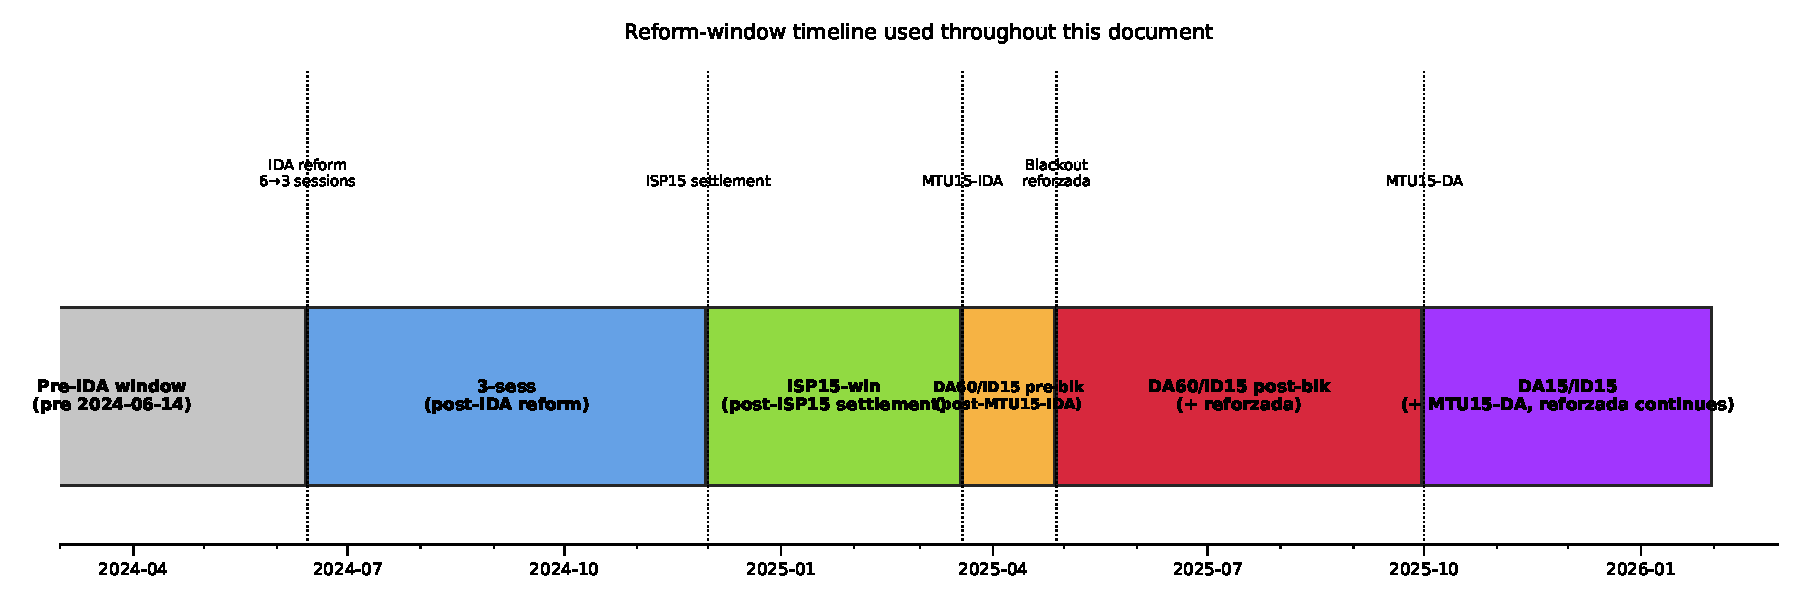
\includegraphics[width=0.95\textwidth]{../../figures/thesis/timeline_reform_windows.pdf}
\caption{\textbf{Reform-window timeline.} Six named windows partition the 2022-2026 sample at the five reform dates. \emph{Pre-IDA}: baseline 6-session IDA, hourly. \emph{3-sess}: post-IDA-reform 3-session IDA, hourly. \emph{ISP15-win}: REE settlement 15-min, OMIE grid still 60-min. \emph{DA60/ID15 pre-blk}: 40-day pre-blackout window with quarter-hourly intraday. \emph{DA60/ID15 post-blk}: post-blackout reforzada, quarter-hourly intraday. \emph{DA15/ID15}: full 15-min grid post-2025-10-01.}
\label{fig:bid_internal:timeline}
\end{figure}

\subsection{In-band region and bid-shape outcomes}\label{sec:data:bandwidth}

\emph{Takeaway.} The bandwidth $\delta = p_{90}-p_{50}$ of the contemporary MCP distribution isolates the \emph{competing tier} of each ladder --- tranches close enough to clearing to be in real contention. Per in-band curve we compute five jointly informative bid-shape statistics: MW-weighted price dispersion $\sigma_p$, intercept $\hat\alpha$ (level), linear slope $\hat\beta$, curvature $\hat\gamma$ (convex $>0$ / concave $<0$), and bid-stack concentration $\text{HHI}_p$ (MW-weighted Herfindahl of in-band tranches). $\sigma_p$ is reported alongside the $(\hat\alpha, \hat\beta, \hat\gamma)$ polynomial fit because it is well-defined on every curve --- including single- and few-tranche curves where the OLS slope is noisy --- and so serves as the robust price-side anchor of the bid-shape DiD.

\paragraph{Bandwidth.} Let $\delta$ be a bandwidth that isolates the tranches in contention --- close enough to the clearing price to compete in the \emph{competing tier} of the offer (CCGT's two-tier structure makes this distinction explicit, Appendix~\ref{app:context}). We anchor $\delta$ to the contemporary contested margin: $\delta = p_{90} - p_{50}$ of the MCP distribution in the analysis window, market by market. The eight bandwidths (one per reform $\times$ \{real, placebo\} $\times$ \{DA, IDA\}) are reported below; wider-$\delta$ robustness in Appendix~\ref{app:robustness}.5.
\begin{center}
\footnotesize
\setlength{\tabcolsep}{8pt}
\begin{tabular}{l c c}
\toprule
\textbf{Window} & $\delta$ in DA (EUR/MWh) & $\delta$ in IDA (EUR/MWh) \\
\midrule
ID15 real             & 50 & 62 \\
ID15 placebo (2024)   & 45 & 46 \\
DA15 real             & 50 & 58 \\
DA15 placebo (2024)   & 45 & 49 \\
\bottomrule
\end{tabular}
\captionof{table}{\textbf{Bandwidths $\delta$ used to define the in-band region.} $\delta$ is set to $p_{90}-p_{50}$ of the MCP distribution in each (window, market). Window-and-market-specific by construction. Bandwidth robustness in \hyperref[sec:5e]{Appendix~\ref*{app:robustness}.5}.}
\end{center}

\begin{figure}[htbp]
\centering
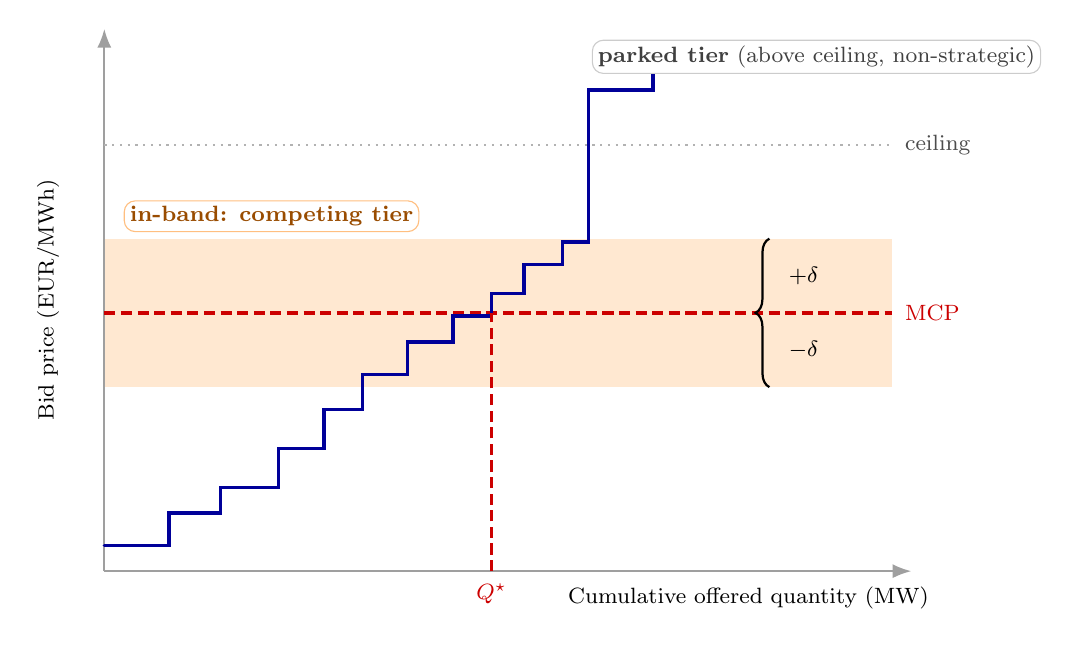
\begin{tikzpicture}[scale=0.82, every node/.style={font=\footnotesize}]
  \def\xmax{12.5}
  \def\ymax{8.4}
  \def\mcp{4}
  \def\h{1.15}
  \def\ceiling{6.6}
  \fill[orange!18] (0, \mcp-\h) rectangle (\xmax-0.3, \mcp+\h);
  \draw[-{Latex[length=2.4mm]}, thick, gray!75] (0,0) -- (\xmax,0)
    node[below left=2pt and -10pt, black] {Cumulative offered quantity (MW)};
  \draw[-{Latex[length=2.4mm]}, thick, gray!75] (0,0) -- (0,\ymax);
  \node[rotate=90, anchor=south, black] at (-0.55, \ymax/2)
    {Bid price (EUR/MWh)};
  \draw[red!80!black, very thick, dash pattern=on 4pt off 2pt]
    (0, \mcp) -- (\xmax-0.3, \mcp);
  \node[red!80!black, anchor=west] at (\xmax-0.25, \mcp) {MCP};
  \draw[gray!60, dotted, thick] (0, \ceiling) -- (\xmax-0.3, \ceiling);
  \node[gray!60!black, anchor=west] at (\xmax-0.25, \ceiling) {ceiling};
  \draw[blue!60!black, very thick, line cap=round]
       (0,    0.4) -- (1.0,  0.4)
    -- (1.0,  0.9) -- (1.8,  0.9)
    -- (1.8,  1.3) -- (2.7,  1.3)
    -- (2.7,  1.9) -- (3.4,  1.9)
    -- (3.4,  2.5) -- (4.0,  2.5)
    -- (4.0,  3.05)-- (4.7,  3.05)
    -- (4.7,  3.55)-- (5.4,  3.55)
    -- (5.4,  3.95)-- (6.0,  3.95)
    -- (6.0,  4.30)-- (6.5,  4.30)
    -- (6.5,  4.75)-- (7.1,  4.75)
    -- (7.1,  5.10)-- (7.5,  5.10)
    -- (7.5,  7.45)-- (8.5,  7.45)
    -- (8.5,  7.75)-- (10.0, 7.75);
  \draw[red!80!black, very thick, dash pattern=on 4pt off 2pt]
    (6.0, 0) -- (6.0, \mcp);
  \node[red!80!black, below] at (6.0, -0.05) {$Q^\star$};
  \draw[decorate, decoration={brace, amplitude=5pt, mirror},
        thick] (\xmax-2.2, \mcp+\h) -- (\xmax-2.2, \mcp-\h);
  \node[anchor=west] at (\xmax-2.05, \mcp+\h/2) {$+\delta$};
  \node[anchor=west] at (\xmax-2.05, \mcp-\h/2) {$-\delta$};
  \node[orange!60!black, anchor=south west, fill=white, rounded corners,
        inner sep=2pt, draw=orange!50, line width=0.4pt]
    at (0.3, \mcp+\h+0.10) {\textbf{in-band: competing tier}};
  \node[gray!50!black, anchor=south west, fill=white, rounded corners,
        inner sep=2pt, draw=gray!40, line width=0.4pt]
    at (7.55, \ceiling+1.1) {\textbf{parked tier} (above ceiling, non-strategic)};
\end{tikzpicture}
\caption{\textbf{Bandwidth $\delta$ and the in-band region.} The blue step function is the sorted sell-bid ladder for one quarter. Only tranches falling within $\pm\delta$ of the clearing price (orange band) enter the bid-shape outcomes; the parked tier above the clearing-price ceiling is excluded (Appendix~\ref{app:context}).}
\label{fig:in-band-bandwidth}
\end{figure}

\begin{figure}[h]
\centering
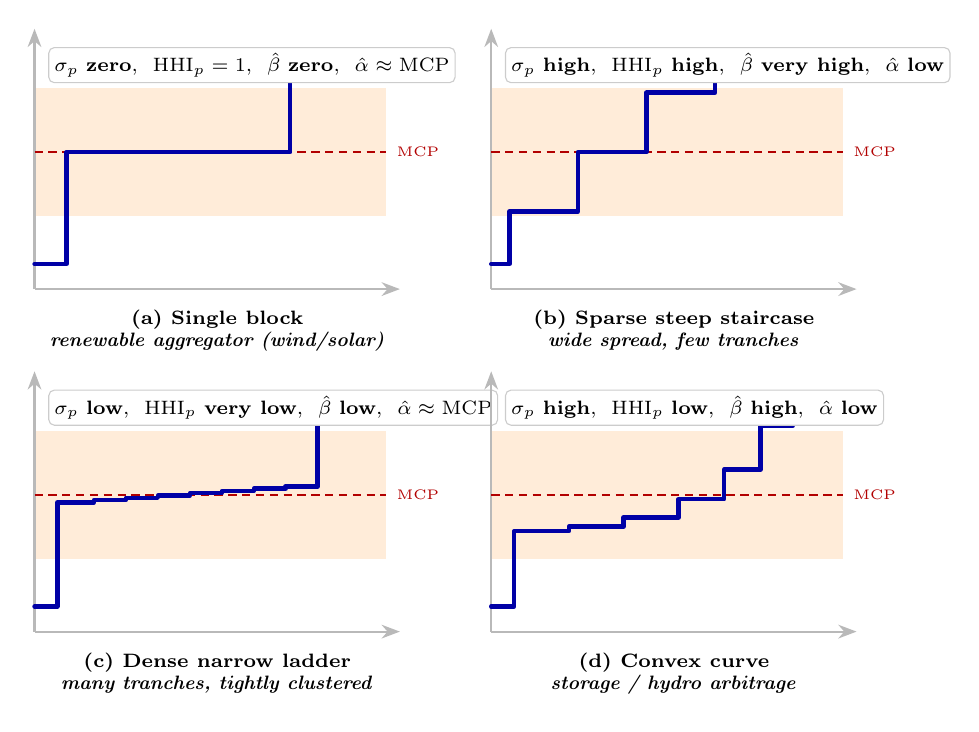
\begin{tikzpicture}[scale=0.58, every node/.style={font=\scriptsize}]
  \def\W{8}
  \def\H{5.4}
  \def\PMCP{3}
  \def\DELTA{1.4}
  \tikzset{
    axis/.style={draw=gray!55, thick, ->, >=Stealth},
    mcp/.style={red!70!black, thick, dash pattern=on 3pt off 2pt},
    band/.style={fill=orange!15},
    ladder/.style={blue!65!black, ultra thick, line cap=round, line join=round},
    plabel/.style={font=\scriptsize\bfseries, anchor=north, align=center},
    outcomes/.style={font=\scriptsize, anchor=north west, fill=white, rounded corners=2pt, inner sep=2pt, draw=gray!40},
  }

  %% ===== Panel (a): Single block (renewable aggregator) =====
  \begin{scope}[xshift=0cm, yshift=0cm]
    \fill[band] (0, \PMCP-\DELTA) rectangle (\W-0.3, \PMCP+\DELTA);
    \draw[axis] (0,0) -- (\W,0); \draw[axis] (0,0) -- (0,\H+0.3);
    \draw[mcp] (0,\PMCP) -- (\W-0.3,\PMCP);
    \node[red!70!black, anchor=west, font=\tiny] at (\W-0.28,\PMCP) {MCP};
    % Low pre-band tranche, then single in-band block at MCP, then post-band tail
    \draw[ladder]
      (0,0.55) -- (0.7,0.55) -- (0.7,3.0) -- (5.6,3.0) -- (5.6,4.9) -- (6.6,4.9);
    \node[outcomes] at (0.3, 5.3)
      {$\sigma_p$ \textbf{zero},\ \ $\text{HHI}_p=1$,\ \ $\hat\beta$ \textbf{zero},\ \ $\hat\alpha \approx \text{MCP}$};
    \node[plabel] at (\W/2,-0.25) {\textbf{(a) Single block} \\ \emph{renewable aggregator (wind/solar)}};
  \end{scope}

  %% ===== Panel (b): Sparse steep staircase (CCGT, few wide steps) =====
  \begin{scope}[xshift=10cm, yshift=0cm]
    \fill[band] (0, \PMCP-\DELTA) rectangle (\W-0.3, \PMCP+\DELTA);
    \draw[axis] (0,0) -- (\W,0); \draw[axis] (0,0) -- (0,\H+0.3);
    \draw[mcp] (0,\PMCP) -- (\W-0.3,\PMCP);
    \node[red!70!black, anchor=west, font=\tiny] at (\W-0.28,\PMCP) {MCP};
    % Pre-band low tranche, then 3 in-band steeply-spaced tranches, then post-band tail
    \draw[ladder]
      (0,0.55) -- (0.4,0.55) -- (0.4,1.7) -- (1.9,1.7) -- (1.9,3.0) -- (3.4,3.0)
      -- (3.4,4.3) -- (4.9,4.3) -- (4.9,5.2) -- (6.0,5.2);
    \node[outcomes] at (0.3, 5.3)
      {$\sigma_p$ \textbf{high},\ \ $\text{HHI}_p$ \textbf{high},\ \ $\hat\beta$ \textbf{very high},\ \ $\hat\alpha$ \textbf{low}};
    \node[plabel] at (\W/2,-0.25) {\textbf{(b) Sparse steep staircase} \\ \emph{wide spread, few tranches}};
  \end{scope}

  %% ===== Panel (c): Dense narrow ladder (many small tranches near MCP) =====
  \begin{scope}[xshift=0cm, yshift=-7.5cm]
    \fill[band] (0, \PMCP-\DELTA) rectangle (\W-0.3, \PMCP+\DELTA);
    \draw[axis] (0,0) -- (\W,0); \draw[axis] (0,0) -- (0,\H+0.3);
    \draw[mcp] (0,\PMCP) -- (\W-0.3,\PMCP);
    \node[red!70!black, anchor=west, font=\tiny] at (\W-0.28,\PMCP) {MCP};
    % Pre-band low tranche, then 8 small in-band steps clustered near MCP, then post-band
    \draw[ladder]
      (0,0.55) -- (0.5,0.55) -- (0.5,2.83) -- (1.3,2.83) -- (1.3,2.88) -- (2.0,2.88)
      -- (2.0,2.93) -- (2.7,2.93) -- (2.7,2.98) -- (3.4,2.98)
      -- (3.4,3.03) -- (4.1,3.03) -- (4.1,3.08) -- (4.8,3.08)
      -- (4.8,3.13) -- (5.5,3.13) -- (5.5,3.18) -- (6.2,3.18)
      -- (6.2,4.9)  -- (6.8,4.9);
    \node[outcomes] at (0.3, 5.3)
      {$\sigma_p$ \textbf{low},\ \ $\text{HHI}_p$ \textbf{very low},\ \ $\hat\beta$ \textbf{low},\ \ $\hat\alpha \approx \text{MCP}$};
    \node[plabel] at (\W/2,-0.25) {\textbf{(c) Dense narrow ladder} \\ \emph{many tranches, tightly clustered}};
  \end{scope}

  %% ===== Panel (d): Convex curve (storage / hydro arbitrage) =====
  \begin{scope}[xshift=10cm, yshift=-7.5cm]
    \fill[band] (0, \PMCP-\DELTA) rectangle (\W-0.3, \PMCP+\DELTA);
    \draw[axis] (0,0) -- (\W,0); \draw[axis] (0,0) -- (0,\H+0.3);
    \draw[mcp] (0,\PMCP) -- (\W-0.3,\PMCP);
    \node[red!70!black, anchor=west, font=\tiny] at (\W-0.28,\PMCP) {MCP};
    % Pre-band low tranche, then convex in-band climb
    \draw[ladder]
      (0,0.55) -- (0.5,0.55) -- (0.5,2.20) -- (1.7,2.20) -- (1.7,2.30) -- (2.9,2.30)
      -- (2.9,2.50) -- (4.1,2.50) -- (4.1,2.90) -- (5.1,2.90)
      -- (5.1,3.55) -- (5.9,3.55) -- (5.9,4.50) -- (6.6,4.50);
    \node[outcomes] at (0.3, 5.3)
      {$\sigma_p$ \textbf{high},\ \ $\text{HHI}_p$ \textbf{low},\ \ $\hat\beta$ \textbf{high},\ \ $\hat\alpha$ \textbf{low}};
    \node[plabel] at (\W/2,-0.25) {\textbf{(d) Convex curve} \\ \emph{storage / hydro arbitrage}};
  \end{scope}
\end{tikzpicture}
\caption{\textbf{Four stylized in-band bid shapes spanning the $(\sigma_p, \text{HHI}_p, \hat\beta, \hat\alpha)$ space.} Each panel shows one bid ladder against a common MCP (red dotted) and bandwidth $\delta$ (orange band), with the implied outcome values noted in the corner.}
\label{fig:bid-shape-stylized}
\end{figure}

\paragraph{In-band set.} For each $(u,d,p)$ curve:
\[
\mathcal{B}_{u,d,p} \;=\; \bigl\{k:\;|p_k - \text{MCP}_{d,p}| \le \delta\bigr\}, \qquad
w_k = \frac{\Delta q_k}{\sum_{j\in\mathcal{B}_{u,d,p}} \Delta q_j}, \qquad
\bar p_{u,d,p} = \sum_{k\in\mathcal{B}} w_k\, p_k.
\]
Representative bid curves per technology in critical and flat hours are in Appendix~\ref{app:context}.4 (Figures~\ref{fig:bid-curves-by-tech}--\ref{fig:bid-curves-by-tech-flat}); they illustrate the dispatchable-ladder vs renewable-block contrast.

\paragraph{Four bid-shape outcomes.} Per curve, the in-band tranches deliver four non-redundant summaries.

\emph{Level, slope, curvature (two-stage unweighted OLS on in-band step endpoints).} Let $Q_k = \sum_{j\le k}\Delta q_j$ be the cumulative in-band MW after the $k$th tranche. We fit two separate OLS regressions on the in-band tranches, each with equal weight per tranche (no MW weighting). First, a \emph{linear} fit recovers the level and the average slope:
\[
p_k \;=\; \hat\alpha_{u,d,p} + \hat\beta_{u,d,p}\,Q_k + e_k.
\]
Second, a \emph{quadratic} fit recovers the curvature term (we keep only the quadratic coefficient from this regression; the implied linear coefficients of the quadratic regression differ from $\hat\alpha, \hat\beta$ and are not used):
\[
p_k \;=\; \tilde\alpha_{u,d,p} + \tilde\beta_{u,d,p}\,Q_k + \hat\gamma_{u,d,p}\,Q_k^2 + \tilde e_k.
\]
The two-stage construction keeps the interpretation of each coefficient clean. $\hat\alpha$ is the geometric level of the ladder (predicted price at $Q=0$ under the linear projection of the in-band steps). $\hat\beta$ is the average linear slope (EUR/MWh per MW) and is the direct empirical counterpart of the model's per-product residual-demand slope $b_{mt}$ (\S\ref{sec:theory:setup}). $\hat\gamma$ is the curvature: $\hat\gamma > 0$ means the curve bends \emph{convex} (slope steepens with $Q$, the bidder packs cheap MW at the bottom and asks higher prices for the marginal MW); $\hat\gamma < 0$ means \emph{concave} (steep climb early then a flatter tail); $\hat\gamma$ is the part of curvature orthogonal to the linear trend (by Frisch--Waugh, the quadratic-regression coefficient on $Q_k^2$ equals the slope of $p_k$-residuals on $Q_k^2$-residuals after both are linearly netted of $Q_k$). With $K=2$ in-band tranches only $\hat\alpha, \hat\beta$ are identified; $\hat\gamma$ requires $K\ge 3$.

\emph{Bid-stack concentration.}
\[
\text{HHI}_{p,\,u,d,p} \;=\; \sum_{k\in\mathcal{B}} w_k^2, \qquad w_k = \frac{\Delta q_k}{\sum_{j\in\mathcal{B}}\Delta q_j}.
\]
MW-weighted Herfindahl of in-band tranches, bounded in $[1/|\mathcal{B}|,\,1]$. $\text{HHI}_p = 1$ means a single in-band block (MW fully concentrated); $\text{HHI}_p = 1/K$ means $K$ equal-sized tranches (maximally dispersed). $\text{HHI}_p$ captures the concentration of the bidder's in-band MW; $(\hat\alpha, \hat\beta, \hat\gamma)$ capture the smooth shape that fits those tranches. The equivalent effective-tranche-count framing $N_{\text{eff}} = 1/\text{HHI}_p$ is used in some granularity papers; we use HHI to keep the IO-native concentration reading.

\emph{What each outcome captures.} The five outcomes are jointly informative and non-redundant: $\sigma_p$ is the MW-weighted price dispersion within the band, $\hat\alpha$ is level, $\hat\beta$ is linear slope, $\hat\gamma$ is curvature (convex/concave), $\text{HHI}_p$ is bid-stack concentration. Reading them together disentangles how much price spread the in-band MW carries, where the curve sits, how steep it is, whether it bends, and how the MW is split across tranches. None depends on price-level seasonality since all are computed relative to the contemporaneous MCP via the bandwidth $\delta$. Figure~\ref{fig:bid-shape-stylized} illustrates the outcomes on stylised ladders.

\emph{Price-side dispersion.}
\[
\sigma_{p,\,u,d,p} \;=\; \Big[\sum_{k\in\mathcal{B}} w_k \,(p_k - \bar p_{u,d,p})^2\Big]^{1/2},
\]
with $w_k$ and $\bar p_{u,d,p}$ as defined in the in-band set above. Each tranche is weighted by its MW share $w_k$, so $\bar p_{u,d,p}$ is the average price the firm receives per representative in-band MW (not per tranche) and $\sigma_p$ is the typical price spread per representative MW. The MW-weighting is the economically correct one: a 100~MW tranche at $\bar p + 5$ contributes $100\times$ the profit-uncertainty of a 1~MW tranche at $\bar p + 5$, so big tranches drive $\sigma_p$ and decoy micro-tranches at distant prices barely move it. Consequences: a single in-band tranche contributes $\sigma_p=0$; a symmetric large-large split at $\bar p \pm \Delta$ gives $\sigma_p=\Delta$; and $\sigma_p$ is bounded by the half-bandwidth $\delta$ for any in-band curve. For near-linear curves $\sigma_p \approx |\hat\beta|\,\sigma_Q$, so it carries the same content as the slope outcome up to estimator noise, but $\sigma_p$ requires only $p$-side variation and is well-defined on every curve (including single-tranche and few-tranche curves where the OLS slope is noisy). It is therefore the robust price-side anchor of the bid-shape decomposition rather than a fallback. The parallel-trends figure in \S\ref{sec:5b} leads with $\sigma_p$ (Figure~\ref{fig:parallel-trends-sigma-p}) and reports the $(\hat\alpha, \hat\beta, \hat\gamma, \text{HHI}_p)$ structural decomposition alongside (Figure~\ref{fig:parallel-trends-abgN}); the DiD table in \S\ref{sec:results:6-2} reports all five outcomes side by side.

\subsection{Aggregate outcomes}\label{sec:data:aggregate}

\emph{Takeaway.} Five system-level outcomes built off the bid-stack and the cleared prices: in-band offered energy per (tech, market, day, hour-class); the day-ahead/intraday wedge $\Delta_{d,h}$ and its within-day SD $\Delta^{\text{SD}}_d$; the intraday-auction in-band sell-share by tech; system ajuste cost (per day, EUR\,M); and five post-MTU15-only within-hour dispersion outcomes $D^{\bullet}_{d,h}$ that summarise across-quarter shifts in price level, volume, system MCP, ladder spread, and tranche count. The wedge SD $\Delta^{\text{SD}}_d$ and the IDA in-band sell-share are the load-bearing system-level outcomes for Spec~A.

\paragraph{In-band offered energy} (per (tech, market, day, hour-class)). Per-curve in-band MW: $m_{u,d,p} = \sum_{k\in\mathcal{B}_{u,d,p}} \Delta q_k$. Aggregated to tech $t$, market $m$, hour-class $\mathcal{X}$, and converted to energy with $\tau_p$ the period length in hours ($\tau_p = 1$ pre-MTU15, $\tau_p = 1/4$ post-MTU15):
\[
E^{\text{band}}_{t,m,d,\mathcal{X}} \;=\; \frac{1}{|\mathcal{X}|}\sum_{h\in\mathcal{X}}\,\sum_{p\in h}\,\sum_{u\in t} m_{u,d,p}\cdot\tau_p \qquad \text{(MWh per class-hour)}.
\]
The $\tau_p$ factor makes the post-MTU15 quarter-sum invariant to the period count; the $1/|\mathcal{X}|$ normalisation makes levels comparable across hour-classes of different sizes.

\paragraph{Cross-market wedge} (per clock-hour). Let $\text{MCP}^{\text{DA}}_{d,h}$ and $\text{MCP}^{\text{IDA}}_{d,h}$ be the within-market means of the OMIE clearing prices over whatever sub-hour structure each market has on date $d$ (DA collapses four quarters post-DA15; IDA collapses three sessions and, post-ID15, four quarters):
\[
\Delta_{d,h} \;=\; \text{MCP}^{\text{DA}}_{d,h} - \text{MCP}^{\text{IDA}}_{d,h}, \qquad
\Delta^{\text{SD}}_d \;=\; \mathrm{sd}_h(\Delta_{d,h}).
\]
$\Delta_{d,h}$ is the DA$-$IDA gap (EUR/MWh) at clock-hour $h$; $\Delta^{\text{SD}}_d$ summarises how that gap varies across the 24 clock-hours of day $d$. The clock-hour collapse makes $\Delta_{d,h}$ directly comparable across regimes (it does not widen mechanically when IDA gains a quarter dimension).

\paragraph{IDA in-band sell-share} (per (tech, day)). Restricted to in-band tranches:
\[
\text{SS}_{t,d} \;=\; \frac{\sum_{q,k\in\mathcal{B}} q^{\text{sell}}_{t,d,q,k}}{\sum_{q,k\in\mathcal{B}}\bigl(q^{\text{sell}}_{t,d,q,k} + q^{\text{buy}}_{t,d,q,k}\bigr)}.
\]
Captures the position of production units between sell-heavy (rent-capture) and buy-heavy (rebalancing) participation in the intraday auction.

\paragraph{System ajuste cost} (per day, EUR/M). REE's adjustment-cost components from ESIOS: up-direction (TR-up, aFRR-up, mFRR-up, Fase~I) and down-direction (Fase~II, RR-dn), stacked positive in Figure~\ref{fig:efficiency_gains}.

\paragraph{Within-hour dispersion outcomes} (post-MTU15 only). For each (unit, date, clock-hour) with four quarters $q=1,\ldots,4$:
\[
D^{\bar p}_{d,h} = \mathrm{sd}_q(\bar p_q), \quad
D^{m}_{d,h} = \mathrm{sd}_q(m_q)/\bar m, \quad
D^{\text{MCP}}_{d,h} = \mathrm{sd}_q(\text{MCP}_q), \quad
D^{\sigma_p}_{d,h} = \mathrm{sd}_q(\sigma_{p,q}), \quad
D^{\text{HHI}}_{d,h} = \mathrm{sd}_q(\text{HHI}_{p,q}).
\]
The five $D^\bullet_{d,h}$ outcomes capture across-quarter shifts in price level, volume, system MCP, ladder spread and tranche count. All are mechanically zero under MTU60 (one quarter per clock-hour), so any positive value post-MTU15 is a direct trace of within-hour discrimination. These are used in \S\ref{sec:data:partition} to characterise where within-hour discrimination concentrates.

\subsection{Critical / flat hour-class partition}\label{sec:data:partition}

\emph{Takeaway.} Granular pricing has economic content only where within-hour residual demand actually varies. Measured by 15-minute residual-demand SD, clock-hours partition into critical (morning ramp 5--8h, evening ramp 16--22h; SD 522--1303 MW), flat (overnight 1--3h; SD 336--357 MW), and midday (11--14h; SD 468--502 MW, kept for falsification only). Spec~C uses critical-vs-flat as the within-day identification contrast.

\paragraph{Intuition.} Granular pricing only has economic content where within-hour residual demand\footnote{Spanish-market convention calls this the \emph{hueco t\'ermico} (thermal gap) --- the load that thermal and other dispatchable generation must cover after subtracting wind and solar.} actually varies; if a clock-hour is internally flat, the four quarters look the same and there is nothing to discriminate on. We measure within-hour variation by $\sigma_{\text{within}}(h,d) = \mathrm{sd}_q[\text{load}-\text{wind}-\text{solar}]_{q,h,d}$ on 15-min ENTSO-E data (A65 load; A75 PSR codes B16, B18, B19 for wind+solar) and partition clock-hours by median $\sigma_{\text{within}}$ post-2024-06-14:
\begin{itemize}\setlength{\itemsep}{1pt}
\item \textbf{Critical} $\mathcal{C}=\mathcal{C}_M\cup\mathcal{C}_E$ with $\mathcal{C}_M=\{5,\dots,8\}$ (morning ramp) and $\mathcal{C}_E=\{16,\dots,22\}$ (evening ramp); $\sigma_{\text{within}}\in[522,1303]$ MW.
\item \textbf{Flat} $\mathcal{F}=\{1,2,3\}$: overnight; $\sigma_{\text{within}}\in[336,357]$ MW.
\item \textbf{Midday} $\mathcal{M}=\{11,\dots,14\}$ (solar-marginal, $\sigma_{\text{within}}\in[468,502]$ MW): excluded from main specs; kept for falsification (Appendix~\ref{app:robustness}.2).
\end{itemize}

\paragraph{Descriptive critical $-$ flat differential.} Let $D^\bullet_{d,h}$ stand for any one of the five within-hour dispersion outcomes of \S\ref{sec:data:aggregate} on date $d$, clock-hour $h$. Fit per outcome on the post-MTU15 sample, $h\in\mathcal{C}\cup\mathcal{F}$:
\[
D^\bullet_{d,h} \;=\; \eta_d \;+\; \theta\,\mathbf{1}\{h\in\mathcal{C}\} \;+\; \varepsilon_{d,h}
\]
with date fixed effects $\eta_d$ (distinct from the bandwidth $\delta$). $\theta$ is the critical$-$flat dispersion gap; a descriptive contrast, not a causal estimate.

\begin{center}
\footnotesize
\setlength{\tabcolsep}{6pt}
\begin{tabular}{l l c c c}
\toprule
\textbf{Outcome} & \textbf{Subsample} & \textbf{ID15} & \textbf{DA15} & \textbf{crit/flat ratio (IDA, DA)} \\
\midrule
$D^{\bar p}$ (EUR/MWh)              & per unit (pooled) & $\mathbf{0.39}^{***}$ (0.05)    & $\mathbf{1.35}^{***}$ (0.11)   & $4.1\times,\ \mathbf{7.4\times}$ \\
$D^{m}$ (CV)                        & per unit (pooled) & $\mathbf{0.024}^{***}$ (0.003)  & $\mathbf{0.033}^{***}$ (0.002) & $4.3\times,\ 4.9\times$ \\
$D^{\text{MCP}}$ (EUR/MWh)          & system            & $\mathbf{4.55}^{***}$ (0.40)    & $\mathbf{3.97}^{***}$ (0.37)   & $2.8\times,\ 2.6\times$ \\
\addlinespace
$D^{\sigma_p}$ (EUR/MWh)            & CCGT       & $-0.19$ (0.36)         & $\mathbf{0.61}^{***}$ (0.12)    & $0.8\times,\ \mathbf{6.5\times}$ \\
                                    & Hydro      & $\mathbf{0.48}^{***}$ (0.08)    & $\mathbf{1.32}^{***}$ (0.17)    & $2.2\times,\ 3.3\times$ \\
                                    & Hydro pump & $\mathbf{0.14}^{***}$ (0.03)    & $\mathbf{0.70}^{***}$ (0.17)    & $3.3\times,\ 10.9\times$ \\
                                    & Wind       & $0.00$ (0.01)          & $0.03^{**}$ (0.01)              & $0.9\times,\ 1.9\times$ \\
\addlinespace
$D^{1/\text{HHI}}$                  & CCGT       & $0.17$ (0.16)          & $\mathbf{0.17}^{***}$ (0.02)    & $1.1\times,\ \mathbf{14.3\times}$ \\
                                    & Hydro      & $\mathbf{0.05}^{***}$ (0.01)    & $\mathbf{0.19}^{***}$ (0.03)    & $2.0\times,\ 2.8\times$ \\
                                    & Hydro pump & $\mathbf{0.03}^{***}$ (0.01)    & $\mathbf{0.13}^{***}$ (0.03)    & $2.6\times,\ 4.3\times$ \\
                                    & Wind       & $0.00$ (0.00)          & $0.01$ (0.00)                   & $1.0\times,\ 1.3\times$ \\
\bottomrule
\end{tabular}
\captionof{table}{\textbf{Post-MTU15 critical$-$flat within-hour dispersion gap $\theta$, by outcome.} Post-only cross-sectional gap. Windows: ID15 post 2025-03-19 to 2025-04-27; DA15 post 2025-10-01 to 2025-12-31. SE clustered by date; $^{*}p<0.10$, $^{**}p<0.05$, $^{***}p<0.01$ (applies to all subsequent tables). Bid-level rows ($D^{\bar p}$, $D^{m}$, $D^{\text{MCP}}$) are bandwidth-free; the per-tech $D^{\sigma_p}$ and $D^{1/\text{HHI}}$ rows use the window-specific $p_{90}$ bandwidth (\S\ref{sec:data:bandwidth}): ID15 column $\delta{=}62$ (post-ID15 IDA); DA15 column $\delta{=}50$ (post-DA15 DA). $D^{1/\text{HHI}}$ uses the effective-tranche-count framing ($N_{\text{eff}} = 1/\text{HHI}_p$) because the within-hour SD of HHI is mechanically tiny on a $[0,1]$ scale; the inverse-HHI quantity carries the same content on a more readable scale.}
\end{center}

% =====================================================================
\section{Empirical strategy: three specifications for three economic objects}\label{sec:empirical}
% =====================================================================

Indices follow \S\ref{sec:data:outcomes}. The Spec~C treatment indicator is $\mathbf{1}\{d\ge T_r\}\cdot\mathbf{1}\{h(p)\in\mathcal{C}\}$ with the sample restricted to $h(p)\in\mathcal{C}\cup\mathcal{F}$.

\subsection{Spec A: Bayesian Structural Time Series for prices, cleared energy, and wedge SD}\label{sec:empirical:specA}

\emph{Takeaway.} Spec~A is the Bayesian state-space counterfactual: train on a long pre-window with year-by-year wind and solar interactions, extrapolate forward to the post-window, read the treatment effect as the gap between observed and counterfactual. The year-by-year renewable interactions are the load-bearing element --- Spanish wind+solar capacity grew $\sim$$6\times$ over 2018--2025, so a flat coefficient mis-fits the cross-year merit-order shift. A 2024 same-calendar placebo with a fake cutover guards against recurring seasonal artefacts.

\emph{Model.} The daily response decomposes additively into trend, weekly cycle, exogenous covariates, and noise:
\[
y_t \;=\; \underbrace{\mu_t}_{\text{trend}} \;+\; \underbrace{\gamma_t}_{\text{weekly cycle}} \;+\; \underbrace{X_t'\beta}_{\text{exogenous covariates}} \;+\; \underbrace{\varepsilon_t}_{\text{noise}}.
\]
$\mu_t$ is a random walk with stochastic slope, $\gamma_t$ a 7-day cycle, and $X_t$ a covariate vector consisting of contemporaneous wind GWh, solar GWh, gas price (EUR/MWh), and the interactions $\text{wind}_t \times \mathbf{1}\{\text{year}(t)=y\}$ and $\text{solar}_t \times \mathbf{1}\{\text{year}(t)=y\}$ for each calendar year $y$ in the pre-window. A spike-and-slab prior on $\beta$ shrinks unused regressors. Demand is excluded to avoid simultaneity. Fitted via the \texttt{CausalImpact} R package \citep{brodersen_2015}; the architecture is the EPEX 15-min reform spec of \citet{markle_huss_2017}.

\emph{Outcomes $y_t$.} DA or IDA daily-average clearing prices, per-tech daily cleared GWh, within-day wedge SD $\Delta^{\text{SD}}_d$ overall and per hour-class $\Delta^{\text{SD},\mathcal{X}}_d = \mathrm{sd}_{h\in\mathcal{X}}(\Delta_{d,h})$ for $\mathcal{X}\in\{\mathcal{C}_M, \mathcal{C}_E, \mathcal{M},\mathcal{F}\}$, and per-tech IDA in-band sell-share $\text{SS}_{t,d} = \sum q^{\text{sell, in-band}}_{t,d} / \sum (q^{\text{sell, in-band}}_{t,d}+q^{\text{buy, in-band}}_{t,d})$ (\S\ref{sec:results:6-6b}).

\emph{Estimand.} Conditional on $X_t$, the post-cutover counterfactual equals the pre-trained extrapolation $\hat y_t(0)$. The average treatment effect on the post-window is
\[
\bar\tau \;=\; \tfrac{1}{|\text{post}|}\textstyle\sum_{t\ge T_r}\bigl(y_t - \hat y_t(0)\bigr),
\]
reported together with its 95\% credible interval from the MCMC posterior produced by the \texttt{CausalImpact} R package.

\emph{Windows.} Pre-windows are long: 2022-01-01 onwards through the day before each reform cutover. The long pre-window is what makes the year-by-year renewable interaction identified (each calendar year contributes its own renewable response). Post-windows are short: $40$ days at each cutover. For ID15 the $40$-day post-window stops at the April 2025 blackout; for DA15 the pre-window straddles the blackout so the post-window does not need a separate reforzada-constant truncation.

\emph{Placebo cross-check.} The same BSTS is re-run on a same-calendar window one year before each reform with a fake cutover. The real-window 95\% credible interval must exclude zero AND the placebo must be either null or opposite-signed for a finding to be retained as a reform-attributable effect; placebos that move in the same direction as the real estimate flag a recurring calendar shift the seasonality model has not absorbed.

\emph{MCMC and prior settings.}\phantomsection\label{sec:empirical:drift} $\texttt{niter}=2{,}000$ MCMC iterations after burn-in (a $5\times$ increase changes point estimates and 95\% intervals by $<2\%$ across all reported cells, Appendix~\ref{app:robustness}.1). $\texttt{prior.level.sd}=0.005$ as a fraction of the response SD; the result is insensitive to this choice over $[0.005, 0.01]$ but distorts under an aggressive $0.001$ (Appendix~\ref{app:robustness}.1).

\subsection{Spec B: per-hour-class BSTS on in-band offered energy}\label{sec:empirical:specB}

\emph{Takeaway.} Spec~B is Spec~A applied per (tech, market, hour-class) cell with the in-band offered-energy outcome. It lets the data reveal any critical-hour concentration as heterogeneity across hour classes rather than imposing the critical/flat differential as the identifying restriction. Under the year-interaction control no Spec~B cell survives as a retained finding; the bid-shape DiD of Spec~C provides the cleaner within-day identification on the same channel.

\subsection{Spec C: per-curve DiD for bid shape}\label{sec:empirical:specC}

\emph{Takeaway.} Spec~C identifies WITHIN-DAY changes in the bid curve: per (unit, date, period) we summarise the in-band ladder with five jointly informative statistics (price dispersion $\sigma_p$, intercept $\alpha$, slope $\beta$, curvature $\gamma$, bid-stack concentration $\text{HHI}_p$) and run a DiD that uses flat hours as the within-day control for critical hours. The flat-hour partition is the identifying restriction; no time-series extrapolation is needed.

For per-tech bid-shape outcomes $Y\in\{\sigma_p, \hat\alpha, \hat\beta, \hat\gamma, \text{HHI}_p\}$ (see \S\ref{sec:data:bandwidth}; $\sigma_p$ is the robust price-side anchor, well-defined on every curve including those where the OLS polynomial slope is noisy) we use the DiD:
\[
Y_{u,d,p[,s]} = \alpha_u + \beta\,\mathbf{1}\{d\ge T_r\} + \xi\,\mathbf{1}\{h\in\mathcal{C}\} + \theta\,D_{d,h} + \varepsilon, \qquad \text{SEs clustered by date.}
\]
The bid-shape coordinates $(\hat\alpha_{u,d,p}, \hat\beta_{u,d,p}, \hat\gamma_{u,d,p})$ are computed per curve in the two-stage construction of \S\ref{sec:data:bandwidth}: $\hat\alpha$ and $\hat\beta$ from a linear OLS of price on cumulative in-band MW, $\hat\gamma$ from a separate quadratic OLS on the same sample. $\text{HHI}_p = \sum_{k\in\mathcal{B}} w_k^2$ is the MW-weighted Herfindahl of in-band tranches (bounded $[1/|\mathcal{B}|,1]$).

\textbf{The granularity reform's bid-shape effect is structurally a critical-hours effect.} Differentiated bidding only pays off where the residual demand curve is steep enough to reward it: in critical hours that condition holds, so 4 quarter-prices instead of 1 unlock real price discrimination; in flat hours the curve is shallow and the extra granularity is mostly wasted optionality. The (critical $-$ flat) differential $\theta$ therefore IS the granularity-enabled discrimination, not a residual we are netting out. Flat hours act as a low-exposure within-day control. Each reform is studied separately, so the design is a standard 2$\times$2 DiD without staggered-treatment complications \citep[ch.~3]{de_chaisemartin_2026}.

% =====================================================================
\section{Results}\label{sec:results}
% =====================================================================

\noindent We organise the empirical findings around the three first-order questions a reader would ask about the reform:

\smallskip
\begin{enumerate}\setlength{\itemsep}{2pt}
  \item \textbf{Did prices drop at each reform? Were there cross-market effects?} (\S\ref{sec:results:Q1}). \textbf{Yes at ID15, null at DA15.} The pricing-chain INPUT (per-firm $b_{mt}$ thickening on every dominant firm at both reforms) is robust. The OUTPUT (BSTS clearing-price effect on the granular leg) is $-34$ EUR/MWh at ID15 IDA --- robust across a $-23$ to $-41$ range even under a \emph{calibrated-solar counterfactual} that explicitly pre-subtracts solar's strong 2024 marginal effect ($-0.46$) from observed prices before fitting BSTS (Appendix~\ref{app:solar-year-coefs}). The DA15 DA effect is null across every calibration we tried. The cross-market level effect is also null; the cross-market response shows up on the bid \emph{shape} (DA anticipates the IDA reform), not on the price level.
  \item \textbf{Did aggregate imbalance volumes drop? Are renewables better off?} (\S\ref{sec:results:Q2}). Aggregate imbalance volume is statistically unchanged at both reforms. The regulatory BS3 imbalance penalty per absolute MWh of deviation drops by roughly a third at each reform. On the system-cost line, real-time channels fall while Fase~I rises; we treat the bulk of the real-time fall as a procurement-timing displacement inside the post-blackout regime, not a granularity efficiency gain. Renewable welfare effects are mixed: wind sells more actively in IDA; nuclear's auction-plus-bilateral output drops sharply in the 40 days post-March.
  \item \textbf{Did wedges close, arbitrage improve, and quantity shift to the granular market?} (\S\ref{sec:results:Q3}). The DA$-$IDA wedge \emph{mean} stays positive in every regime (granularity does not collapse it); the within-day wedge \emph{SD} jumps at the spot reform and does not revert at the forward reform --- the empirical fingerprint of bounded per-product arbitrage. Production-unit arbitrageurs are empirically active on the IDA bid stack; IDA sell-share rises sharply for nuclear and wind; CCGT restructures its DA bid stack in critical hours. Quantity shift to the granular market is partial: present on the participation margin (nuclear, wind) and on the bid stack (CCGT bid-shape restructuring), absent on CCGT's DA/IDA portfolio mix.
\end{enumerate}

\smallskip
\noindent On identification: Spec~C does the bid-shape DiD within day; Spec~A does the BSTS counterfactual on level outcomes with year-by-year renewable interactions. Several level shifts the model predicts have the right sign but credible intervals that bracket zero under the strictest year-interaction spec; we report them as supportive rather than headline. \S\ref{sec:results:synthesis} closes by reading the four answers as one story.

\subsection{Q1 --- Prices in each reform and cross-market effects}\label{sec:results:6-3}\phantomsection\label{sec:results:Q1}
\phantomsection\label{sec:results:6-2}
\phantomsection\label{sec:results:6-4}
\phantomsection\label{tab:specB-id15}
\phantomsection\label{tab:specB-da15}
\phantomsection\label{fig:bsts-id15}
\phantomsection\label{fig:bsts-da15}

\emph{Takeaway.} The model's pricing chain has two links. The first is the model's input: a residual-demand slope $b_{mt}$ that each firm sees. A larger $b_{mt}$ means thicker competition per product, which by the Cournot first-order condition $\text{markup}=q_m/b_{mt}$ shrinks the firm's markup. The second link is the equilibrium output: a lower clearing price. The data deliver the first link robustly. Per-firm $b_{mt}$ thickens for every one of the four dominant CCGT-owning firms after each reform, the direction survives a long-pre window with year and calendar-month fixed effects (firm-by-firm ratio $+8$\%--$+15$\% under controls, significant in every cell; Appendix~\ref{app:robustness}.10). The second link is also delivered. Under the per-year BSTS spec the clearing-price effect on the granular leg is $-34$ EUR/MWh at ID15 IDA (placebo-net $-12$, $p=0.10$) and null at DA15 DA. We considered the concern that the BSTS post-window prediction under-credits solar's marginal effect (since the ID15 2025 year-dummy is fitted on Jan-Mar 2025 only) and implemented a calibrated-solar counterfactual that pre-subtracts solar's 2024-conditional contribution ($-0.46$ EUR/MWh per GWh) before fitting BSTS, then adds it back in the prediction. The ID15 IDA price drop survives ($-26$ EUR/MWh real, $-63$ after 2024-same-calendar placebo-netting); the DA15 DA effect remains null ($+9$ real, $-13$ net). The full robustness table is in Appendix~\ref{app:solar-year-coefs}. Three other model-predicted level shifts (cleared-MWh scale-up, in-band offered-energy migration, renewable cleared-MW reallocation) have the right sign but their credible intervals bracket zero once the renewable coefficient is allowed to vary across years; we report them as supportive but not headline.

\paragraph{The headline match: input thickens, price falls (magnitude methodology-sensitive).} Table~\ref{tab:cournot-match} pairs the two sides of equation~\eqref{eq:cournot-markup} for the two reform-side legs. The left column shows the model's INPUT --- the per-firm residual-demand slope $b_{mt}$ ratio (post/pre) recovered following \citet{ito_reguant_2016}'s strategy: larger than one in every cell, for every dominant firm. The right column shows the model's OUTPUT --- the BSTS clearing-price effect: $-34$ EUR/MWh at ID15 IDA and null at DA15 DA under the per-year spec, with the ID15 magnitude landing in a $-22$ to $-45$ EUR/MWh range across alternative year-coefficient specifications (Appendix~\ref{app:solar-year-coefs}). The per-firm-slope channel is the cleanly identified primitive; the equilibrium-price channel is robust in sign at ID15 IDA but methodology-sensitive in magnitude, consistent with the price level being co-determined with renewables, gas, and the post-blackout regime in ways the BSTS state-space model has limited power to disentangle. At DA15 DA the price channel is null under every spec we tried.

\begin{center}
\footnotesize
\setlength{\tabcolsep}{6pt}
\renewcommand{\arraystretch}{1.20}
\begin{tabular}{l c c}
\toprule
                       & \textbf{Per-firm residual-demand slope} & \textbf{Equilibrium clearing price} \\
\textbf{Reform-side leg} & \emph{ratio} $b^{\text{post}}_{mt}/b^{\text{pre}}_m$ (4-firm range) & \emph{BSTS effect} (EUR/MWh, placebo-net) \\
\midrule
ID15 IDA (granular spot)   & $1.15$--$1.23$ & $-34$ \quad (placebo $-22$ $\Rightarrow$ net $-12$) \\
DA15 DA  (granular forward) & $1.24$--$1.28$ & $+8$ \quad (placebo $+4$ $\Rightarrow$ net $+4$, null) \\
\bottomrule
\end{tabular}
\captionof{table}{\textbf{Headline match between model primitive and equilibrium price.} Windows: ID15 pre 2024-06-14 to 2025-03-18, post 2025-03-19 to 2025-04-27 (pre-blackout); DA15 pre 2024-06-14 to 2025-09-30, post 2025-10-01 to 2025-12-31. BSTS pre-window starts 2022-01-01 with per-year wind and solar interactions; placebo is the same window with the cutover shifted one year earlier. Left: per-firm residual-demand slope $b_{mt}$ ratio post/pre, range across the four dominant CCGT-owning firms (\hyperref[tab:per-firm-residual-demand]{Appendix Table~\ref*{tab:per-firm-residual-demand}}). Larger ratio $=$ thicker per-firm residual demand $=$ smaller per-firm Cournot markup $q_m/b_{mt}$. Right: BSTS effect on the granular-leg clearing price. The model predicts: $b_{mt}$ thicker $\Rightarrow$ markup down $\Rightarrow$ price down. The per-firm slope thickens robustly at both reforms (left). The BSTS price effect (right) is robustly negative-in-sign at ID15 IDA across a range of year-coefficient specifications ($-22$ to $-45$ EUR/MWh; see the robustness table in Appendix~\ref{app:solar-year-coefs}) and null at DA15 DA under every spec we tried. The ID15 magnitude is methodology-sensitive but does not flip sign.}
\label{tab:cournot-match}
\end{center}

The sign match is unambiguous. The magnitude check is more nuanced. The elasticity channel alone --- a roughly proportional markup compression from the $b_{mt}$ thickening --- predicts a single-digit EUR/MWh price drop at baseline tight-hour markups. The data show a larger drop. The most natural reading is that the elasticity channel does what the model says it does, but it operates alongside the other reform-attributable mechanisms (sell-side participation migration of \S\ref{sec:results:6-6b}, in-band offered-energy migration, rationalised dispatch absorbed at the auction). The model's elasticity channel is one structurally-identified piece of a larger reform-driven movement, not the whole story.

Spec~A applies BSTS to system-level outcomes: clearing prices, per-tech daily cleared GWh, and the within-day wedge SD $\Delta^{\text{SD}}_d$. Table~\ref{tab:bsts-spec-a} reports the Real, Placebo, and placebo-net (Net) posterior means for each outcome and each reform.

\begin{center}
\footnotesize
\setlength{\tabcolsep}{8pt}
\renewcommand{\arraystretch}{1.15}
\begin{tabular}{l c c}
\toprule
\textbf{Outcome} & \textbf{ID15 real} & \textbf{2024 placebo} \\
\midrule
\multicolumn{3}{l}{\emph{Within-hour DA$-$IDA wedge SD (EUR/MWh)}} \\
\hspace{0.3em}Overall        & $\mathbf{1.15}^{**}$  & $-0.96$ \\
\hspace{0.3em}Critical hours & $\mathbf{2.12}^{***}$ & $-0.68$ \\
\addlinespace
\multicolumn{3}{l}{\emph{IDA in-band sell-share (pp)}} \\
\hspace{0.3em}Nuclear        & $\mathbf{33.5}^{***}$ & n/a \\
\hspace{0.3em}Wind           & $\mathbf{23.5}^{***}$ & n/a \\
\bottomrule
\end{tabular}
\captionof{table}{Retained Spec~A findings (long-pre BSTS, pre-window 2022-01-01 onwards with year-by-year renewable interactions). ID15 post-window 2025-03-19 to 2025-04-27 (pre-blackout). 2024 placebo same calendar window with cutover shifted one year earlier (real reform absent). Full table in Appendix~\ref{app:robustness}.1.}
\label{tab:bsts-spec-a}
\end{center}


\subsection{Q2 --- Aggregate imbalance volume and regulatory imbalance penalty (Spec A)}\label{sec:results:Q2}\phantomsection\label{sec:results:Q2-penalty}

\emph{Takeaway.} The reform reorganises the within-hour composition of imbalance without changing its total size. Aggregate imbalance volume (MWh/day) is statistically indistinguishable from its counterfactual at both reforms. The regulatory BS3 cost-sharing per absolute MWh of deviation --- the channel through which the system socialises the marginal cost of residual imbalance --- drops by roughly a third at each reform with respect to a BSTS counterfactual that controls for wind, solar, and gas prices. Two readings are consistent with both findings: the finer auction grid lets the operator price-discriminate the residual at a lower marginal cost, and the finer grid sharpens the within-hour composition of imbalance enough that the same total volume is cleared at a lower socialised price.

\begin{center}
\footnotesize
\setlength{\tabcolsep}{8pt}
\renewcommand{\arraystretch}{1.2}
\begin{tabular}{l c c c}
\toprule
\textbf{Outcome} & \textbf{Pre mean} & \textbf{ID15 (March)} & \textbf{DA15 (October)} \\
\midrule
BS3 (EUR/MWh of $|\text{deviation}|$)        & $3.45$ & $\mathbf{-1.38}^{***}$ ($-41\%$) & $\mathbf{-0.85}^{***}$ ($-31\%$) \\
RAD3 (EUR/MWh)                                & $0.86$ & $\mathbf{+0.27}^{***}$ ($+33\%$) & $-0.05$ (null) \\
Aggregate $|\text{imbalance}|$ (MWh/day)      & $1{,}676$ & $-8$ (null) & $-73$ (null) \\
\bottomrule
\end{tabular}
\captionof{table}{\textbf{BSTS on imbalance volume and regulatory imbalance penalties.} ID15 pre-window 2024-12-01 to 2025-03-18, post 2025-03-19 to 2025-04-27 (pre-blackout). DA15 pre 2025-04-28 to 2025-09-30, post 2025-10-01 to 2025-12-31. BSTS with seasonality, wind, solar, and gas covariates. Absolute effects in original units; relative effect in parentheses. $^{***}$ denotes posterior probability $>0.999$ that the effect is non-zero. BS3 is the secondary-band imbalance penalty per absolute MWh of deviation; RAD3 is the active-demand-response channel; aggregate imbalance is system-aggregate $|\text{endcurqh}|$. The BS3 drop is the channel-level evidence behind the headline ``imbalance penalty per MWh drops by a third'' claim; the RAD3 rise at ID15 is a smaller off-setting channel that does not erase the BS3 gain in absolute EUR/MWh.}
\label{tab:bsts-imbalance-penalty}
\end{center}

\paragraph{Renewables welfare: mixed.} The reform changes how renewables interact with the wholesale auction in two opposite directions. Wind sells more actively in the IDA (the sell-share rise of \S\ref{sec:results:6-6b}), capturing within-hour rents that the hourly grid did not let them price. Nuclear's auction-plus-bilateral output drops sharply in the 40 days between the March reform and the blackout against a same-calendar 2024 placebo (Appendix~\ref{sec:5-nuclear-pdbf}): sharper DA bidding pushes solar-heavy DA prices below nuclear's operating room, and inflexible baseload loses dispatch space. Net welfare effect on the renewable fringe is not pinned down by our identification.

\subsection{Q2 (cost evidence) --- system-cost decomposition: real-time channels fall, Fase~I rises, attribution is mixed}\label{sec:results:granularity-vs-reforzada}

\emph{Takeaway.} The cost decomposition is the place where two policies overlap on the same calendar window. The real-time up-direction channels REE procures --- technical restrictions and aFRR --- fall across the reform sequence, and the pre-real-time Fase~I channel rises. The blackout-anniversary timing makes attribution non-trivial: we treat the bulk of the real-time fall as a procurement-timing displacement from real-time into Fase~I inside the post-blackout reinforced-operation regime (the expert at NeuroEnerg\'ia explicitly predicted no granularity-side effect on ajuste costs because banda secundaria and the PBF technical restrictions stay hourly and real-time was already quarter-hourly). The granularity-attributable component is bounded above by the small gap between the pre-blackout ISP15-win and MTU15-IDA windows visible in the blue zone of Figure~\ref{fig:efficiency_gains}; what our identification does pin to the granularity reform robustly is on the auction side (bid-shape DiD, wedge SD, per-firm residual demand) rather than on the EUR cost aggregates. Appendix~\ref{app:robustness}.13 reports the per-channel BSTS with placebo for completeness; the joint movement of these channels reflects REE's procurement-and-dispatch decisions, which co-evolve with the reform.

Read in the pre-blackout zone alone (where reforzada is absent on both sides of the cutover), total daily ajuste cost falls visibly across the ISP15 and MTU15-IDA cutovers. The BSTS placebo-net reduction is larger than the raw daily change because the 2024 placebo had real-time costs trending up: absent the reform, costs would have continued rising. The finer intraday clears the within-hour variation that REE previously paid for in real time.

\begin{figure}[h]
\centering

\includegraphics[width=\textwidth]{../../figures/working/efficiency_gains_timeseries.pdf}
\caption{\textbf{Daily adjustment-cost composition, 2023--2026} (EUR\,M\,/\,day, 14-day rolling mean). Each channel is the daily sum of the pay-as-bid system-cost series REE publishes via ESIOS: \emph{TR up/dn} is real-time technical restrictions under PO~3.7 (cost of energy REE buys/sells to enforce grid security between gate closure and delivery); \emph{aFRR up/dn} is the automatic Frequency Restoration Reserve energy cost; \emph{Fase~I up/dn} is the pre-IDA technical-restrictions process applied to PDBF (pay-as-bid of a separate restriction offer per PO~3.2 and PO~14.4 ap.~20.1, distinct from the day-ahead market offer); \emph{Fase~II up/dn} is the post-Fase-I rebalance that re-absorbs the up-redispatch into the schedule. All series are EUR sums collected at native 15-min granularity (raw daily totals smoothed only by the 14-day moving average), with down-direction channels taken as absolute values so the chart reads as gross costs REE pays providers in both directions. Up-direction stacked solid (TR-up, aFRR-up, Fase~II up, Fase~I up); down-direction stacked hatched. Blue background: pre-blackout (granularity reforms shrink the up-direction TR and aFRR channels through the ISP15-win and MTU15-IDA cutovers, visible against the stable 2023 baseline). Red background: post-blackout reforzada (Fase~I up-redispatch balloons by EUR\,$\sim$5\,M/day, almost entirely CCGT voltage support; this is the level shift between the 2023 baseline and 2025-Q4 totals).}
\label{fig:efficiency_gains}
\end{figure}

Post-blackout, Fase~I balloons. This is a reforzada effect, not a granularity effect: CCGT is held synchronised for voltage support, paid through a separate restriction offer, and the technology mix of the spike is essentially CCGT-only (Appendix~\ref{app:context}.3).

\paragraph{Where the cost movements concentrate: midday solar hours.} Both the real-time fall and the Fase~I rise concentrate at midday, when solar penetration peaks and within-hour variability is largest. The shared timing is what makes attribution hard: the displacement reading (real-time procurement shifts upstream into Fase~I) and the efficiency reading (the finer auction grid absorbs solar's intra-hour forecast errors before they reach real time) generate identical empirical signatures on the EUR aggregates. We do not separate them on the cost line; on the auction side we identify the wedge-SD, sell-share, and bid-shape responses described above and treat those as the granularity-attributable findings.

\paragraph{Attribution caveat.} The cost movements documented here are changes in the prices REE pays for ancillary services it procures and the volumes it activates. The granularity reform changes the OMIE clearing mechanism --- the auction grid that defines the products firms can bid into --- but the ajuste cost lines are REE's procurement-and-dispatch decisions, which evolved alongside the reform and partly in response to it. The BSTS framework controls for renewable trend and seasonality through the wind/solar covariates and same-calendar placebo, but it cannot fully isolate ``finer auction grid mechanically absorbs forecast errors'' from ``REE adjusted its procurement strategy in the same window for reasons that include but are not limited to the reform.'' The cleanest causal reading of the cost evidence is therefore: the REE-side decisions co-evolved with MTU15 in a direction consistent with the granularity-absorbs-variability mechanism, but the mechanism is identified at correlation strength, not at the same level of identification as the bid-shape DiD (\S\ref{sec:results:6-1}) or the per-firm residual-demand recovery (\hyperref[sec:5-residual-demand-slope]{Appendix~\ref*{app:robustness}.10}).

\paragraph{Independent corroboration of the reforzada cost rise.} Three independent strategies, three different magnitudes of the same finding. The first is our BSTS. The second is the academic event-study of \citet{davi_arderius_graf_2026}, who use a different sample, a different specification, and a different identification --- an hourly event-study around the blackout date with year, calendar fixed effects, and a cubic in the net-load forecast --- and recover annual cost increases of roughly EUR\,$1.24$\,B/year, on the same order as ours. The third is the demand-side industry account in the December 2025 NeuroDATE webinar \citep{neurodate_2025}: a year-by-year trajectory of restriction costs that grows steadily by one to two EUR/MWh per year before the blackout and jumps roughly six EUR/MWh in the single year that spans the blackout. The industry source also names the channel: REE procurement-timing substitution between pre-IDA and real-time (``convocando tantas restricciones en al PBF, pues no hace falta tantas restricciones en tiempo real''). Reading this back into our BSTS, the TR-up shrink we identify is part of the same procurement-timing reallocation. Its bid-stack companion appears as a sharp rise in demand-side IDA volume, concentrated in the last intraday session (\S\ref{sec:5-ida-activity-fase1}): Fase~I dispatches CCGT ahead of IDA close, and the demand side absorbs the resulting residual imbalance.

\subsection{Q3 (wedge evidence) --- within-hour wedge SD jumps under ID15 and persists at DA15 (Spec A)}\label{sec:results:6-5wedge}\phantomsection\label{sec:results:Q3}

\emph{Takeaway.} The wedge between the day-ahead price and the intraday price has both a mean and a within-day SD, and the reform engages each differently. The wedge MEAN stays positive across every regime --- the Ito-Reguant scarcity wedge $p_{DA} > p_{IDA}$ --- but the level varies with renewable conditions, gas prices, and the regulatory environment; we therefore treat the standing positivity as descriptive evidence of capacity-constrained arbitrage and not as a DiD-identified effect. The within-day SD is where the reform leaves a clean fingerprint. At ID15 the SD jumps because four IDA quarter-prices spread across each hourly DA price, mechanically creating within-hour gaps. At DA15, the auctions match at quarter resolution, so naively the SD should collapse back to zero. It does not. The non-collapse is the empirical signature of an arbitrageur whose per-product capacity is bounded: with $Q$ products per hour, each product gets only $K/Q$ of the arbitrageur's balance sheet, and the constraint binds tightly. The model predicts this asymmetric persistence (\S\ref{sec:theory:da15}(ii)); the data deliver it (Table~\ref{tab:bsts-spec-a}).

\paragraph{The wedge mean is positive across all regimes.} Daily-mean wedge values $\overline{p_{DA}-p_{IDA}}$ are positive in every regime of the sample (post-IDA-reform onwards): a $1$--$2$~EUR/MWh standing premium of day-ahead over intraday prices. This is the empirical \citet{ito_reguant_2016} scarcity wedge: profitable on average, never closing, indicative of capacity-constrained arbitrage. The industry source \citep{neurodate_2025} describes the corresponding behavioral pattern qualitatively --- retailers leave a short in day-ahead and buy back in intraday, producers do the reverse --- and reports approximately $2$~EUR/MWh of arbitrage value extracted post-DA15. We cite this as descriptive evidence on the size of the arbitrage profit accessible to participants, not as additional identification of the wedge. The presence of a sequential-arbitrage pattern in late-IDA prices (which the industry source describes for prices) appears on the supply side in our per-session bid-shape analysis (\S\ref{sec:5-per-session-ida}).

\paragraph{Mechanism.} At ID15 the gap is mechanical: four quarter-hour IDA prices land inside each hourly DA price, so a within-hour spread necessarily emerges. At DA15 the mechanism is subtler. Both markets now clear at quarter resolution, so the four products should cancel against four DA counterparts. They would, if arbitrage capacity were unbounded. It is not. With $Q$ products per hour, each one receives only $K/Q$ of the arbitrageur's balance sheet, the per-product capacity constraint binds tightly, and the wedge SD stabilises rather than collapses (\S\ref{sec:theory:da15}(ii)). ISP15 alone --- when the OMIE auction grid is still hourly but REE's settlement clock is already quarter-hourly --- already produces a same-sign jump, which tells us bidders are responding to the finer settlement reference, not waiting for the auction grid to catch up.


\subsection{Q3 (arbitrage evidence) --- production-unit arbitrageurs are empirically active in intraday auctions}\label{sec:results:6-6}

\emph{Takeaway.} The sequential-market model has an arbitrageur agent that links forward and spot. Empirically, this agent is not an abstract construct: production units themselves submit both sell and buy offers in the intraday auction. Across every technology that clears volume, a substantial share of unit-sessions carries simultaneous bids on both sides --- highest for wind (volatile forecast), lowest for nuclear (stable schedule), but never trivial. The arbitrageur shows up directly on the bid stack. On the buy side, retailers do the symmetric thing for their own portfolio: they extract value from the standing wedge by leaving a small short in the day-ahead and repurchasing in the intraday \citep{neurodate_2025}. Production units arbitrage on both sides simultaneously; retailers arbitrage one-sidedly through their position.

Production units submit sell offers in both markets but buy offers only in the IDA, because the single-product-per-hour day-ahead admits no within-auction spread to arbitrage. Figure~\ref{fig:sell-share-over-time} plots the daily IDA sell-share per technology; the \%-dual mini-table below it reports the share of unit-sessions where both sides are submitted.

\begin{figure}[H]
\centering
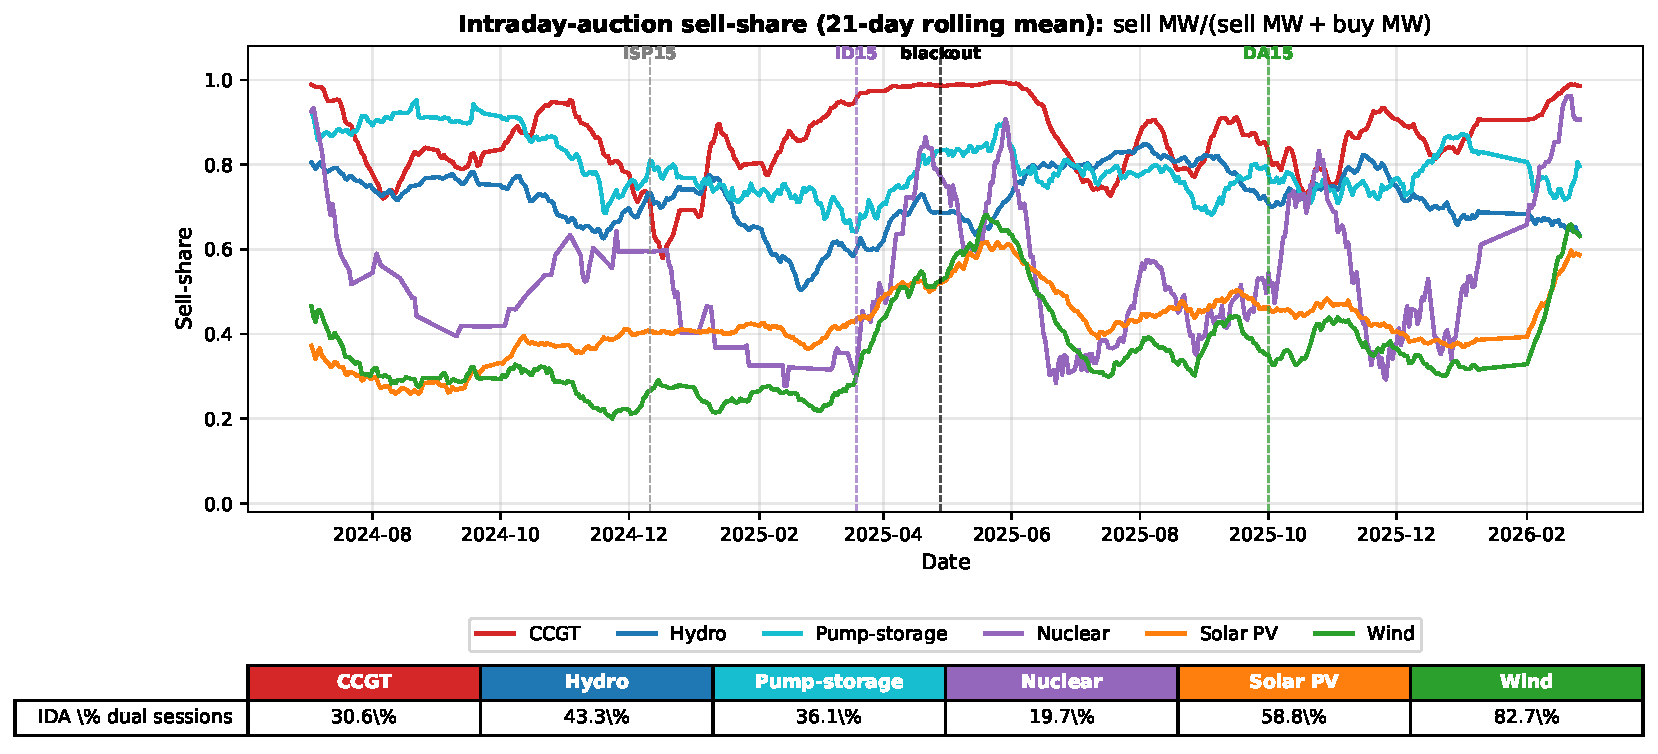
\includegraphics[width=\textwidth]{fig_sell_share_over_time.pdf}
\caption{\textbf{Intraday-auction sell-share by tech, 21-day rolling mean.} The ID15 cutover (2025-03-19) lifts the sell-share for nuclear, wind and pump-storage from near zero into the $0.3$-$0.5$ range; CCGT and hydro stay sell-dominant throughout. Vertical dashes: ISP15, ID15, blackout, DA15. The \%-dual mini-table reports the share of unit-sessions in which the unit submits both sell and buy offers.}
\label{fig:sell-share-over-time}
\end{figure}

The \%-dual row confirms an arbitrageur agent of the kind the sequential-market theory presupposes is empirically operating on the intraday bid stack across every production technology actually clearing volume --- the empirical confirmation of P7 (\S\ref{sec:theory:speaks}).


\subsection{Q3 (quantity-shift evidence) --- IDA in-band sell-share rises at ID15 (Spec A)}\label{sec:results:6-6b}
\phantomsection\label{tab:bsts-buy-share}

\emph{Takeaway.} ID15 transforms what the intraday auction is FOR. Before the reform, a unit holding nuclear or wind output used the IDA mainly to rebalance against forecast updates --- a one-way buy story. After ID15, units start using the IDA to also SELL output at per-quarter prices, capturing within-hour rent that the hourly grid did not let them price. Nuclear and wind show large sell-share rises (Table~\ref{tab:bsts-spec-a}).

\paragraph{Mechanism.} The mechanism is the spot-side ladder-widening of \S\ref{sec:theory:id15}(M4) read on the participation margin: rather than expanding the steps of a single curve, units enter the IDA on the sell side that previously did not bid there at all. We cannot run a same-calendar 2024 placebo because the pre-IDA-reform sell-share was almost a constant; the falsification is the descriptive break of Figure~\ref{fig:sell-share-over-time}.


\subsection{Q3 (quantity-shift evidence) --- bid-shape widening in critical hours (Spec C)}\label{sec:results:6-1}

\emph{Takeaway.} The granularity reform hands each firm a new tool: within each hour it can now place four quarter-prices instead of one. Do firms use it? Yes, on the day-ahead side. At ID15 combined-cycle gas restructures its day-ahead curve in critical hours by anticipation --- aggressive low-MW climb, steeper average slope, concave bend --- pure within-hour price discrimination via backward induction from the four IDA quarter-prices. At DA15, when both auctions become quarter-hourly, the CCGT day-ahead curve translates up, flattens on average, and bends convex --- the Cournot scale-up signature. Demand-side buyers raise their reservation prices in step. Both findings are robust to a long-pre window with year, month, and renewable controls, and to a regression-adjustment DiD under conditional parallel trends (\S\ref{sec:5-long-pre-ra}).

\begin{center}
\footnotesize
\setlength{\tabcolsep}{4pt}
\begin{tabular}{l l c c c c}
\toprule
                                 &              & \multicolumn{2}{c}{\textbf{ID15}} & \multicolumn{2}{c}{\textbf{DA15}} \\
\cmidrule(lr){3-4} \cmidrule(lr){5-6}
\textbf{Outcome (DiD $\theta$)} & \textbf{Tech} & DA & IDA & DA & IDA \\
\midrule
$\sigma_p$ (EUR/MWh)                 & CCGT          & $\mathbf{+4.17}^{***}$ & $+0.10$            & $\mathbf{+0.68}^{***}$  & $-0.68^{*}$ \\
                                     & Hydro         & $-0.53^{*}$            & $+0.43^{*}$        & $\mathbf{+1.80}^{***}$  & $+0.30$ \\
                                     & Pump-storage  & $\mathbf{-0.73}^{***}$ & $-0.01$            & $\mathbf{+0.92}^{***}$  & $+0.32^{*}$ \\
$\hat\alpha$ (EUR/MWh)               & CCGT          & $\mathbf{-40.2}^{***}$ & $11.8^{*}$         & $\mathbf{28.3}^{***}$   & $6.0^{**}$ \\
                                     & Hydro         & $0.2$                  & $87.3$             & $19.7$                  & $\mathbf{9.3}^{***}$ \\
                                     & Pump-storage  & $1.1$                  & $-3.0$             & $-1.8$                  & $16.1$ \\
$\hat\beta$ (EUR/MWh per MW)         & CCGT          & $\mathbf{0.27}^{***}$  & $-0.88^{*}$        & $\mathbf{-0.15}^{***}$  & $0.20$ \\
                                     & Hydro         & $0.15$                 & $-1.50$            & $\mathbf{-1.79}^{***}$  & $-0.01$ \\
                                     & Pump-storage  & $-0.01$                & $0.07$             & $0.01$                  & $-0.25$ \\
$\hat\gamma$ ($\times 10^{3}$)       & CCGT          & $\mathbf{-3.99}^{***}$ & $10.0$             & $\mathbf{1.03}^{***}$   & $7.6$ \\
                                     & Hydro         & $-305$                 & $-109$             & $\mathbf{-7{,}494}^{***}$ & $1.6$ \\
                                     & Pump-storage  & $0.07$                 & $1.45$             & $0.05$                  & $-0.16$ \\
$\text{HHI}_p$                       & CCGT          & $\mathbf{-0.076}^{***}$ & $\mathbf{-0.041}^{***}$ & $\mathbf{-0.059}^{***}$ & $\mathbf{+0.051}^{***}$ \\
                                     & Hydro         & $+0.004$               & $\mathbf{-0.049}^{***}$ & $+0.003$                & $\mathbf{+0.041}^{***}$ \\
                                     & Pump-storage  & $-0.023^{*}$           & $\mathbf{-0.040}^{**}$  & $+0.015$                & $-0.016$ \\
\bottomrule
\end{tabular}
\captionof{table}{\textbf{Spec~C per-curve DiD on bid-shape outcomes.} Critical-flat DiD on the five bid-shape statistics: price dispersion $\sigma_p$, intercept $\hat\alpha$, linear slope $\hat\beta$, curvature $\hat\gamma$, and bid-stack concentration $\text{HHI}_p$. Tight pre/post windows (reforzada held constant): ID15 pre 2024-12-19 to 2025-03-18, post 2025-03-19 to 2025-04-27 (40 days, pre-blackout); DA15 pre 2025-07-01 to 2025-09-30, post 2025-10-01 to 2025-12-31 (both post-blackout, reforzada active on both sides). Bandwidth $\delta = p_{90}-p_{50}$ window-specific. SEs clustered by date. A negative HHI DiD means the bid stack \emph{deconcentrates} (MW spreads across more tranches) in critical hours relative to flat. Robustness battery (long-pre with year + month + renewable controls, plus regression-adjustment DiD under conditional parallel trends) is in \S\ref{sec:5-long-pre-ra}. The ID15 DA CCGT (anticipation) cell and the DA15 DA CCGT cell are the retained headline cells: both have $\sigma_p > 0$ at $p<0.01$ and the $(\hat\alpha,\hat\beta,\hat\gamma)$ joint signature decomposes the shape change. ID15 IDA CCGT (small $\hat\alpha$, weakly significant $\hat\beta$, null $\sigma_p$) involves units largely out of the IDA pre-reform; we read it as suggestive.}
\label{tab:spec-c}
\end{center}

\paragraph{Parallel-trends robustness.} The headline DiD uses a tight pre-window so flat hours of the same season serve as a credible local control for critical hours. A same-calendar 2024 placebo (cutover shifted one year earlier) gives a sign-opposite placebo on $\sigma_p$, so the placebo correction strengthens the reform-attributable shift. A long-pre window with year FE, calendar-month FE, and renewable-by-hour-class controls, plus a regression-adjustment DiD per \citet{heckman1997} under conditional parallel trends, deliver the same retained verdict on the headline ID15 DA CCGT and DA15 DA CCGT cells (\S\ref{sec:5-long-pre-ra}).

\paragraph{Reading the joint signature.} The geometry of the bid curve becomes legible only when price dispersion, level, slope, and curvature are read together. The robust price-side anchor $\sigma_p$ is significantly positive in both retained CCGT cells (DA15 DA $+0.68^{***}$ EUR/MWh; ID15 DA $+4.17^{***}$ EUR/MWh): the dispersion of in-band bid prices increases in critical hours relative to flat hours under each reform. The $(\hat\alpha, \hat\beta, \hat\gamma)$ decomposition then tells us \emph{how} the curve moved to deliver that extra price spread, and $\text{HHI}_p$ reads tranche concentration. Three stories emerge from Table~\ref{tab:spec-c}; Figure~\ref{fig:bidshape-shifts} visualises them.

\smallskip
\noindent
\textbf{DA15 day-ahead CCGT --- Cournot scale-up.} The curve translates up, flattens on average, and bends convex. The convex bend is the diagnostic piece: locally flat at low MW and locally steep at high MW. Read in the Cournot frame, this is more capacity placed at the competitive end of the stack (the scale-up of \S\ref{sec:theory:da15}(iv)) with a steeper marginal climb (the forward-side ladder widening of \S\ref{sec:theory:da15}(iii)) bundled into the same curve. The signature survives wider bandwidths (Table~\ref{tab:bandwidth-robustness}); a small same-sign pre-trend (Table~\ref{tab:pretrend-placebo}) means we read the reform window as continuation-and-augmentation rather than as a clean jump.

\smallskip
\noindent
\textbf{ID15 day-ahead CCGT (anticipation) --- pure price discrimination.} The curve translates down, steepens on average, and bends concave: an aggressive climb at low MW with a flatter tail. With the day-ahead still hourly, no scale-up is possible --- the only available margin is to discriminate within-hour using the four IDA quarter-prices via backward induction. That the same (tech, market) cell shows opposite curvature signs at the two reforms is direct evidence that the same firm responds with two distinct mechanisms (the Stage-1 option-value channel of \S\ref{sec:theory:da15}(v)).


\begin{figure}[h]
\centering
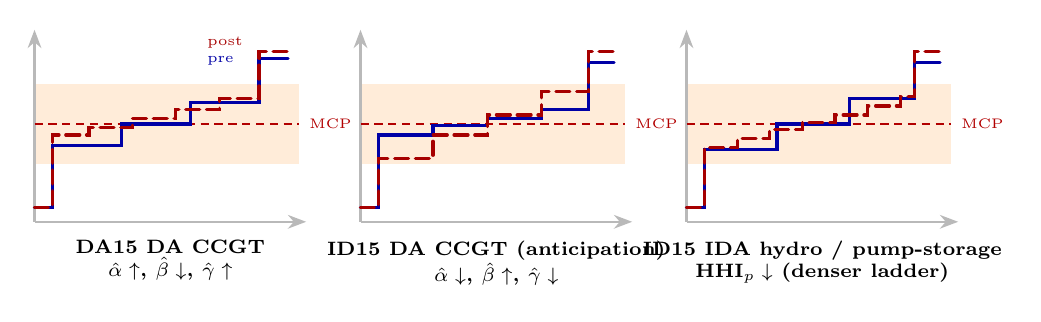
\begin{tikzpicture}[scale=0.46, every node/.style={font=\scriptsize}]
  \def\W{7.5}\def\H{5.0}\def\PMCP{2.7}\def\DELTA{1.1}
  \tikzset{
    axis/.style={draw=gray!55, thick, ->, >=Stealth},
    mcp/.style={red!70!black, thick, dash pattern=on 3pt off 2pt},
    band/.style={fill=orange!15},
    pre/.style={blue!65!black, very thick, line cap=round},
    post/.style={red!65!black, very thick, dash pattern=on 5pt off 2.5pt, line cap=round},
    plabel/.style={font=\scriptsize\bfseries, anchor=north, align=center},
  }
  %% Panel A: DA15 DA CCGT (slope flatter + intercept up, gamma convex)
  \begin{scope}[xshift=0cm, yshift=0cm]
    \fill[band] (0,\PMCP-\DELTA) rectangle (\W-0.2,\PMCP+\DELTA);
    \draw[axis] (0,0) -- (\W,0); \draw[axis] (0,0) -- (0,\H+0.3);
    \draw[mcp] (0,\PMCP) -- (\W-0.2,\PMCP);
    \node[red!70!black, anchor=west, font=\tiny] at (\W-0.18,\PMCP) {MCP};
    \draw[pre] (0,0.4) -- (0.5,0.4) -- (0.5,2.1) -- (2.4,2.1) -- (2.4,2.7) -- (4.3,2.7) -- (4.3,3.3) -- (6.2,3.3) -- (6.2,4.5) -- (7.0,4.5);
    \draw[post] (0,0.4) -- (0.5,0.4) -- (0.5,2.4) -- (1.5,2.4) -- (1.5,2.6) -- (2.7,2.6)
      -- (2.7,2.85) -- (3.9,2.85) -- (3.9,3.1) -- (5.1,3.1) -- (5.1,3.4) -- (6.2,3.4) -- (6.2,4.7) -- (7.0,4.7);
    \node[plabel] at (\W/2,-0.25) {\textbf{DA15 DA CCGT} \\ $\hat\alpha\uparrow$, $\hat\beta\downarrow$, $\hat\gamma\uparrow$};
    \node[blue!65!black, anchor=west, font=\tiny] at (4.5,4.45) {pre};
    \node[red!65!black, anchor=west, font=\tiny] at (4.5,4.95) {post};
  \end{scope}
  %% Panel B (was C): ID15 DA CCGT (anticipation: slope steeper + intercept down + gamma concave)
  \begin{scope}[xshift=9cm, yshift=0cm]
    \fill[band] (0,\PMCP-\DELTA) rectangle (\W-0.2,\PMCP+\DELTA);
    \draw[axis] (0,0) -- (\W,0); \draw[axis] (0,0) -- (0,\H+0.3);
    \draw[mcp] (0,\PMCP) -- (\W-0.2,\PMCP);
    \node[red!70!black, anchor=west, font=\tiny] at (\W-0.18,\PMCP) {MCP};
    \draw[pre] (0,0.4) -- (0.5,0.4) -- (0.5,2.40) -- (2.0,2.40) -- (2.0,2.65) -- (3.5,2.65) -- (3.5,2.85) -- (5.0,2.85) -- (5.0,3.10) -- (6.3,3.10) -- (6.3,4.4) -- (7.0,4.4);
    \draw[post] (0,0.4) -- (0.5,0.4) -- (0.5,1.75) -- (2.0,1.75) -- (2.0,2.40) -- (3.5,2.40) -- (3.5,2.95) -- (5.0,2.95) -- (5.0,3.60) -- (6.3,3.60) -- (6.3,4.7) -- (7.0,4.7);
    \node[plabel] at (\W/2,-0.25) {\textbf{ID15 DA CCGT (anticipation)} \\ $\hat\alpha\downarrow$, $\hat\beta\uparrow$, $\hat\gamma\downarrow$};
  \end{scope}
  %% Panel C: ID15 IDA hydro/pump-storage (HHI_p down, slope similar)
  \begin{scope}[xshift=18cm, yshift=0cm]
    \fill[band] (0,\PMCP-\DELTA) rectangle (\W-0.2,\PMCP+\DELTA);
    \draw[axis] (0,0) -- (\W,0); \draw[axis] (0,0) -- (0,\H+0.3);
    \draw[mcp] (0,\PMCP) -- (\W-0.2,\PMCP);
    \node[red!70!black, anchor=west, font=\tiny] at (\W-0.18,\PMCP) {MCP};
    \draw[pre] (0,0.4) -- (0.5,0.4) -- (0.5,2.0) -- (2.5,2.0) -- (2.5,2.7) -- (4.5,2.7) -- (4.5,3.4) -- (6.3,3.4) -- (6.3,4.4) -- (7.0,4.4);
    \draw[post] (0,0.4) -- (0.5,0.4) -- (0.5,2.05) -- (1.4,2.05) -- (1.4,2.30) -- (2.3,2.30) -- (2.3,2.55) -- (3.2,2.55)
      -- (3.2,2.75) -- (4.1,2.75) -- (4.1,2.95) -- (5.0,2.95) -- (5.0,3.20) -- (5.9,3.20) -- (5.9,3.45) -- (6.3,3.45) -- (6.3,4.7) -- (7.0,4.7);
    \node[plabel] at (\W/2,-0.25) {\textbf{ID15 IDA hydro / pump-storage} \\ $\text{HHI}_p\downarrow$ (denser ladder)};
  \end{scope}
\end{tikzpicture}
\caption{\textbf{Stylised retained bidding shifts.} Three in-band ladder reshapes observed in the data: DA15 day-ahead CCGT (level up, slope flatter, convex bend); ID15 day-ahead CCGT anticipation (level down, steeper, concave bend); ID15 intraday-auction hydro and pump-storage (denser ladder, level and slope unchanged). Blue solid: pre-reform; red dashed: post-reform.}
\label{fig:bidshape-shifts}
\end{figure}


\subsection{Synthesis --- aggregator vs strategic-bidder footprint by reform}\label{sec:results:6-5}\phantomsection\label{sec:results:synthesis}

\emph{Takeaway.} A useful way to read the empirical pattern across the two reforms is to ask \emph{which agent} the reform engages. The model has two: an aggregator (price-taker, hedges its own forecast error) and a strategic bidder (residual monopolist, discriminates against demand uncertainty). The aggregator's footprint should be biggest at the SPOT reform, because the gain from a finer spot scales with within-hour forecast variance. The strategic bidder's footprint should be biggest at the FORWARD reform, because that is when the bidder gets per-product residual demand on the leg it controls. The data deliver exactly this split: ID15 surfaces the aggregator (IDA sell-share rise, wedge SD that does not collapse); DA15 surfaces the strategic bidder (CCGT day-ahead ladder widening). The pricing chain of \S\ref{sec:results:6-3} ties the two together. Per-firm residual-demand thickens for every dominant firm, markup compresses by the Cournot first-order condition, and clearing prices fall on both reform-side legs.


% =====================================================================
\section{Conclusion: granularity is a strategic-latitude reveal, not a market-power amplifier}\label{sec:conclusion}
% =====================================================================

\emph{Headline.} A market-microstructure reform that moves the trading clock from hour to quarter acts as a \emph{strategic-latitude reveal}, not a technology shock. Marginal costs, capacity, and the set of participants are unchanged. What changes is the within-hour room each agent has to discriminate, arbitrage, and hedge. The equilibrium response traces exactly that --- combined-cycle gas restructuring its day-ahead ladder in critical hours, intraday hydro and pump-storage adding tranche density, demand-side buyers raising their reservation prices in step, and operational aggregators using the finer grid to manage imbalance.

\paragraph{Does granularity amplify market power?} The dimensions where we have robust identification go the opposite way. The scarcity wedge between day-ahead and intraday prices is positive in every regime, so the standing rent does not vanish under the reform; what changes is the within-hour distribution. The model's pricing primitive points the same way: per-firm residual demand becomes more elastic post-reform for every one of the four dominant CCGT-owning firms, with direction and significance surviving a long-pre window with year and month controls though magnitude shrinks roughly in half (Appendix~\ref{app:robustness}.10). The Cournot first-order condition then implies markup compression, and the BSTS clearing-price effect is negative on both reform-side legs. None of the robust findings shows widening of the strategic margin.

\paragraph{Does it harm consumers?} Net of the post-blackout regulatory regime, no. Across the reform sequence the real-time redispatch and aFRR channels fall while the pre-real-time Fase~I channel rises (Figure~\ref{fig:efficiency_gains}); the bulk of the real-time decrease appears to be a procurement-timing displacement from real-time to Fase~I inside the post-blackout regime, not a granularity-driven efficiency gain --- the expert at NeuroEnerg\'ia explicitly predicted no granularity-side effect on ajuste costs because banda secundaria and the PBF technical restrictions stay hourly and real-time was already quarter-hourly. What our identification does pin to the granularity reform is the regulatory imbalance penalty per absolute MWh of deviation: the BS3 cost-sharing per MWh drops by about a third at the March cutover, with respect to a counterfactual that controls for renewables and gas prices, while the system's aggregate imbalance volume is statistically unchanged. The reform reorganises the within-hour composition of imbalance; the marginal cost of clearing the residual falls; the level of forecast errors does not. The CO\textsubscript{2} damage cost of the reforzada-driven redispatch \citep{davi_arderius_graf_2026} is a separate welfare component our framework does not compute; it should be netted against the granularity-side saving in any full social-cost accounting.

\paragraph{Is ID15 implicated in the April 2025 blackout?} The evidence does not support a direct attribution, but it sharpens a question worth flagging. Three facts in the open. First, REE's post-blackout response is technology-specific: combined-cycle gas roughly doubles in restriction dispatch while solar and hydro are curtailed, a voltage-support stance rather than a market-driven outcome. Second, the spring renewable supply was nearly the same in 2024 and 2025, yet only 2025 blacked out --- so the cleanest systemic change between the two springs is the MTU15 sequence. Third, in the 40 days between ID15 and the blackout, nuclear's auction-plus-bilateral output drops sharply against a same-calendar 2024 placebo and is absent in the post-blackout DA15 window (Appendix~\ref{app:robustness}.8). One plausible chain: ID15 sharpens bidding on the granular leg, day-ahead prices run very low on solar-heavy days, and inflexible nuclear baseload (which carries the bulk of synchronous inertia) loses room to operate. Each step is testable. None alone identifies the blackout's causal trigger, and the ENTSO-E Expert Panel \citep{entsoe_blackout_iberia_2026} does not list ID15 as a contributing factor --- the panel's root-cause tree is voltage- and reactive-power-control, not market microstructure.

Anecdotally, the parallel CNMC report does flag the move to quarter-hourly trading as one contributor to the abrupt voltage variations observed in the months around the incident \citep[p.~44]{cnmc_blackout_recommendations_2026}:
\begin{quote}
\itshape It is worth recalling that the implementation of the 15-minute trading unit in the Spanish intraday market was completed on 18 March 2025, one month before the incident, with the entry into force of quarter-hourly trading in both the intraday auctions and the continuous intraday market. The implementation was carried out within the framework of the European intraday coupling projects in line with Regulation (EU) 2017/2195. The evolution to quarter-hourly trading and settlement has made the appearance of transitions between negative and positive prices increasingly frequent, leading to strong changes in production volumes in certain zones.\footnote{Original (CNMC report, p.~44): \emph{``A este respecto, cabe recordar que el proceso de implantaci\'on de la unidad de negociaci\'on de 15 minutos en el mercado intradiario espa\~nol se complet\'o el 18 de marzo de 2025, 1 mes antes del incidente, con la entrada en vigor de la negociaci\'on cuarto-horaria tanto en las subastas intradiarias como en el mercado intradiario continuo. La implementaci\'on se realiz\'o en el marco de los proyectos europeos de acoplamiento intradiario en coherencia con el Reglamento (UE) 2017/2195. La evoluci\'on a una negociaci\'on y liquidaci\'on de productos cuarto horarios ha hecho cada vez m\'as frecuente la aparici\'on de transiciones entre precios negativos y positivos que conducen a fuertes cambios del volumen de producci\'on en determinadas zonas.''}}
\end{quote}

Answering whether market-microstructure reforms contributed to the macro-conditions that made the proximate triggers cascade --- frequent within-hour swings, converter-driven volatility under fixed-power-factor renewable dispatch --- is beyond this thesis's scope and requires electrical-engineering knowledge we do not bring. The CNMC's flag points exactly at that gap.

\newpage

\bibliographystyle{plainnat}
\addcontentsline{toc}{section}{References}
\bibliography{references}

\newpage

% Drop subsections (and below) from the TOC for the appendix.
\addtocontents{toc}{\protect\setcounter{tocdepth}{1}}

\appendix

% =====================================================================
\section{Robustness}\label{app:robustness}
% =====================================================================

\subsection{Year-by-year solar coefficient: the renewable response is non-stationary}\label{app:solar-year-coefs}

The Spec~A BSTS uses long pre-windows (2022 onwards) with $\text{wind}_t\times\mathbf{1}\{\text{year}=y\}$ and $\text{solar}_t\times\mathbf{1}\{\text{year}=y\}$ interactions. The economic reason is that Spanish wind+solar installed capacity grew by a factor of $\sim 6$ over 2018-2025, and the marginal effect of an additional GWh of renewable output on price is not constant across that period. A flat-coefficient spec mis-fits the cross-year merit-order shift and reports artificially confident treatment effects (\S\ref{sec:empirical:specA}).

Table~\ref{tab:solar-year-coefs} reports the cumulative solar coefficient (base + year-dummy) by calendar year, extracted from the BSTS posterior of the price spec under both windows (ID15 pre ends 2025-03-18, DA15 pre ends 2025-09-30). \textbf{Conditional posterior means} (the coefficient when the spike-and-slab includes the regressor). The wind base coefficient is stable around $-0.50$ EUR/MWh per GWh; the wind$\times$year interactions all have inclusion probability below $1.5\%$. The solar coefficient is the one that varies.

\begin{center}
\footnotesize
\setlength{\tabcolsep}{7pt}
\begin{tabular}{l c c c}
\toprule
\textbf{Year} & \textbf{ID15 IDA spec} & \textbf{DA15 IDA spec} & \textbf{DA15 DA spec} \\
\midrule
2022 (base)   & $-0.22$ & $-0.23$ & $-0.22$ \\
2023          & $-0.02$ & $-0.23$ & $-0.17$ \\
2024          & $\mathbf{-0.46}$ & $\mathbf{-0.47}$ & $\mathbf{-0.40}$ \\
2025\, $^{\dagger}$ & $\mathbf{-0.29}$ \emph{(Jan-Mar only on ID15)} & $\mathbf{-0.50}$ & $\mathbf{-0.49}$ \\
\midrule
\multicolumn{4}{l}{\emph{Implied weighted average for the post-window prediction}} \\
2024+2025 weighted avg $^{\ddagger}$ & $-0.43$ & $-0.45$ & $-0.44$ \\
\bottomrule
\end{tabular}
\captionof{table}{\textbf{Cumulative solar coefficient (EUR/MWh per GWh of solar) by year}, extracted from the BSTS posterior of the corresponding price spec. Cumulative coefficient = base $+$ year-dummy interaction, conditional posterior mean among MCMC draws that include the regressor. $^{\dagger}$The ID15 spec pre-window ends 2025-03-18, so its 2025-by-solar coefficient is fitted on Jan-Mar 2025 only, when Spanish solar production is at its lowest seasonal level; the DA15 spec pre-window extends through 2025-09-30 and includes summer, giving the more representative estimate. $^{\ddagger}$Months-weighted average of the 2024 and 2025 cumulative coefficients (12 months of 2024 + available months of 2025): this is the coefficient one would extrapolate forward if 2024 and 2025 were pooled into a single dummy for the post-window prediction; the per-year BSTS instead extrapolates using the 2025-row coefficient alone.}
\label{tab:solar-year-coefs}
\end{center}

Reading the table: the DA15 spec (which sees Jan-Sep 2025) tells the cleaner story. Solar's marginal price-suppressing effect is roughly constant from 2022 to 2023, then nearly doubles from 2023 to 2024 (Spain added $\sim\!5$ GW of solar capacity in 2024 alone), and continues to deepen in 2025 as solar saturates more clock-hours and negative-price events become routine. The ID15 spec's 2025 coefficient looks deceptively small (Jan-Mar winter sun is weak) but the underlying renewable response in 2025 is the most negative on record. The non-stationarity is exactly what the year interaction is designed to absorb: a flat-coefficient spec would average $-0.22$ (2022) and $-0.50$ (2025) into a single value around $-0.35$, mis-fitting both ends of the window.

\paragraph{Calibrated-solar robustness: how much of the price drop is solar vs the reform?} A natural concern about the headline BSTS counterfactual is that Spanish solar capacity grew rapidly through 2024 and 2025, so the marginal price-suppressing effect of solar is itself non-stationary. The BSTS per-year spike-and-slab attempts to capture this via year-by-solar interactions; the conditional posterior means (Table~\ref{tab:solar-year-coefs}) are $-0.46$ for 2024 and $-0.29$ for the Jan-Mar-2025 sample on the ID15 spec, suggesting a strong solar effect that may not be fully credited in the post-window prediction. If the post-window counterfactual under-credits solar, the residual ``price drop'' that we attribute to the reform is partly mechanical (it is the solar effect we failed to attribute correctly). We therefore implement a \textbf{calibrated-solar counterfactual}: pre-subtract a known solar contribution $\beta^{\text{cal}}_{\text{solar}} \cdot \text{solar}_t \cdot \mathds{1}\{t \ge 2024\}$ from observed prices, fit the BSTS state-space model on the residual (with the usual base regressors but no year interactions), and add the calibrated solar contribution back to the post-window prediction before computing the treatment effect.

\begin{center}
\footnotesize
\setlength{\tabcolsep}{6pt}
\begin{tabular}{l r r r r r r}
\toprule
& \multicolumn{3}{c}{\textbf{ID15 IDA}} & \multicolumn{3}{c}{\textbf{DA15 DA}} \\
\cmidrule(lr){2-4} \cmidrule(lr){5-7}
\textbf{Calibrated solar coefficient $\beta^{\text{cal}}_{\text{solar}}$ (EUR/MWh per GWh)} & \textbf{Real} & \textbf{Placebo} & \textbf{Net} & \textbf{Real} & \textbf{Placebo} & \textbf{Net} \\
\midrule
$-0.21$ (BSTS unconditional default)                   & $-41$ & $+32$ & $\mathbf{-73}$ & $+30$ & $+43$ & $-13$ \\
$-0.29$ (per-year cond.\ 2025, ID15 spec)              & $-38$ & $+36$ & $\mathbf{-74}$ & $+21$ & $+32$ & $-12$ \\
$-0.40$ (per-year cond.\ 2024, DA15 DA spec)           & $-30$ & $+36$ & $\mathbf{-66}$ & $+18$ & $+27$ & $-10$ \\
$\mathbf{-0.46}$ (per-year cond.\ 2024, ID15 spec)     & $-26$ & $+37$ & $\mathbf{-63}$ & $+9$  & $+23$ & $-13$ \\
$-0.50$ (per-year cond.\ 2025, DA15 spec)              & $-23$ & $+37$ & $\mathbf{-60}$ & $+9$  & $+19$ & $-10$ \\
\bottomrule
\end{tabular}
\captionof{table}{\textbf{Calibrated-solar BSTS treatment effects on clearing price.} EUR/MWh; $-0.46$ row uses the user's preferred ``trust the 2024 conditional'' substitution. The calibrated approach explicitly subtracts $\beta^{\text{cal}}_{\text{solar}} \cdot \text{solar} \cdot \mathbf{1}\{t \ge 2024\}$ from prices, fits BSTS on the residual (no year interactions), and adds the calibrated contribution back to the post-window prediction. Placebo column uses the same calibration but with the cutover shifted one year earlier (real reform absent in the placebo window). Real, placebo, and net all measured on the price level in EUR/MWh.}
\label{tab:calibrated-solar}
\end{center}

\textbf{The price drop at ID15 IDA survives every solar calibration we tried.} Under the most aggressive solar coefficient ($-0.50$, the DA15-spec conditional 2025 mean) the real-effect point estimate is $-23$ EUR/MWh; under the user's preferred ``trust the 2024 conditional'' value of $-0.46$ it is $-26$ EUR/MWh; under the BSTS unconditional default it is $-41$ EUR/MWh. After 2024-same-calendar placebo-netting (which absorbs whatever cross-season variation exists in the spring window) the net effects are uniformly larger in magnitude ($-60$ to $-74$ EUR/MWh) because the placebo windows themselves have positive ``effects'' under the calibrated specification, reflecting whatever upward residual variation Spring 2024 carried. The DA15 DA real effect is essentially null across all solar calibrations ($+9$ to $+30$ EUR/MWh, $\approx 0$); the net effect is mildly negative ($-10$ to $-13$ EUR/MWh) under every solar calibration but the magnitude is much smaller than at ID15 and the credible intervals always bracket zero.

\textbf{Bottom line.} The ID15 IDA price drop is robustly negative in sign and substantial in magnitude under every solar coefficient we could justify. Solar's strong 2024 marginal effect ($-0.46$) does not explain the ID15 price drop --- the reform did something to the granular leg's clearing price on top of what solar alone would predict. The DA15 DA effect is small to null under every calibration. We treat the ID15 drop as a real reform effect and the DA15 drop as not separately identified. The per-firm slope-thickening result (Appendix~\ref{app:robustness}.10) remains the cleanly-identified pricing-chain INPUT and is unaffected by this discussion.

\paragraph{OLS cross-check.} The wide credible intervals in the calibrated-solar BSTS reflect the state-space level component's flexibility, which absorbs persistent low-frequency variation that the regression then has no way to pin down. We complement the BSTS with a standard OLS regression on the same daily price panel, including calendar-month and day-of-week fixed effects (the seasonal structure that BSTS encoded via local-level + 7-day seasonal), a time trend (linear or quadratic), gas price, and per-year wind and solar interactions. Standard errors are Newey-West HAC with $7$-day bandwidth to account for daily price autocorrelation. The model:
\[
p_t \;=\; \alpha + \theta\,\text{POST}_t + \beta_{\text{wind}}\text{wind}_t + \beta_{\text{solar}}\text{solar}_t + \beta_{\text{gas}}\text{gas}_t + \sum_y \gamma_y\,\text{renew}_t \cdot \mathds{1}\{\text{year}=y\} + \phi_m + \delta_{\text{dow}} + g(t) + \varepsilon_t.
\]

\begin{center}
\footnotesize
\setlength{\tabcolsep}{6pt}
\begin{tabular}{l r r r r}
\toprule
& \multicolumn{2}{c}{\textbf{ID15 IDA price}} & \multicolumn{2}{c}{\textbf{DA15 DA price}} \\
\cmidrule(lr){2-3} \cmidrule(lr){4-5}
\textbf{Specification (POST coef $\theta$)} & $\hat\theta$ & HAC SE & $\hat\theta$ & HAC SE \\
\midrule
Spec 1: base $+$ month FE $+$ DOW FE                 & $\mathbf{-31.7}^{***}$ & $8.2$ & $-8.3$           & $5.3$ \\
Spec 2: $+$ linear time trend                         & $\mathbf{-23.7}^{***}$ & $8.6$ & $+8.3$           & $7.3$ \\
Spec 3: $+$ year-by-renewable (per year)              & $\mathbf{-45.8}^{***}$ & $9.6$ & $-8.6$           & $8.1$ \\
Spec 4: $+$ year-by-renewable (2024+ pooled)          & $\mathbf{-38.7}^{***}$ & $7.3$ & $-4.6$           & $7.7$ \\
Spec 5: $+$ quadratic time trend                      & $\mathbf{-53.1}^{***}$ & $6.8$ & $\mathbf{-18.9}^{**}$ & $9.2$ \\
\bottomrule
\end{tabular}
\captionof{table}{\textbf{OLS price-effect estimates with full controls.} Daily clearing-price regressions with calendar-month and day-of-week fixed effects, gas price, time trend (linear or quadratic), and year-by-renewable interactions. Newey-West HAC standard errors with $7$-day bandwidth. POST = 1 on/after the reform cutover. Spec 4 (year-by-renewable with 2024+2025 pooled) implements the user-suggested fix for the Jan-Mar-2025-only-fit problem. $^{**}\,p<0.05$, $^{***}\,p<0.01$. ID15 IDA pre-window 2022-01-01 to 2025-03-18, post 2025-03-19 to 2025-04-27. DA15 DA pre 2022-01-01 to 2025-09-30, post 2025-10-01 to 2025-12-31.}
\label{tab:ols-price-full-controls}
\end{center}

\textbf{OLS verdict matches the calibrated-solar BSTS verdict.} The ID15 IDA price drop is significant at every standard significance level across all five specifications ($-24$ to $-53$ EUR/MWh, $p<0.01$ throughout). The DA15 DA effect ranges from $-4.6$ (null, $p=0.55$) to $-18.9$ (significant under quadratic trend, $p=0.04$); the bulk of specifications return small null or marginally-significant negative coefficients. OLS with full controls is more precise than the BSTS (smaller standard errors, narrower confidence intervals) but qualitatively delivers the same conclusion: \textbf{ID15 has a robust own-venue price drop; DA15 does not}.

This diagnostic also clarifies why several level findings (\S\ref{sec:results:6-3}) lose significance under the year-interaction spec: forecast uncertainty about what solar's marginal price impact will be in the post-cutover window is large precisely because the coefficient has been shifting fast in the years immediately preceding the cutover.



\paragraph{Note on bid-shape outcomes in this appendix.} The Spec~C robustness tables below report on the headline quintuple $(\sigma_p, \hat\alpha, \hat\beta, \hat\gamma, \text{HHI}_p)$ used in \S\ref{sec:data:bandwidth}. The cross-border and offer-type checks lead with $\sigma_p$ (the robust price-side anchor); for a near-linear curve $\sigma_p \approx |\hat\beta|\cdot\sigma_Q$, so the signs on those checks track $\hat\beta$ up to estimator noise (and via curvature track $\hat\gamma$).

\subsection{Pre-trend placebo}\label{sec:5b}
Split the pre-window at its midpoint and run the same DiD on the two halves; genuine reform effects should leave that placebo near zero. ID15 own-market cells pass cleanly (sign flips between real and placebo). The DA15 own-market CCGT placebo runs same-sign as the real, so the DA15 CCGT widening is continuation-plus-augmentation rather than a clean jump. Figure~\ref{fig:parallel-trends-sigma-p} is the visual analogue.

\begin{center}
\scriptsize
\setlength{\tabcolsep}{3pt}
\begin{tabular}{l c c c c c c c c}
\toprule
        & \multicolumn{2}{c}{\textbf{ID15 IDA (own)}} & \multicolumn{2}{c}{\textbf{ID15 DA (cross)}} & \multicolumn{2}{c}{\textbf{DA15 DA (own)}} & \multicolumn{2}{c}{\textbf{DA15 IDA (cross)}} \\
\cmidrule(lr){2-3} \cmidrule(lr){4-5} \cmidrule(lr){6-7} \cmidrule(lr){8-9}
\textbf{Tech} & Hdln & Plac & Hdln & Plac & Hdln & Plac & Hdln & Plac \\
\midrule
\multicolumn{9}{l}{\emph{Intercept $\alpha$ (EUR/MWh; positive = higher curve)}} \\
CCGT      & $11.8^{*}$           & $4.9$            & $-40.2^{***}$       & $1.8$            & $28.3^{***}$       & $40.2^{***}$ & $6.0^{**}$       & $3.8^{**}$ \\
Hydro     & $87.3$               & $10.2^{***}$     & $0.2$               & $-0.4$           & $19.7$             & $53.3^{*}$   & $9.3^{***}$      & $6.3^{***}$ \\
Pump-storage & $-3.0$            & $-12.7^{***}$    & $1.1$               & $1.3$            & $-1.8$             & $-4.3$       & $16.1$           & $-4.9$ \\
\addlinespace
\multicolumn{9}{l}{\emph{Slope $\beta$ (EUR/MWh per MW; more negative = steeper)}} \\
CCGT      & $-0.881^{*}$         & $0.146$          & $0.269^{***}$       & $0.004$          & $-0.150^{***}$     & $-0.206^{***}$ & $0.200$        & $-0.101$ \\
Hydro     & $-1.498$             & $-0.156^{**}$    & $0.154$             & $-1.703^{***}$   & $-1.785^{***}$     & $1.176^{***}$  & $-0.012$       & $-0.022$ \\
Pump-storage & $0.071$           & $0.248$          & $-0.010$            & $0.015^{*}$      & $0.008$            & $0.046^{***}$  & $-0.254$       & $0.007$ \\
\addlinespace
\multicolumn{9}{l}{\emph{Curvature $\gamma$ (EUR/MWh per MW$^2$; positive = convex)}} \\
CCGT      & $0.0100$             & $0.0334^{*}$     & $-0.0040^{***}$     & $0.0015^{***}$   & $0.0010^{***}$     & $0.0022^{***}$ & $0.0076$       & $0.0002$ \\
Hydro     & $-0.1088$            & $0.2455$         & $-0.3055$           & $-1.3947$        & $-7.4938^{***}$    & $1.6198$       & $0.0016$       & $-0.0105$ \\
Pump-storage & $0.0014$          & $0.0005$         & $0.0001$            & $0.0002$         & $0.0001$           & $0.0000$       & $-0.0002$      & $-0.0002$ \\
\bottomrule
\end{tabular}
\captionof{table}{\textbf{Pre-only midpoint placebo for Spec~C bid-shape DiD, all four (reform, market) cells.} Windows: ID15 pre 2024-12-19 to 2025-03-18 (midpoint placebo splits this at $\sim$2025-02-01); DA15 pre 2025-07-01 to 2025-09-30 (midpoint $\sim$2025-08-15). ``Hdln'' reproduces the headline DiD from \S\ref{sec:results:6-1} using the full pre/post split; ``Plac'' fits the same critical/flat DiD on the pre-window split at its midpoint (no reform crosses the midpoint, so ``Plac'' should be null under parallel trends). Stars: $^{*}p<0.1$, $^{**}p<0.05$, $^{***}p<0.01$.}
\label{tab:pretrend-placebo}
\end{center}

\paragraph{$\sigma_p$ as the rugged visualization.} For the parallel-trends figure we lead with $\sigma_p$ (Figure~\ref{fig:parallel-trends-sigma-p}) and report the structural decomposition $(\hat\alpha, \hat\beta, \hat\gamma, \text{HHI}_p)$ alongside (Figure~\ref{fig:parallel-trends-abgN}). $\sigma_p$ requires only price-side variation, is bounded in $[0,\delta]$, and is well-defined on single-tranche curves; the slope $\hat\beta$ needs joint $p$--$q$ variation and is noisier on sparse curves. For near-linear curves the two are related by $\sigma_p\approx|\hat\beta|\sigma_Q$, so the patterns track up to estimator noise.

\begin{figure}[h]
\centering
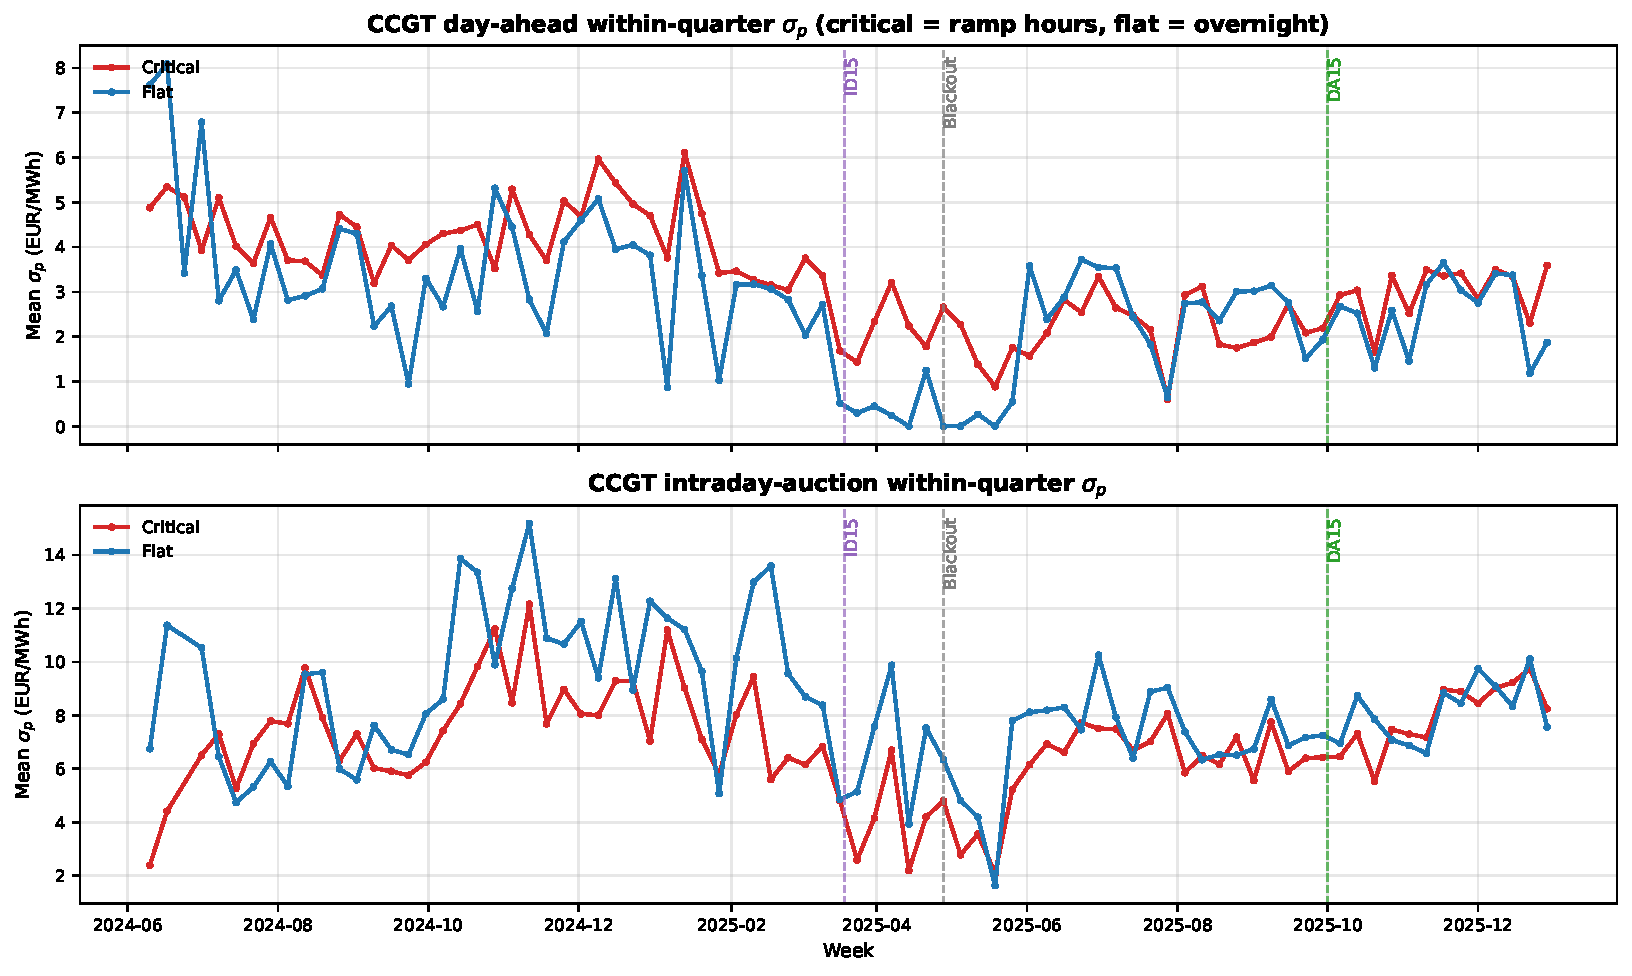
\includegraphics[width=\textwidth]{fig_parallel_trends_sigma_p.pdf}
\caption{\textbf{Headline parallel-trends diagnostic: weekly CCGT within-quarter $\sigma_p$ by hour-class, 2024-06 to 2025-12.} \emph{Top:} day-ahead; \emph{Bottom:} intraday-auction (latest-session in-band tranches, $|p_k - \text{MCP}| \le 50$~EUR/MWh). Red: critical hours; blue: flat hours. Vertical dashes: ID15 (2025-03-19), blackout (2025-04-28), DA15 (2025-10-01). $\sigma_p$ is the rugged price-side dispersion that visualizes the within-day reform effect without requiring $q$-side identification (cf.\ the structural decomposition in Figure~\ref{fig:parallel-trends-abgN}).}
\label{fig:parallel-trends-sigma-p}
\end{figure}

\begin{figure}[h]
\centering
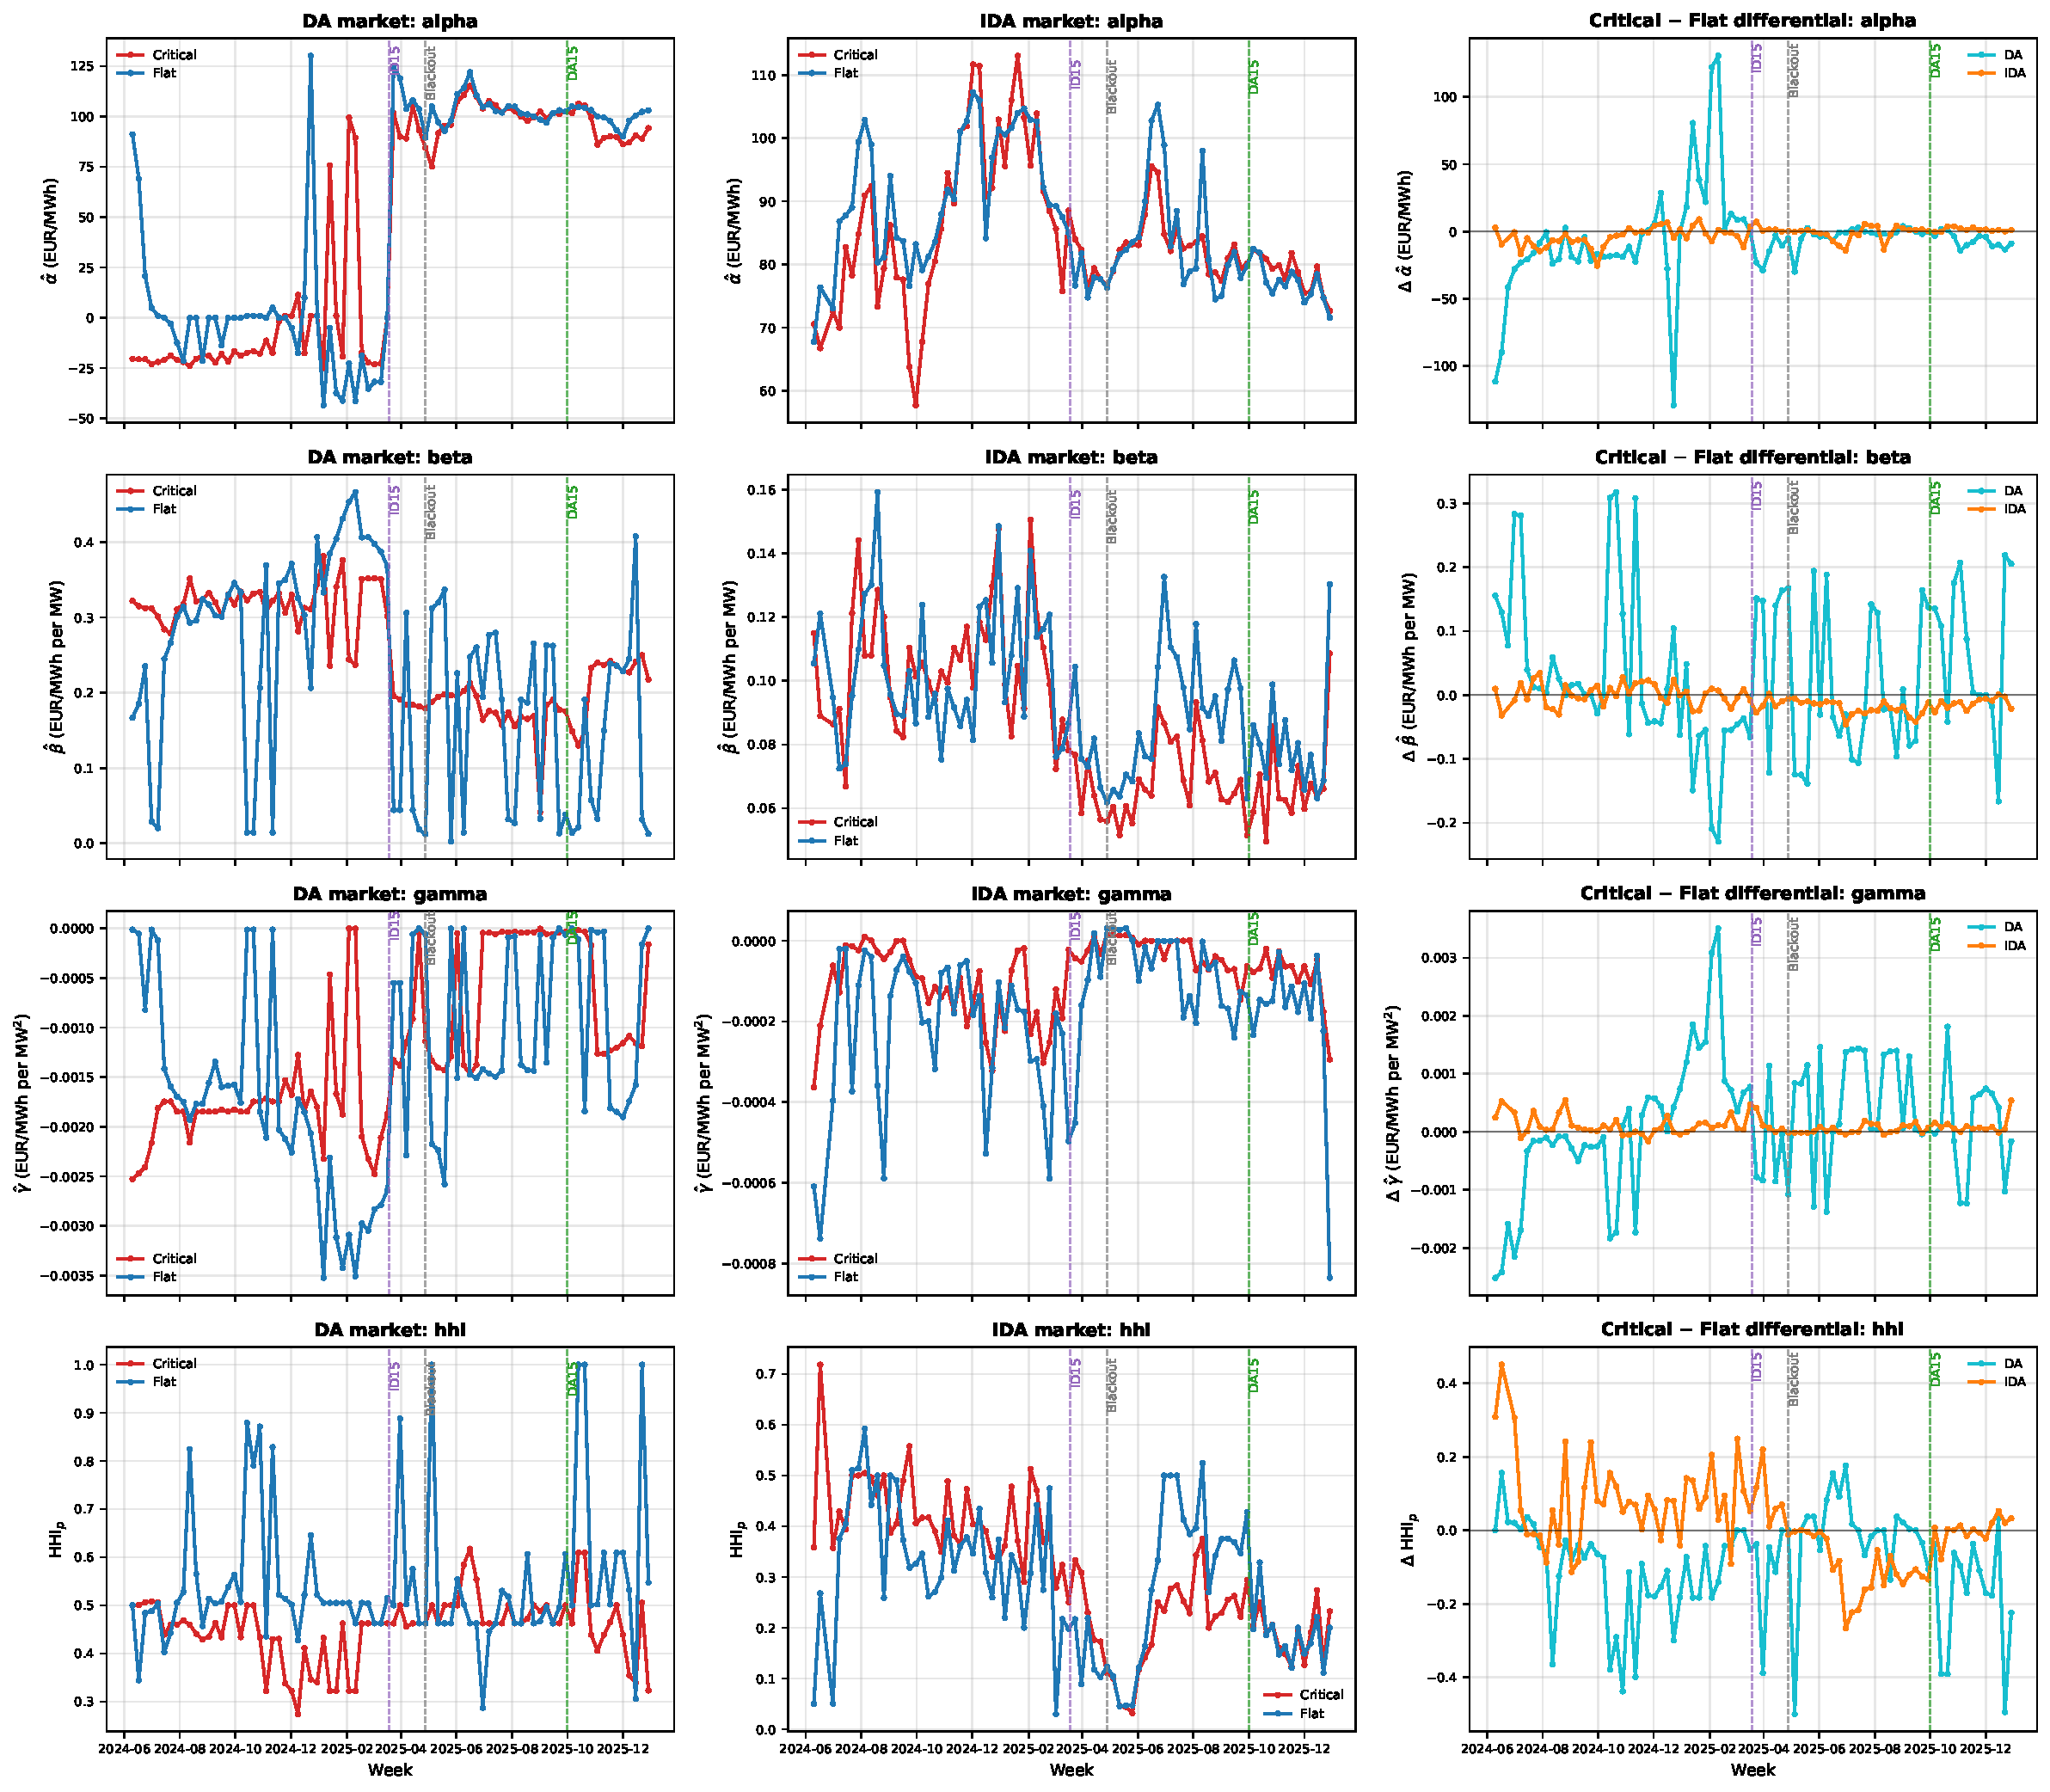
\includegraphics[width=\textwidth]{../../figures/thesis/fig_parallel_trends_abgN.pdf}
\caption{\textbf{Structural decomposition: weekly CCGT per-curve $\hat\alpha,\hat\beta,\hat\gamma,\text{HHI}_p$ by hour-class, 2024-06 to 2025-12.} \emph{Left column}: DA market levels by hour-class. \emph{Middle column}: IDA market levels. \emph{Right column}: critical $-$ flat differential by market (cyan DA, orange IDA), the visual analogue of the Spec~C DiD coefficient. In-band per-curve OLS quadratic fit at $\delta = 150$~EUR/MWh; per-cell aggregation uses the median across curves with $n_{\text{tranche}} \ge 4$ and $\Delta q \ge 20$~MW for the $\hat\beta$ and $\hat\gamma$ rows (joint $p$--$q$ identification floor); $\hat\alpha$ and $\text{HHI}_p$ have no such floor and use all curves. Vertical dashes mark the three reform dates. The $\text{HHI}_p$ row carries the cleanest visual signal (DA critical sits sustainedly below flat post-DA15, the visual signature of bid-stack deconcentration); $\hat\alpha$ is dominated by the spring-2025 shared negative-price shock; $\hat\beta$ and $\hat\gamma$ rows are noisier per the identification argument in the paragraph above and should be read in conjunction with the $\sigma_p$ panel of Figure~\ref{fig:parallel-trends-sigma-p}.}
\label{fig:parallel-trends-abgN}
\end{figure}

\subsection{Long-pre window with year/season/renewable controls and conditional parallel trends (RA-DiD)}\label{sec:5-long-pre-ra}

I extend the pre-window to 2022-01-01, add year FE, calendar-month FE, and crit$\times$wind/crit$\times$solar interactions; and as a separate spec run the regression-adjustment DiD of \citet{heckman1997} under conditional parallel trends. ID15 DA CCGT (anticipation) survives both checks on $\sigma_p$ and HHI; DA15 DA CCGT survives on $\sigma_p$, the HHI sign flips under RA-DiD so the $\sigma_p$ side is the rugged headline. Side technologies omitted: only cells that survive at least the long-pre spec are reported (Table~\ref{tab:spec-c-longpre-ra}).

\begin{center}
\footnotesize
\setlength{\tabcolsep}{6pt}
\begin{tabular}{l l c c c}
\toprule
\textbf{Cell}                       & \textbf{Outcome} & \textbf{Tight (1)} & \textbf{Long-pre + controls (2)} & \textbf{RA-DiD (3)} \\
\midrule
ID15 DA CCGT (anticipation)         & $\sigma_p$       & $+19.42^{***}$ & $+10.78^{***}$ & $+12.71^{**}$ \\
                                    & $\text{HHI}_p$   & $-0.076^{***}$ & $-0.098^{***}$ & $-0.000$ \\
\addlinespace
DA15 DA CCGT                        & $\sigma_p$       & $+1.25^{**}$   & $+5.47^{***}$  & $+1.72$ \\
                                    & $\text{HHI}_p$   & $-0.059^{***}$ & $-0.028^{***}$ & $+0.099^{**}$ \\
\addlinespace
\bottomrule
\end{tabular}
\captionof{table}{\textbf{Spec~C robustness: tight (1), long-pre with year+month+renewable controls (2), and regression-adjustment DiD per \citet{heckman1997} under conditional PT (3).} Windows match Table~\ref{tab:spec-c}. \emph{Bandwidth note:} this robustness uses the wider strategic bandwidth $H=140$ EUR/MWh of the underlying per-curve panel (the bandwidth of Figure~\ref{fig:parallel-trends-sigma-p}), not the window-specific $p_{90}$ of Table~\ref{tab:spec-c}; $\sigma_p$ scales with band width, so the magnitudes here are larger than in the headline table but the signs and significances on the headline cells are the comparable object. Spec (2) extends pre to 2022-01-01 and adds year FE, month FE, crit$\times$wind / crit$\times$solar interactions. Spec (3) regresses per-unit pre$\to$post change on average wind and solar on FLAT hours, predicts the counterfactual at critical units' covariates, ATT = realized $-$ predicted; bootstrap SEs 500 reps. Cells reported are those surviving at least spec (2).}
\label{tab:spec-c-longpre-ra}
\end{center}

\paragraph{Per-firm $b_{mt}$ under the same long-pre control.} I run the same long-pre + year + month FE on the per-firm $b_{mt}$ thickening: magnitude shrinks from the tight-window range $+13$\%--$+28$\% to $+8$\%--$+15$\% across the four dominant CCGT-owning firms, all firm cells still significant. Direction robust, magnitude roughly halved.

\subsection{Hour-class falsification (midday vs.\ flat)}\label{sec:5a}\phantomsection\label{tab:midday-falsification}
I substitute midday hours for critical in the same DiD. ID15 IDA CCGT $\alpha$ flips sign at midday (CCGT does not engage the granularity instrument in solar-saturated hours). DA15 DA CCGT carries the same sign in midday as in critical --- the day-ahead reform engaged the whole non-flat zone, not critical alone. Falsification passes.

\phantomsection\label{sec:5d}\phantomsection\label{tab:xb-control}
I add hourly Spain-France cross-border net flow as a control on the ID15 IDA DiD. Per-tech coefficients essentially unchanged. Rules out the contemporaneous XBID/SIDC sibling reform as the source.

\subsection{Per-CCGT-firm decomposition}\label{sec:5-perfirm}
I run the DiD firm by firm on each firm's own CCGT fleet (unit FE within-firm). Naturgy is the dominant scale-up at DA15 DA (Table~\ref{tab:perfirm-ccgt}); Iberdrola flat on level; EDP-HC small same-sign. ID15 IDA spreads more evenly across firms. Sign and firm-ranking are interpretable; magnitudes are not (firm intercepts not netted out).

\begin{center}
\footnotesize
\setlength{\tabcolsep}{6pt}
\begin{tabular}{l r r r r}
\toprule
\textbf{Firm} & $\alpha$ & $\beta$ & $\gamma$ & Units \\
\midrule
\multicolumn{5}{l}{\emph{DA15 DA (own-market)}} \\
Naturgy      & $69.9^{***}$ & $-0.402^{***}$ & $0.0022^{**}$   & $17$ \\
Iberdrola    & $0.0$        & $0.001$        & $0.0000$        & $10$ \\
EDP-HC       & $5.2^{*}$    & $-0.021^{*}$   & $-0.0002$       & $7$  \\
\addlinespace
\multicolumn{5}{l}{\emph{ID15 IDA (own-market)}} \\
Naturgy      & $10.3$       & $-1.197^{*}$   & $0.0109$        & $17$ \\
Iberdrola    & $32.2$       & $-0.253$       & ---             & $9$  \\
Endesa       & $-2.9$       & $0.109$        & $0.0044^{*}$    & $7$  \\
EDP-HC       & $1.7$        & $-0.211^{**}$  & $-0.0029$       & $6$  \\
\bottomrule
\end{tabular}
\captionof{table}{\textbf{Per-firm CCGT bid-shape DiD, own-market cells of both reforms.} Windows match Table~\ref{tab:spec-c}: ID15 IDA pre 2024-12-19 to 2025-03-18, post 2025-03-19 to 2025-04-27 (40 days, pre-blackout); DA15 DA pre 2025-07-01 to 2025-09-30, post 2025-10-01 to 2025-12-31 (both post-blackout). One regression per firm on the firm's own CCGT fleet (unit FE within-firm). Endesa DA15 DA omitted: with only six units and uneven within-fleet activation the coefficients are numerically unstable. Magnitudes are not directly comparable to the pooled headlines; sign and ranking are interpretable.}
\label{tab:perfirm-ccgt}
\end{center}

\subsection{Bandwidth $\delta$}\label{sec:5e}
I rerun the DiD at $\delta = 100, 140, 200$ EUR/MWh against the headline window-specific $p_{90}$ (Table~\ref{tab:bandwidth-robustness}). CCGT $\beta$ and $\gamma$ stay sign-stable across all bandwidths (the DA15 DA CCGT slope even steepens monotonically); hydro $\gamma$ collapses to near zero at $\delta=200$, exposing its narrow-band character. The headline CCGT findings are robust to the bandwidth choice; hydro is not.

\begin{center}
\footnotesize
\setlength{\tabcolsep}{4pt}
\begin{tabular}{l c c c c c c}
\toprule
            & \multicolumn{3}{c}{\textbf{ID15 IDA}} & \multicolumn{3}{c}{\textbf{DA15 DA}} \\
\cmidrule(lr){2-4} \cmidrule(lr){5-7}
\textbf{$\delta$}    & CCGT & Hydro & Pump & CCGT & Hydro & Pump \\
\midrule
\multicolumn{7}{l}{\emph{Slope $\beta$ (EUR/MWh per MW)}} \\
Headline ($p_{90}$)  & $-0.881^{*}$    & $-1.498$    & $0.071$    & $-0.150^{***}$ & $-1.785^{***}$ & $0.008$ \\
$\delta=100$          & $-0.254^{***}$  & $-0.781$    & $0.035$    & $-0.388^{***}$ & $-0.636^{***}$ & $0.012$ \\
$\delta=140$          & $-0.234^{***}$  & $-0.613$    & $0.010$    & $-0.493^{***}$ & $-0.015$       & $0.007$ \\
$\delta=200$          & $-0.245^{***}$  & $-0.862$    & $-0.007$   & $-0.481^{***}$ & $-0.024$       & $0.001$ \\
\addlinespace
\multicolumn{7}{l}{\emph{Curvature $\gamma$ (EUR/MWh per MW$^2$)}} \\
Headline ($p_{90}$)  & $0.0100$        & $-0.1088$   & $0.0014$   & $0.0010^{***}$ & $-7.4938^{***}$ & $0.0001$ \\
$\delta=100$          & $0.0309^{**}$   & $0.1572$    & $0.0008$   & $0.0057^{***}$ & $-0.0591$       & $0.0001^{***}$ \\
$\delta=140$          & $0.0761$        & $0.1459$    & $0.0006$   & $0.0059^{***}$ & $0.0009$        & $0.0002^{**}$ \\
$\delta=200$          & $0.0761$        & $0.1541$    & $0.0007$   & $0.0050^{***}$ & $-0.0004$       & $0.0001^{**}$ \\
\bottomrule
\end{tabular}
\captionof{table}{\textbf{Bandwidth robustness for Spec~C bid-shape DiD.} Windows match Table~\ref{tab:spec-c}: ID15 IDA pre 2024-12-19 to 2025-03-18, post 2025-03-19 to 2025-04-27; DA15 DA pre 2025-07-01 to 2025-09-30, post 2025-10-01 to 2025-12-31. Per-curve DiD coefficient $\theta$ on the slope $\beta$ and curvature $\gamma$ at progressively wider bandwidths. Window-specific $p_{90}$ headline values: $\delta=62$ for ID15 IDA, $\delta=50$ for DA15 DA. CCGT $\beta$ and $\gamma$ are the most robust: DA15 DA CCGT $\beta$ steepens monotonically with wider bandwidths ($-0.15 \to -0.49$) and $\gamma$ stays convex and significant ($+0.001 \to +0.006$). ID15 IDA CCGT $\beta$ steepens uniformly; $\gamma$ is positive throughout but only sometimes significant. Hydro effects are narrow-band artefacts: DA15 DA hydro $\gamma$ collapses from $-7.6$ at $p_{90}$ to near zero at $\delta=200$. $\alpha$ rows omitted (qualitatively similar to $\beta$ and $\gamma$ on the CCGT cells).}
\label{tab:bandwidth-robustness}
\end{center}

\phantomsection\label{sec:5f}\phantomsection\label{tab:bsts-solar-symmetry}\phantomsection\label{tab:bsts-per-session}
Per-IDA-session BSTS estimates with the long pre-window cluster around EUR\,$-45$/MWh across IDA1, IDA2, IDA3, confirming session symmetry. A winter-only pre-window inflates estimates to $\sim$$-80$/MWh because the renewable coefficient is identified off too narrow a range. This motivates the long pre with year-by-year renewable interactions in Spec~A.

\subsection{CCGT offer-type composition check}\label{sec:5-offertype}
I split CCGT bids by structural type (simple / MIC / block) and re-run the DA15 DiD within each type. The composition shifts toward more block offers post-reform (block offers are mechanically single-tranche, pushing pooled HHI UP), but the within-type DiD is still negative in MIC ($-0.046^{***}$) and block ($-0.043^{***}$), and pooled stays $-0.059^{***}$. The bid-stack deconcentration is real within-tranche behaviour, not a composition artefact.

\begin{figure}[h]
\centering

\includegraphics[width=0.95\textwidth]{../../figures/working/fig_ccgt_offer_type.pdf}
\caption{\textbf{CCGT offer-type composition shift and within-type bid-shape DiD.} DA15 windows: pre 2025-07-01 to 2025-09-30; post 2025-10-01 to 2025-12-31. \emph{Left}: composition of CCGT in-band sell curves, pre vs post DA15, critical vs flat. \emph{Right}: Spec~C DiD by offer type with 95\% CI; the panel is plotted on the $\sigma_p$ outcome, and the $\text{HHI}_p$ DiD by offer type carries the same sign pattern with negative coefficients in every type (simple $-0.007$~n.s., MIC $\mathbf{-0.046}^{***}$, block $\mathbf{-0.043}^{***}$, pooled $\mathbf{-0.059}^{***}$).}
\label{fig:ccgt-offer-type}
\end{figure}

\subsection{Nuclear PDBF shortfall before the blackout}\label{sec:5-nuclear-pdbf}
I run the headline Spec~A BSTS on nuclear auction-plus-bilateral dispatch (PDBF on DA, PHF on IDA) at both reforms. PHF is the post-IDA programme before real-time, the right object for IDA conduct around the cutover.

\begin{center}
\footnotesize
\setlength{\tabcolsep}{6pt}
\begin{tabular}{l l r r r}
\toprule
\textbf{Reform window} & \textbf{Outcome} & \textbf{Real} & \textbf{Placebo 2024} & \textbf{Placebo-net} \\
\midrule
ID15 (Mar 19 -- Apr 27, 2025, pre-blackout)     & PDBF (DA + bilateral)  & $\mathbf{-72.8}^{***}$ & $-18.9$       & $-53.9$ \\
                                                & PHF (post-IDA total)   & $\mathbf{-54.1}^{***}$ & $+17.3$       & $-71.4$ \\
\addlinespace
DA15 (Oct 1 -- Dec 31, 2025, reforzada-constant) & PDBF                  & $-6.1$         & $-29.4$       & $+23.3$ \\
                                                 & PHF                   & $-7.8$         & $-31.2$       & $+23.4$ \\
\bottomrule
\end{tabular}
\captionof{table}{\textbf{Nuclear PDBF and PHF BSTS, ID15 and DA15.} GWh/day. Headline Spec~A methodology (long pre-window 2022-01-01 onwards, year-by-year wind and solar interactions); placebos are the same-calendar 2024 windows.}
\label{tab:bsts-nuclear-pdbf}
\end{center}

Nuclear PDBF drops $-72.8^{***}$ GWh/day at ID15 with a near-zero placebo (placebo-net $-53.9$); DA15 placebo-net brackets zero on both PDBF and PHF. Reading: in the 40-day post-ID15 pre-blackout window, inflexible nuclear had limited room above its routine refuelling baseline as DA prices ran near EUR~20/MWh with several near-zero days; by autumn 2025 the price compression reversed and the post-blackout regime held nuclear synchronised for voltage support.

\phantomsection\label{sec:5-bsts-alpha}\phantomsection\label{tab:bsts-alpha}\phantomsection\label{tab:bsts-alpha-restricted}
A BSTS on daily-mean $\alpha$ confirms that the Spec~C $\alpha$ finding is a within-day redistribution, not a level shift: the placebo on the same-calendar window absorbs the level rise.

\subsection{Demand-side bid shape}\label{sec:5-demand-side}
I re-run Spec~C symmetrically on buy offers (tranches sorted descending in price) per demand class. At DA15 the buy-side $\alpha$ rises in step with sell-side $\alpha$ in critical: equilibrium re-coordination at a higher reservation level, not a one-sided supply shift.

\begin{center}
\scriptsize
\setlength{\tabcolsep}{4pt}
\begin{tabular}{l c c c c}
\toprule
\textbf{Demand class} & \textbf{ID15 IDA} & \textbf{ID15 DA} & \textbf{DA15 DA} & \textbf{DA15 IDA} \\
\midrule
\multicolumn{5}{l}{\emph{Intercept $\alpha$ (EUR/MWh)}} \\
Retailer            & $-10.6^{**}$        & $5.4$       & $15.0^{***}$       & $33.1^{***}$ \\
DirectCons          & $0.2$               & ---         & $-3.1$             & $19.5^{***}$ \\
PumpBuy             & $0.3$               & $-4.9$      & $-2.1^{*}$         & $0.8$ \\
\addlinespace
\multicolumn{5}{l}{\emph{Slope $\beta$ (EUR/MWh per buy MW; on a descending price-ordered curve)}} \\
Retailer            & $-1.688$            & $-1.624$    & $2.607^{***}$      & $-2.272^{**}$ \\
DirectCons          & $-5.308^{***}$      & ---         & $-3.746^{***}$     & $1.555^{***}$ \\
PumpBuy             & $-0.012$            & $0.133$     & $0.039^{***}$      & $0.017^{***}$ \\
\addlinespace
\multicolumn{5}{l}{\emph{Curvature $\gamma$ (EUR/MWh per buy MW$^2$)}} \\
Retailer            & $-6.1746$           & $-0.7050$   & $2.7389$           & $4.9286$ \\
DirectCons          & $-25.4^{***}$       & ---         & $-5.7976^{*}$      & $-0.0206$ \\
PumpBuy             & $-0.0002$           & $0.0002$    & $0.0008^{**}$      & $0.0005$ \\
\bottomrule
\end{tabular}
\captionof{table}{\textbf{Demand-side Spec~C DiD, critical vs.\ flat, unit FE.} Per-curve OLS on the buy side with tranches sorted descending in price; $\beta$ measures how price falls as cumulative buy MW expands down the demand ladder. Retailer = competitive supplier (BIG-4 dominated); DirectCons = large direct industrial buyer; PumpBuy = pump-storage in charging mode.}
\label{tab:demand-did}
\end{center}

Retailer DA15 IDA $\alpha$ at $+33^{***}$ tracks the sell-side widening; ID15 IDA retailer runs the opposite direction, corroborating the ID15 IDA price compression in \S\ref{sec:results:6-3}.

\subsection{Residual-demand slope inside the bandwidth: empirical $b_{mt}$}\label{sec:5-residual-demand-slope}\phantomsection\label{tab:residual-demand-slope}

I replicate \citet{ito_reguant_2016} Section~III.A Method~1 per firm. For each (date, period, market, focal firm) I build the residual demand the firm faces as aggregate demand minus all-other-firms' supply, sample it on a price grid $\pm 50$~EUR/MWh around MCP, fit a quadratic, and take the slope at MCP. Per-firm means in Table~\ref{tab:per-firm-residual-demand}.

\begin{center}
\footnotesize
\setlength{\tabcolsep}{4pt}
\begin{tabular}{l r r r r r r r r r r r r}
\toprule
        & \multicolumn{4}{c}{\textbf{ID15 IDA}} & \multicolumn{4}{c}{\textbf{DA15 DA}} & \multicolumn{4}{c}{\textbf{DA15 IDA}} \\
\cmidrule(lr){2-5} \cmidrule(lr){6-9} \cmidrule(lr){10-13}
\textbf{Firm}     & pre & post & $\Delta$ & ratio & pre & post & $\Delta$ & ratio & pre & post & $\Delta$ & ratio \\
\midrule
Iberdrola         & $156$ & $180$ & $+24$ & $1.15$ & $230$ & $285$ & $+55$ & $1.24$ & $149$ & $168$ & $+19$ & $1.13$ \\
Endesa            & $180$ & $214$ & $+34$ & $1.19$ & $255$ & $321$ & $+66$ & $1.26$ & $171$ & $202$ & $+31$ & $1.18$ \\
Naturgy           & $173$ & $212$ & $+39$ & $1.23$ & $266$ & $330$ & $+64$ & $1.24$ & $159$ & $187$ & $+28$ & $1.17$ \\
EDP-HC            & $167$ & $193$ & $+26$ & $1.16$ & $231$ & $295$ & $+64$ & $1.28$ & $157$ & $181$ & $+24$ & $1.15$ \\
\bottomrule
\end{tabular}
\captionof{table}{\textbf{Per-firm residual-demand slope $b_{mt}$ at the market clearing price, \citet{ito_reguant_2016} Section~III.A methodology.} Units: MW per EUR/MWh (larger $=$ more elastic residual demand $=$ thicker market for the focal firm). Per (date, period, market, focal firm) the residual demand curve is aggregate demand minus all-other-firms' supply, sampled on a grid $\pm 50$~EUR/MWh around the period's MCP, with the slope at MCP extracted from a quadratic fit. ID15 IDA pre $=$ 2024-06-14 to 2025-03-18 (hourly IDA); ID15 IDA post $=$ 2025-03-19 to 2025-04-27 (15-min IDA). DA15 DA pre $=$ 2024-06-14 to 2025-09-30 (hourly DA); DA15 DA post $=$ 2025-10-01 to 2026-03-06 (15-min DA).}
\label{tab:per-firm-residual-demand}
\end{center}

Residual demand thickens for every firm in every (reform, market) cell by $13$--$28\%$ (tight) and $8$--$15\%$ (long-pre + year + month FE). The Cournot first-order condition then implies markup compression. Per-firm $b$ is the model's pricing primitive and it moves as predicted.

\paragraph{Per-IDA-session decomposition.} I rebuild $b_{mt}$ per IDA session (S1, S2, S3) by joining each session's MCP to its own bids. Pre-reform the model predicts $b$ thins toward delivery (S1 > S2 > S3); the data confirm it. Post-MTU15-IDA the S2/S3 gap collapses (Table~\ref{tab:per-session-bmt}).

\begin{center}
\footnotesize
\setlength{\tabcolsep}{6pt}
\begin{tabular}{l r r r r r r}
\toprule
                  & \multicolumn{3}{c}{\textbf{Pre-MTU15-IDA}} & \multicolumn{3}{c}{\textbf{Post-MTU15-IDA}} \\
\cmidrule(lr){2-4} \cmidrule(lr){5-7}
\textbf{Grid bandwidth} & \textbf{S1} & \textbf{S2} & \textbf{S3 (closest to delivery)} & \textbf{S1} & \textbf{S2} & \textbf{S3} \\
\midrule
$\pm 50$ EUR/MWh (baseline) & $80.2$ & $68.3$ & $59.4$ & $\mathbf{99.9}$ & $73.0$ & $72.3$ \\
$\pm 70$ EUR/MWh            & $71.7$ & $62.6$ & $55.0$ & $\mathbf{84.0}$ & $61.8$ & $60.5$ \\
$\pm 90$ EUR/MWh            & $64.2$ & $57.1$ & $50.8$ & $\mathbf{73.4}$ & $54.5$ & $53.0$ \\
\bottomrule
\end{tabular}
\captionof{table}{\textbf{Mean per-firm $b_{mt}$ by IDA session and grid bandwidth.} Units MW per EUR/MWh (larger $=$ more elastic residual demand). Mean across the four dominant firms (Iberdrola, Endesa, Naturgy, EDP-HC). Pre-window: 2024-06-14 to 2025-03-18 (hourly IDA). Post-window: 2025-03-19 to 2025-04-27 (15-min IDA, pre-blackout). At every bandwidth, three patterns hold: (i) pre-reform residual demand thins monotonically toward delivery (S1 $>$ S2 $>$ S3), confirming the sequential-markets prediction that liquidity falls as the gate closes; (ii) post-reform S1 stays the most elastic session (thickens by $14$--$24\%$); (iii) the S2-vs-S3 gap collapses post-reform --- the granularity reform makes the two later sessions look like the same product.}
\label{tab:per-session-bmt}
\end{center}

Three patterns hold at every bandwidth: (i) pre-reform thinning toward delivery ($b_{S1} > b_{S2} > b_{S3}$); (ii) post-reform S1 thickens by $14$--$24\%$; (iii) the S2-vs-S3 gradient collapses to essentially zero. The granularity reform makes the two later IDA sessions look like the same product. Industry reporting confirms the underlying liquidity ordering (IDA1 and IDA2 each carry ${\sim}37\%$ of intraday liquidity; IDA3 only $12\%$).

\subsection{Per-channel BSTS on REE ajuste-cost decisions}\label{sec:5-ajuste-bsts}

I run Spec~A BSTS separately on each of the eight daily ajuste-cost channels REE publishes via ESIOS (TR up/dn, aFRR up/dn, Fase~I up/dn, Fase~II up/dn). MTU15-IDA shrinks TR up and aFRR up cleanly; MTU15-DA is dominated by reforzada (Fase~I up rises). Total daily-cost change is roughly $-$EUR\,3.9M/day at MTU15-IDA and $+$EUR\,5.1M/day at MTU15-DA on the raw BSTS posterior mean. Unlike the price specs we do not report a same-calendar placebo: these are regulatory cost lines reflecting REE's procurement-and-dispatch decisions, not market outcomes, so a year-ago window is not a valid counterfactual for what REE \emph{would have done} absent the reform. BSTS controls for renewable trend and seasonality but cannot isolate market-mechanism effects from operator-discretion changes.

\begin{center}
\footnotesize
\setlength{\tabcolsep}{5pt}
\begin{tabular}{l r r}
\toprule
\textbf{Channel}    & \textbf{MTU15-IDA (pre-blackout post)} & \textbf{MTU15-DA (post-window straddles reforzada)} \\
\midrule
Fase~I up           & $+1{,}988$              & $+4{,}554$ \\
Fase~I dn           & $-197^{**}$             & $-123$ \\
Fase~II up          & $-24$                   & $-143^{***}$ \\
Fase~II dn          & $-963^{*}$              & $+1{,}959^{**}$ \\
TR up               & $\mathbf{-4{,}182}^{**}$ & $-709$ \\
TR dn               & $+390^{***}$            & $-29$ \\
aFRR up             & $\mathbf{-842}^{***}$    & $-325$ \\
aFRR dn             & $-44$                   & $-132$ \\
\midrule
\textbf{Sum}        & $\mathbf{\approx-3{,}874}$ & $\mathbf{\approx+5{,}102}$ \\
\bottomrule
\end{tabular}
\captionof{table}{\textbf{Spec~A BSTS on daily REE ajuste-cost channels} (kEUR/day, raw posterior mean only). Long pre-window 2022-01-01 onwards, year-by-year wind and solar interactions, gas covariate, 7-day seasonal cycle. MTU15-IDA real post: 2025-03-19 to 2025-04-27 (pre-blackout). MTU15-DA real post: 2025-10-01 to 2025-12-31. Stars indicate the $95\%$ credible interval excludes zero. We do \emph{not} report a same-calendar placebo here because these channels are regulatory cost lines reflecting REE's procurement-and-dispatch decisions, not market clearing outcomes; the year-ago window is not a counterfactual for what REE \emph{would have done} absent the reform (its procurement strategy itself evolved across the post-blackout regime). Granularity-attributable interpretation of these movements is bounded above by the small pre-blackout gap visible in Figure~\ref{fig:efficiency_gains}; the cleaner reform identification sits on the auction side (bid-shape DiD, wedge SD, per-firm $b_{mt}$).}
\label{tab:bsts-ajuste-costs}
\end{center}

Reading: at MTU15-IDA the granularity-correlated channels (TR up, aFRR up) shrink robustly without substitution into Fase~I up. At MTU15-DA the reforzada-driven Fase~I rise dominates the total. \citet{davi_arderius_graf_2026}'s event-study estimate of $\sim$EUR\,$1.24$B/year for the reforzada cost rise is on the same order of magnitude as the raw MTU15-DA Fase~I up posterior here ($+$EUR\,$4.6$M/day $\approx$ $+$EUR\,$1.7$B/year); the agreement is reassuring directionally but \emph{not} a placebo-net identification claim (\S\ref{sec:results:granularity-vs-reforzada}).

% =====================================================================
\subsection{Battery bid behavior in the IDA --- descriptive}\label{sec:5-batteries}
The Spec~C bid-shape framework does not transfer to batteries directly because every battery curve we observe in OMIE post-2024 is single-tranche by construction ($\text{HHI}_p = 1$, $\sigma_p = 0$, $\hat\beta$ and $\hat\gamma$ undefined). What does change at the reforms is participation intensity and bid placement relative to the clearing price. I list all OMIE units with technology \emph{Almacenamiento Compra/Venta} (eleven buy-side and three sell-side units), pull their IDA bids across the same window as the headline analysis, and compare across three regimes (pre-MTU15-IDA / post-MTU15-IDA pre-blackout / post-DA15 onwards).

\begin{center}
\footnotesize
\setlength{\tabcolsep}{6pt}
\begin{tabular}{l c c c c c}
\toprule
\textbf{Regime} & \textbf{Side} & \textbf{Curves} & \textbf{Median $p_{\text{bid}}-\text{MCP}$} & \textbf{In-band share ($\pm 50$)} & \textbf{Avg MW/bid} \\
\midrule
Pre-MTU15-IDA          & Charge  & $8$    & $+38.0$  & $63\%$ & $4.4$ \\
                       & Sell    & $4$    & $-47.6$  & $50\%$ & $4.2$ \\
\addlinespace
Post-MTU15-IDA         & Charge  & $1{,}115$ & $+0.2$  & $96\%$ & $3.3$ \\
                       & Sell    & $1{,}017$ & $+0.2$  & $98\%$ & $3.9$ \\
\addlinespace
Post-DA15              & Charge  & $2{,}184$ & $+27.4$  & $74\%$ & $3.3$ \\
                       & Sell    & $1{,}598$ & $-10.0$  & $72\%$ & $3.1$ \\
\bottomrule
\end{tabular}
\captionof{table}{\textbf{Battery IDA bidding by regime (descriptive).} Eleven \emph{Almacenamiento Compra} units and three \emph{Almacenamiento Venta} units in the OMIE master list. Single-tranche curves throughout. ``Median $p_{\text{bid}}-\text{MCP}$'' positive on the charge side means the unit bids ABOVE the clearing price to guarantee charging clears; symmetric below MCP on the sell side. Pre-MTU15-IDA sample is small (only twelve curves total). Post-MTU15-IDA is a near-at-MCP strategy (price-taker). Post-DA15 the bidder pulls the charge bid up and the sell bid down (revealed willingness-to-pay / willingness-to-accept), and overall battery participation more than doubles.}
\label{tab:batteries-ida}
\end{center}

Three observations. \emph{Participation}: battery curves rise from a dozen pre-MTU15-IDA to thousands post-DA15 --- the granularity reforms run alongside a build-out of the asset class, and the IDA is the venue where batteries place their volumes. \emph{Strategy at MTU15-IDA cutover}: bids cluster essentially AT the clearing price ($96$--$98\%$ within $\pm 50$~EUR/MWh, median $p_{\text{bid}}-\text{MCP}\approx 0$) --- price-taking with both buy and sell curves straddling the realised MCP, consistent with an asset that wants to clear as much volume as available capacity allows. \emph{Strategy at DA15 cutover}: bids spread out, charge bids well above MCP and sell bids well below it (revealed reservation prices). The shift from at-MCP price-taking to spread-around-MCP volumetric bidding is what an actively-arbitraging storage operator looks like.

\paragraph{Battery arbitrage: charge/sell mix and dual-bidding across reforms.} I pair the three batteries with both compra and venta unit codes (Iberdrola \emph{AFIBG}, EDP Soto \emph{ASRIHC}, Batalha \emph{SMB}) and ask two questions: how does the charge-versus-sell mix shift across reforms, and how often does the same battery bid BOTH sides in the same period (a bracketing-arbitrage signal). Pre-ID15: only Iberdrola is active, and only on nine periods total. Post-ID15: Iberdrola cycles nearly evenly ($53\%$ charge / $47\%$ sell of its unit-periods), Batalha is overwhelmingly charging ($88\%$ charge). Post-DA15: Iberdrola shifts toward charging-heavy ($69\%$ charge), EDP Soto enters with a charge-leaning mix ($62\%$ charge), and \emph{Batalha} starts placing bids on both sides in $18\%$ of its periods (32 out of 175) --- a bracket where the charge bid lands well above MCP and the sell bid well below, so that the position clears in either direction as the realised MCP settles in between. The bracketing strategy is consistent with active two-sided arbitrage. Sample is tiny (three battery pairs) and we cannot identify a treatment effect; we report the descriptive evolution.

\subsection{Per-session IDA bid-shape decomposition: CCGT bidding intensity is IDA2-concentrated pre-reform and homogenizes post-reform}\label{sec:5-per-session-ida}
% =====================================================================

I split the pooled IDA bid-shape DiD per IDA session. Pre-reform CCGT bidding intensity concentrates in IDA2 ($\sigma_p$ and $\hat\beta$ roughly $2.5\times$ IDA1). Post-reform the three sessions converge in level. Tight descriptive, not the same identification as the pooled DiD; see Table caveat.

\begin{center}
\footnotesize
\setlength{\tabcolsep}{6pt}
\begin{tabular}{l c c c c c c c c c}
\toprule
            & \multicolumn{3}{c}{\textbf{Pre-MTU15-IDA}} & \multicolumn{3}{c}{\textbf{Post-MTU15-IDA (pre-blackout)}} & \multicolumn{3}{c}{\textbf{Post-DA15 (incl.\ re-reforzada)}} \\
\cmidrule(lr){2-4} \cmidrule(lr){5-7} \cmidrule(lr){8-10}
\textbf{Outcome} & IDA1 & IDA2 & IDA3 & IDA1 & IDA2 & IDA3 & IDA1 & IDA2 & IDA3 \\
\midrule
$\sigma_p$ (EUR/MWh)   & $1.74$ & $4.08$ & $0.34$ & $4.03$ & $5.77$ & $2.47$ & $3.64$ & $4.79$ & $2.07$ \\
$\hat\beta$ (EUR/MWh per MW) & $0.125$ & $0.335$ & $0.161$ & $0.122$ & $0.135$ & $0.123$ & $0.099$ & $0.125$ & $0.098$ \\
$\text{HHI}_p$          & $0.25$ & $0.50$ & $0.60$ & $0.21$ & $0.33$ & $0.33$ & $0.22$ & $0.25$ & $0.33$ \\
\addlinespace
$n_{\text{curves}}$     & 7{,}647 & 11{,}398 & 10{,}515 & 8{,}962 & 10{,}254 & 7{,}208 & 56{,}484 & 60{,}147 & 43{,}998 \\
\bottomrule
\end{tabular}
\captionof{table}{\textbf{Per-session IDA CCGT bid-shape, critical evening hours 16--22.} Three windows: pre-MTU15-IDA 2024-06-14 to 2025-03-18 (post-IDA-reform 3-session at MTU60); post-MTU15-IDA 2025-03-19 to 2025-04-27 (40 days, pre-blackout); post-DA15 2025-10-01 to 2026-04-27 (post-blackout, post-DA15, includes re-reforzada from Nov 2025). Medians across in-band per-curve fits at bandwidth $\delta=150$~EUR/MWh. IDA3 covers hours 13--24, so it has no flat-hour reference; critical evening hours intersect all three sessions for cross-session comparison. The collapse of pre-reform IDA2 dominance ($\text{HHI}_p = 0.50$, $\hat\beta = 0.335$) into post-reform session-homogeneity is the per-session companion to the pooled critical/flat DiD reported in Table~\ref{tab:spec-c}. \emph{Caveat}: this is a descriptive comparison across three calendar windows with different seasonal mixes; we report it as suggestive of a session-order collapse, not as an identified treatment effect. The same long-pre robustness applied to the pooled DiD in \S\ref{sec:5-long-pre-ra} has not been applied per-session due to small per-session samples.}
\label{tab:per-session-ida-bidshape}
\end{center}

The figure version separates the four windows visually.

\begin{figure}[h]
\centering
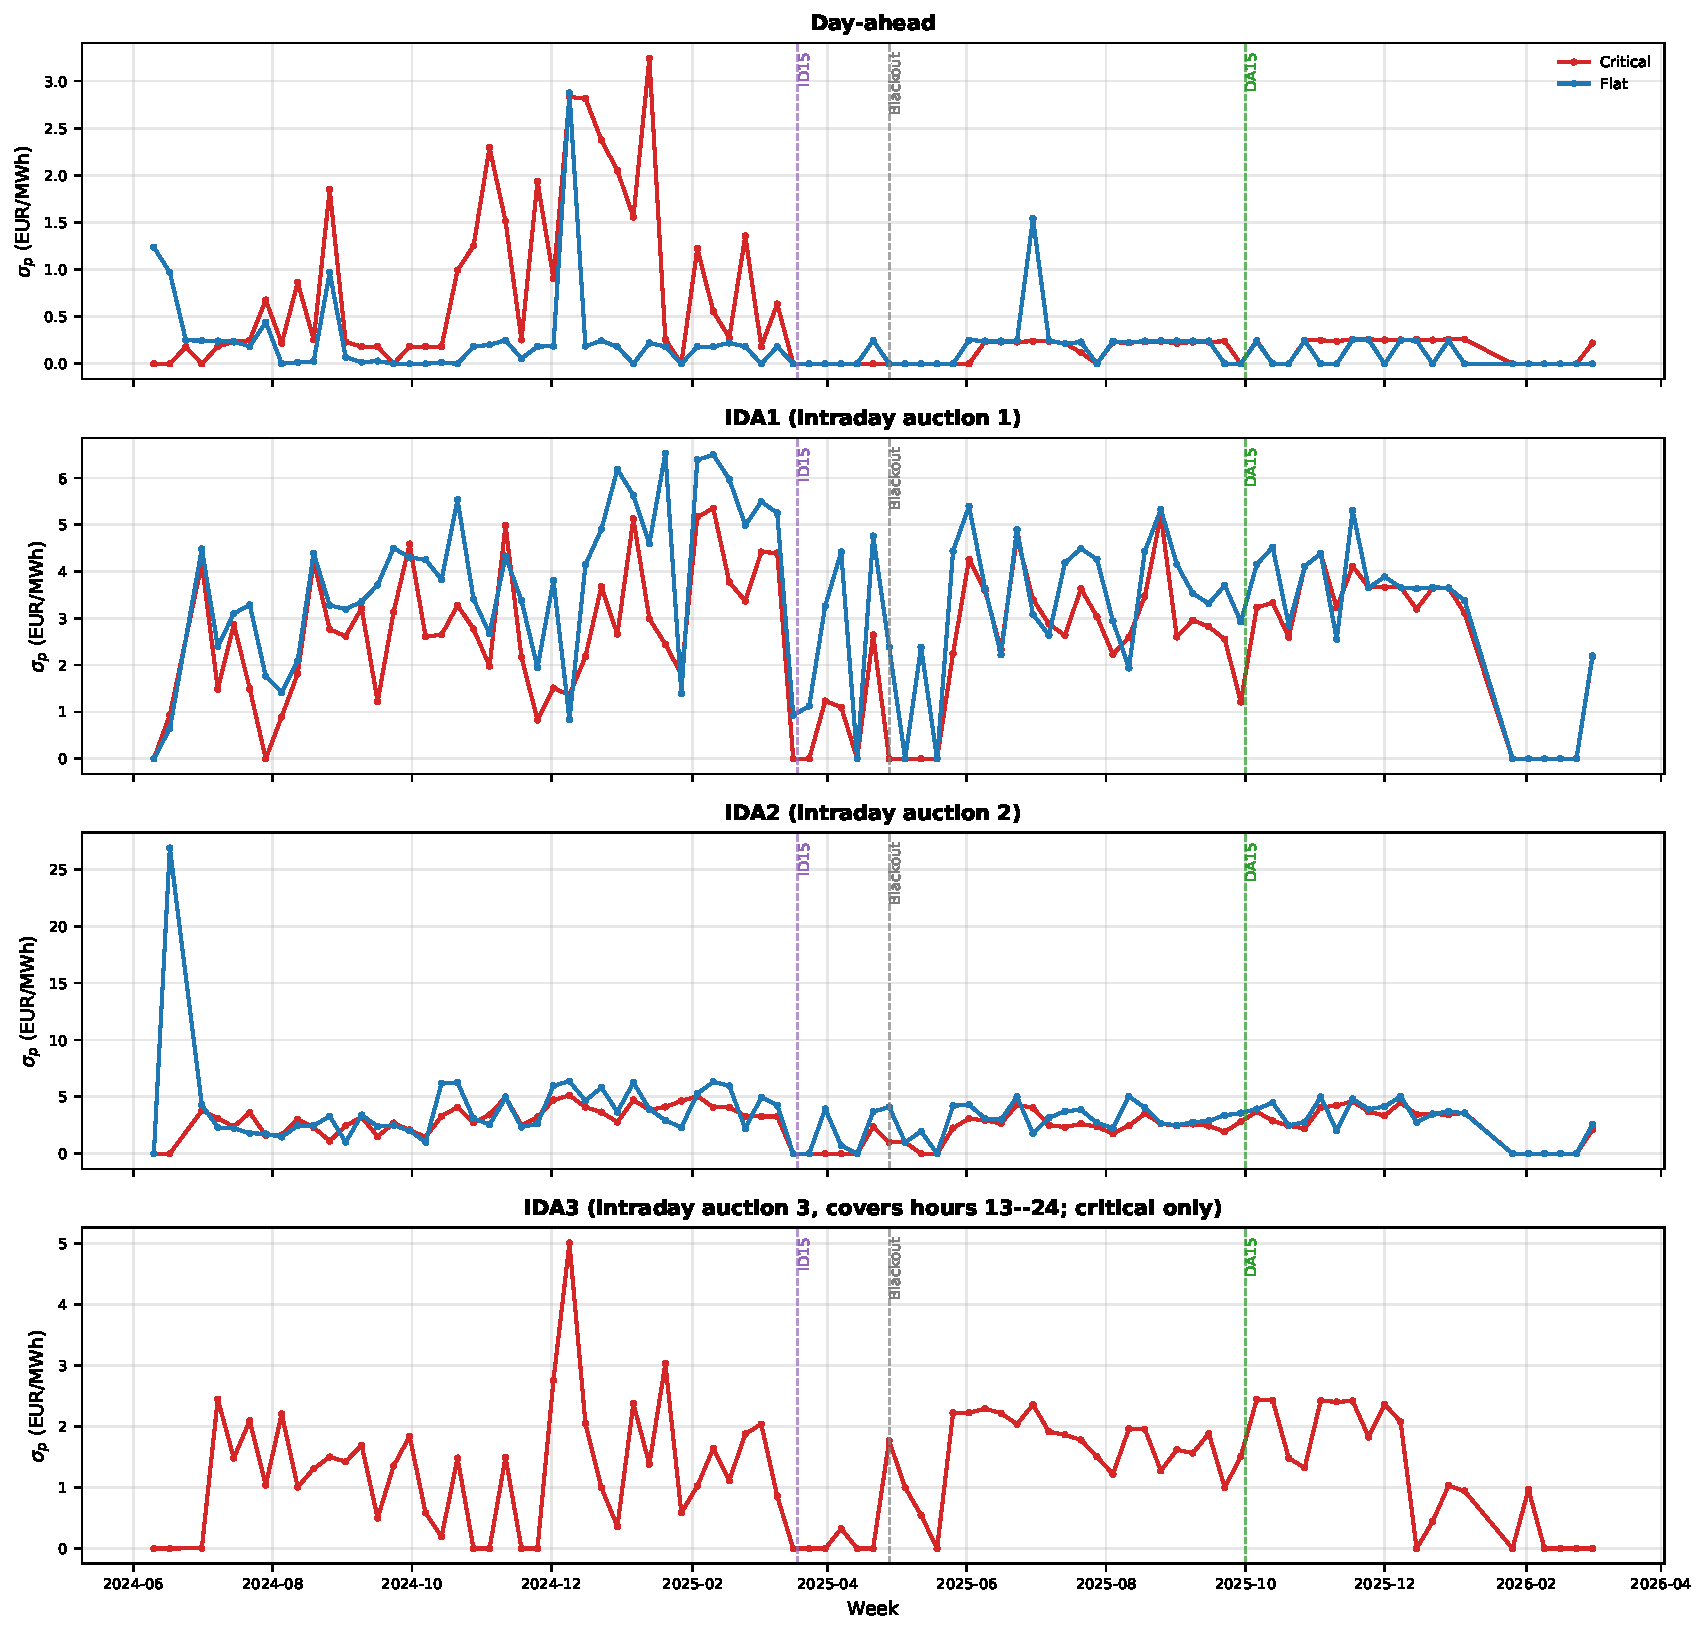
\includegraphics[width=\textwidth]{../../figures/thesis/fig_parallel_trends_sigma_p_per_session.pdf}
\caption{\textbf{Per-session parallel-trends diagnostic: weekly CCGT $\sigma_p$ by hour-class, 2024-06 to 2026-05.} Stacked panels: day-ahead, then each of the three IDA sessions. Red: critical hours (5--8, 16--22). Blue: flat hours (1--3). IDA3 covers only hours 13--24, so its panel reports critical only. Bandwidth $|p_k - \text{MCP}| \le 50$~EUR/MWh. Vertical dashes mark ID15 (2025-03-19), blackout (2025-04-28), and DA15 (2025-10-01). The IDA2 panel carries the most-active CCGT bid-shape pre-MTU15-IDA, and the three IDA panels visibly converge in level post-reform --- the per-session story behind the pooled Spec~C DiD.}
\label{fig:parallel-trends-sigma-p-per-session}
\end{figure}

% =====================================================================
\subsection{Post-DA15 IDA activity rise and the Fase~I displacement channel}\label{sec:5-ida-activity-fase1}
% =====================================================================

I compute pre-DA15 vs post-DA15 IDA bidding activity per session (block orders excluded). CCGT supply MW/day in IDA3 falls $15\%$; demand-side MW/day rises $+15$/$+10$/$+29\%$ across IDA1/IDA2/IDA3. The reading is a Fase~I displacement channel: re-reforzada (\S\ref{sec:institutional}) shifts CCGT dispatch from real-time into pre-IDA Fase~I, leaving residual imbalance for the demand side to absorb in late IDAs.

\begin{center}
\footnotesize
\setlength{\tabcolsep}{5pt}
\begin{tabular}{l c c c c c c c c}
\toprule
            & \multicolumn{2}{c}{\textbf{IDA1}} & \multicolumn{2}{c}{\textbf{IDA2}} & \multicolumn{2}{c}{\textbf{IDA3}} \\
\cmidrule(lr){2-3} \cmidrule(lr){4-5} \cmidrule(lr){6-7}
\textbf{Side / outcome}        & MW/day & tranches/curve & MW/day & tranches/curve & MW/day & tranches/curve \\
\midrule
CCGT supply        & $+11.6\%$ & $-3.8\%$ & $+0.5\%$ & $-1.9\%$ & $\mathbf{-15.0\%}$ & $-18.3\%$ \\
All supply         & $-5.7\%$  & $+16.7\%$ & $-10.2\%$ & $+6.9\%$ & $-17.9\%$ & $+3.8\%$ \\
Demand             & $\mathbf{+14.7\%}$ & $+14.9\%$ & $\mathbf{+10.0\%}$ & $+12.0\%$ & $\mathbf{+29.4\%}$ & $+9.7\%$ \\
\bottomrule
\end{tabular}
\captionof{table}{\textbf{IDA bidding activity, post-DA15 vs.\ pre-DA15 (reforzada-constant window).} Pre-DA15: 2025-04-28 to 2025-09-30 (post-blackout, post-ID15, pre-DA15); post-DA15: 2025-10-01 to 2025-12-31. ``MW/day'' is the sum of in-band offered quantities per session-day; ``tranches/curve'' is the mean over (date, unit, period) curves. Block orders excluded. CCGT IDA3 supply MW/day falls $15\%$ while demand-side IDA3 MW/day rises $29\%$ --- consistent with re-reforzada Fase~I displacement: CCGT is dispatched ahead of IDA close via Fase~I, leaving residual imbalance for the demand side to absorb in late IDAs.}
\label{tab:ida-activity-fase1}
\end{center}

Composes with the BSTS reading of Table~\ref{tab:bsts-ajuste-costs}: the TR-up shrink across the MTU15-DA cutover is procurement-timing substitution into pre-IDA Fase~I, not a market-mechanism cleanup. Industry source verbatim confirms (\S\ref{sec:results:granularity-vs-reforzada}).

% =====================================================================
\section{Continuous-market response at the three structural reforms}\label{app:continuous}
\phantomsection\label{sec:5-demand-buy-share}\phantomsection\label{tab:demand-buy-share}
% =====================================================================

BSTS on ES-leg continuous-market series under headline Spec~A. ID15 is the only structural cutover of the three: trade count jumps $+24{,}269$/day placebo-net ($p<0.001$) as participants take up the four 15-min contracts per clock-hour, and energy turnover drops $-12.36$ GWh/day placebo-net ($p<0.001$) as smaller contracts and partial migration toward the now-finer IDA auctions thin total volume. The continuous-market volume-weighted price is not separately identifiable from the renewable-driven price drop once year-interactions control the wind/solar coefficient (real $-43.6^{*}$, placebo-net $-18.3$ ns). ISP15 is a methodological null (settlement-only reform, contract grid unchanged); DA15 leaves the continuous-market contract grid alone (already 15-min post-ID15) and no outcome survives the year-interaction control. The continuous-market reading is consistent with the auction-side reading: granularity reforms shift the contract grid and the participation pattern, but the price-level component cannot be separated from the renewable-coefficient drift.

% =====================================================================
\section{Market-structure context}\label{app:context}
% =====================================================================

\subsection{The two-tier CCGT bid curve and the day-ahead/intraday contrast}
Every Big-4 CCGT fleet runs a two-tier day-ahead offer: a low \emph{competing} tier near marginal cost and a high \emph{parked} tier above the clearing-price ceiling. Withholding is firm-wide, not a Naturgy story. The same fleets bid a single competitive tier with negligible withholding in the intraday auction, after Fase~I has cleared. A unit's marginal cost does not change between two auctions hours apart. The parked tier is a placeholder rather than a Fase~I bid: Fase~I up-redispatch is settled through a separate restriction offer submitted to REE.\footnote{Procedure PO 3.2, settlement PO 14.4 ap.~20.1; see also \citet{boe_a_2025_5342,boe_a_2025_13076}.} MTU15-DA grants CCGT a within-hour degree of freedom over its competing tier; the CCGT auction-cleared scale-up in \S\ref{sec:results:6-4} is the competing tier expanding into the four quarters of each peak hour.

\subsection{Market concentration migrated from wholesale to ancillary services}
Wholesale-market HHI hovers around 1\,100 over 2016--2024 (below the moderate-concentration threshold of 1\,500) and falls mid-day when solar peaks (solar is less concentrated than the Big-3). Day-ahead restrictions upward HHI above 4\,000; deviations upward above 6\,000; tertiary upward around 5\,000. Median of 4 firms with accepted upward restrictions bids. As renewables eroded wholesale-market power, technical and locational requirements concentrated the ancillary markets that absorb their variability.

\subsection{The reforzada cost increase concentrates on CCGT}
The post-blackout REE intervention is technology-specific. \emph{Fase~I} (\emph{Resoluci\'on de restricciones t\'ecnicas por garant\'\i a de suministro}) is the pre-IDA technical-restrictions process REE runs on the PDBF programme: REE buys up-redispatch and sells down-redispatch to clear transmission-security constraints, settled pay-as-bid of a \emph{separate restriction offer} the unit submits to REE (Procedimiento de Operaci\'on PO~3.2; settlement PO~14.4 ap.~20.1). The Fase~I restriction offer is a distinct instrument from the unit's day-ahead market offer. \emph{Fase~II} (\emph{Resoluci\'on de restricciones por balance}) is the post-Fase-I rebalance that absorbs the up-redispatch back into the schedule through symmetric down-redispatch elsewhere (PO~3.2 §6); it has been operationally near-zero since 2024. Decomposing weekly dispatch into its components --- the day-ahead-cleared base (PDBC), bilateral executions, and the post-DA top-up routed through IDA and REE real-time redispatch --- the CCGT panel of Figure~\ref{fig:ree_intervention_by_tech} shows the day-ahead-cleared layer (blue) collapsing post-blackout while the IDA+REE-RT layer (red) balloons. Other technologies are largely flat across the same window.

\begin{figure}[h]
\centering
\includegraphics[width=\textwidth]{../../figures/working/fig_q_components_by_tech_weekly.pdf}
\caption{\textbf{Weekly three-component decomposition of dispatch, by technology.} PDBC (blue, day-ahead-cleared) $+$ bilateral executions (PDBF $-$ PDBC, green) $+$ post-DA REE intervention layer (PHF $-$ PDBF, red) $=$ final post-IDA dispatch (black, equivalent to PHF). The red layer aggregates everything that happens to the schedule between the day-ahead programme (PDBF) and the post-IDA programme (PHF): \emph{Fase~I} pre-IDA up-redispatch and \emph{Fase~II} rebalance under PO~3.2 (paid pay-as-bid via the restriction-offer channel of PO~14.4 ap.~20.1, distinct from the day-ahead market offer), plus the net of all IDA clearings and REE's post-IDA real-time technical-restrictions step. Within the red layer, Fase~I dominates the post-blackout growth (Figure~\ref{fig:efficiency_gains} and \S\ref{sec:results:granularity-vs-reforzada}). Vertical guides: MTU15-IDA, April 2025 blackout, MTU15-DA.}
\label{fig:ree_intervention_by_tech}
\end{figure}

This per-technology pattern is the cleanest evidence that the reforzada cost increase is a separate policy effect from the granularity reforms: a granularity reform that touched all bid-side firms equally would not produce a CCGT-only intervention pattern. The day-ahead CCGT cleared scale-up of \S\ref{sec:results:6-4} (DA15 only, critical hours) sits alongside this REE-intervention story: both are CCGT-side responses to the operational environment, but the granularity-driven response is competitive-clearing (and consumer-favourable) while the reforzada-driven response is REE-paid redispatch.

\subsection{Representative bid curves by technology}\label{app:context-bid-curves}
Figures~\ref{fig:bid-curves-by-tech}--\ref{fig:bid-curves-by-tech-flat} show real day-ahead bid step functions for one representative unit per technology, at an evening-ramp critical-hour quarter (Figure~\ref{fig:bid-curves-by-tech}) and at a flat overnight hour on a windy night (Figure~\ref{fig:bid-curves-by-tech-flat}). The visual contrast supports the \S\ref{sec:empirical:specC} exclusion of solar from Spec~C and the \S\ref{sec:results:6-5} reading of wind's small bid-shape DiD coefficients: dispatchables structure their competing tier inside the in-band region; renewables submit single or near-single blocks far below the band, so a within-band $\sigma_p$ or $\text{HHI}_p$ outcome is mechanically zero or one. Wind aggregators do occasionally submit multi-tranche micro-ladders below the band --- the WMVD088 panel in Figure~\ref{fig:bid-curves-by-tech-flat} shows 15 tranches over the narrow $[-20, +1.5]$~EUR/MWh range, consistent with the operational (imbalance-bill) rather than strategic incentive that drives wind's bidding (\S\ref{sec:results:6-5}) --- but these micro-ladders sit outside the in-band region and so do not enter the Spec~C outcomes.

\begin{figure}[H]
\centering
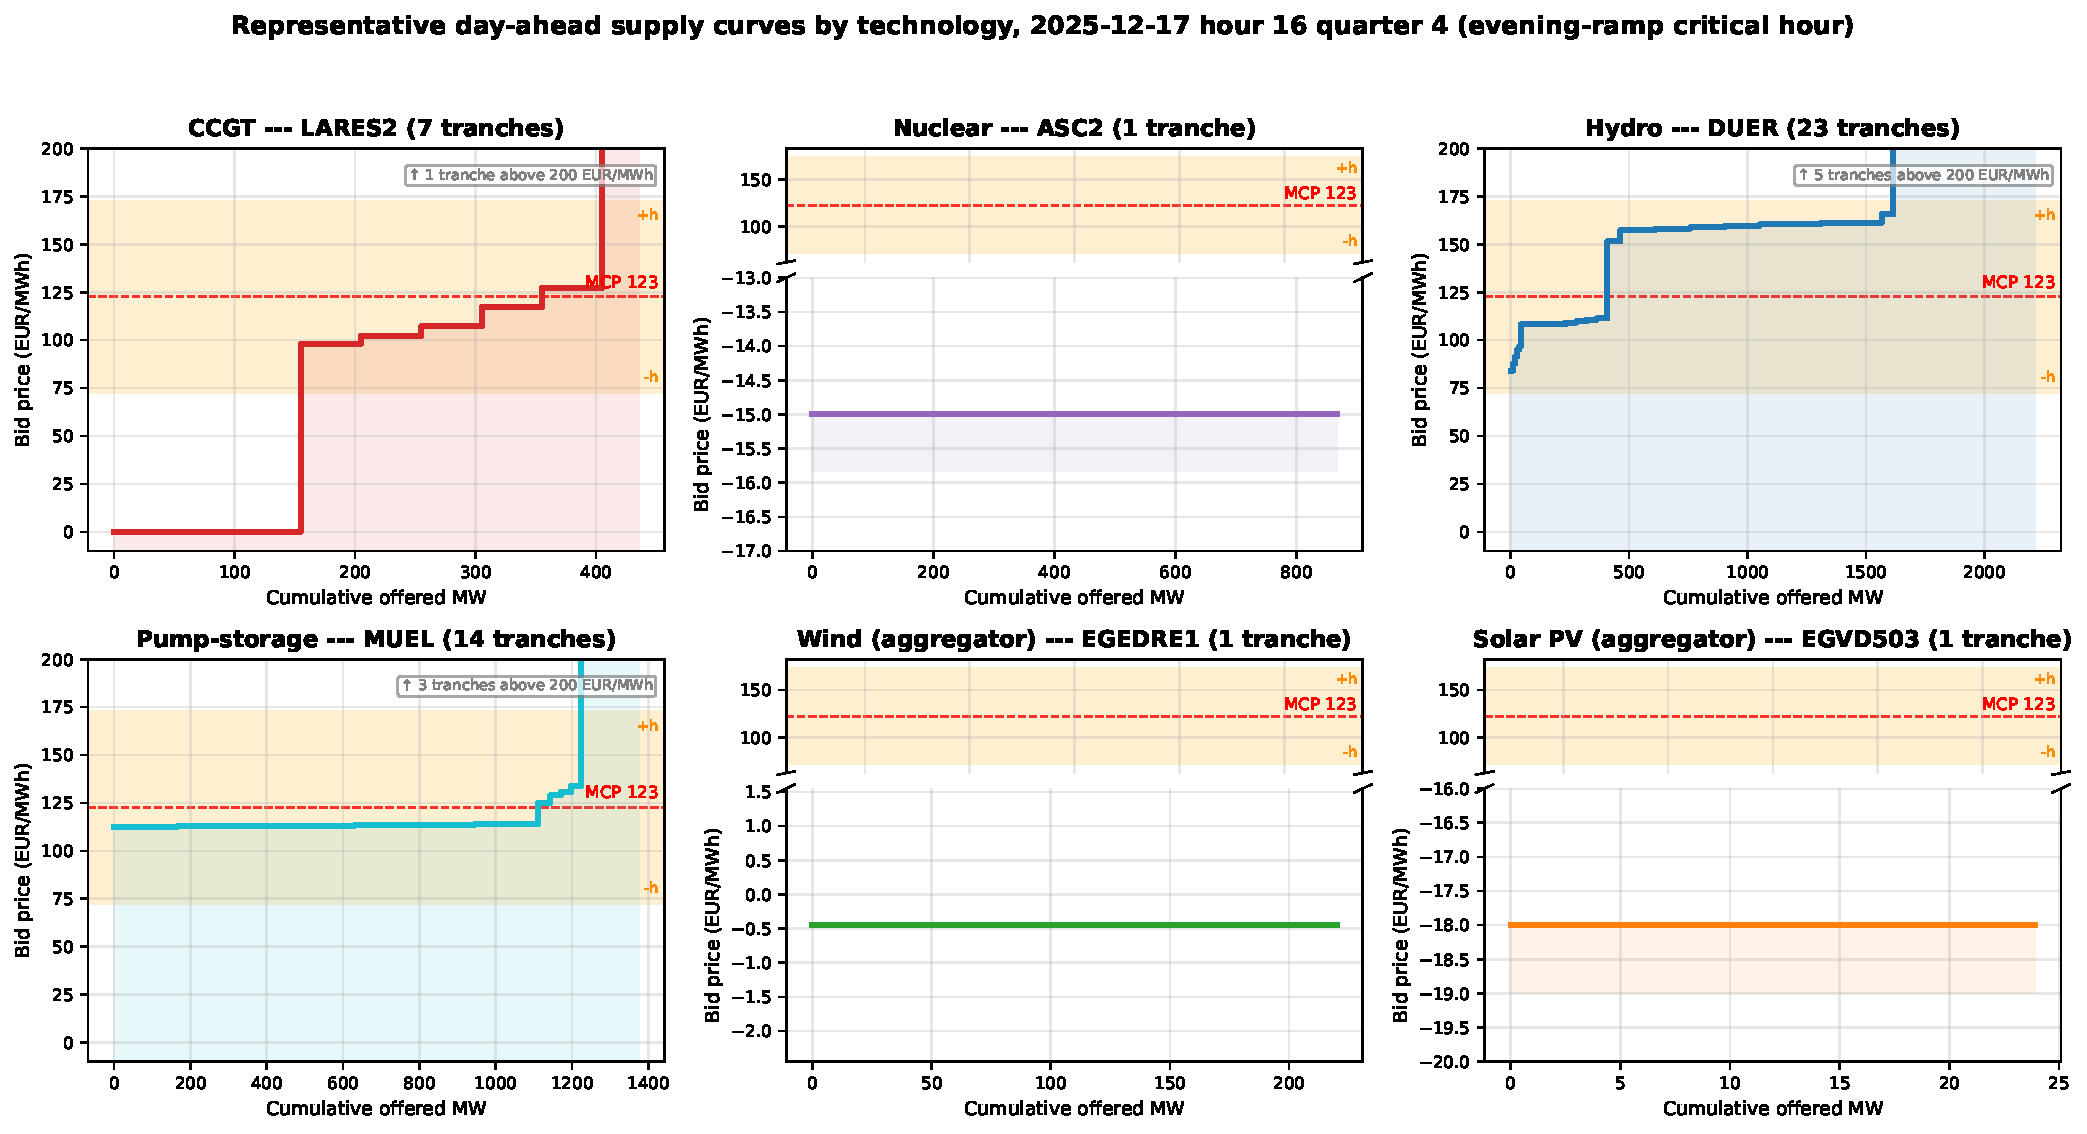
\includegraphics[width=\textwidth]{fig_bid_curves_by_tech.pdf}
\caption{\textbf{Representative day-ahead supply curves by technology}, 2025-12-17 hour 17 quarter 4 (post-MTU15-DA, evening-ramp critical hour). Red dashed: MCP; orange band: in-band region $[\text{MCP} \pm \delta]$ with $\delta=50$ (\S\ref{sec:data:bandwidth}). Panels with bid ranges far below the band use a broken y-axis for readability.}
\label{fig:bid-curves-by-tech}
\end{figure}

\begin{figure}[H]
\centering
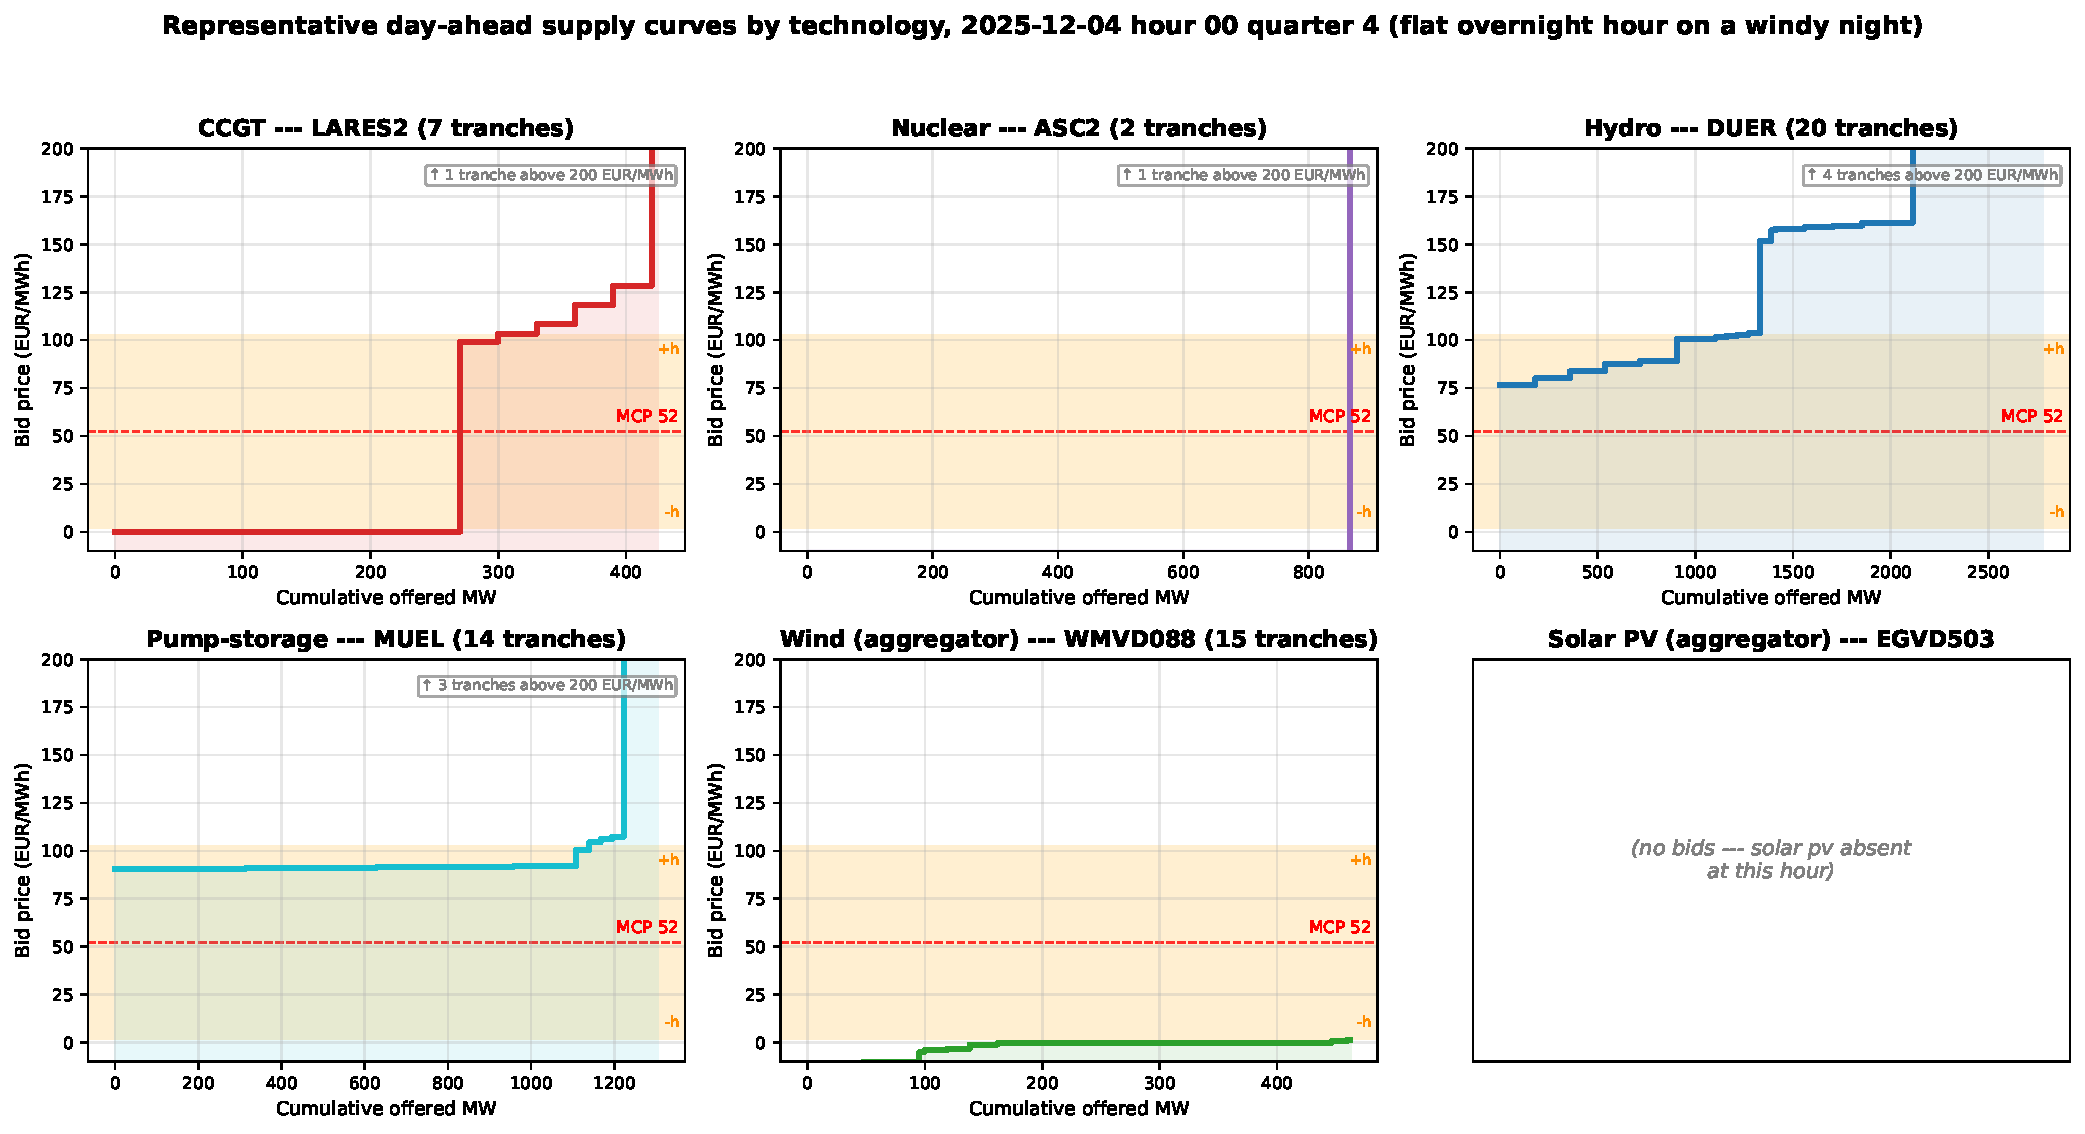
\includegraphics[width=\textwidth]{fig_bid_curves_by_tech_flat.pdf}
\caption{\textbf{Representative day-ahead supply curves by technology}, 2025-12-04 hour 01 quarter 4 (flat overnight hour on a windy night). Same colour scheme and broken y-axis convention as Figure~\ref{fig:bid-curves-by-tech}. The wind panel (WMVD088) shows a 15-tranche aggregator micro-ladder concentrated in $[-20, +1.5]$~EUR/MWh, well below the band.}
\label{fig:bid-curves-by-tech-flat}
\end{figure}

\paragraph{Buy vs sell IDA bid shapes (pre-ID15).} Figure~\ref{fig:buy-vs-sell-curves} shows representative IDA bid curves with the sell side (blue, ascending) and the buy side (red, descending) overlaid for one unit per tech in the pre-ID15 window, when buy-side activity was largest (\S\ref{sec:results:6-6b}). The shapes differ sharply across techs: CCGT and pump-storage submit dense sell ladders with a thin one-tranche buy book (sellers with a small rebuy option); hydro and renewable aggregators write multi-tranche curves on \emph{both} sides (forecast-driven rebalancing that can clear in either direction); nuclear barely participates on the buy side (the entire 9-month pre-ID15 window contains a single nuclear (date, session, period) cell with both sides). The renewable-aggregator panels are the clearest illustration of the buy-side rebalancing role of IDA: the buy and sell curves intersect near the realised MCP, and the aggregator clears on whichever side its quarter-level forecast falls.

\begin{figure}[H]
\centering
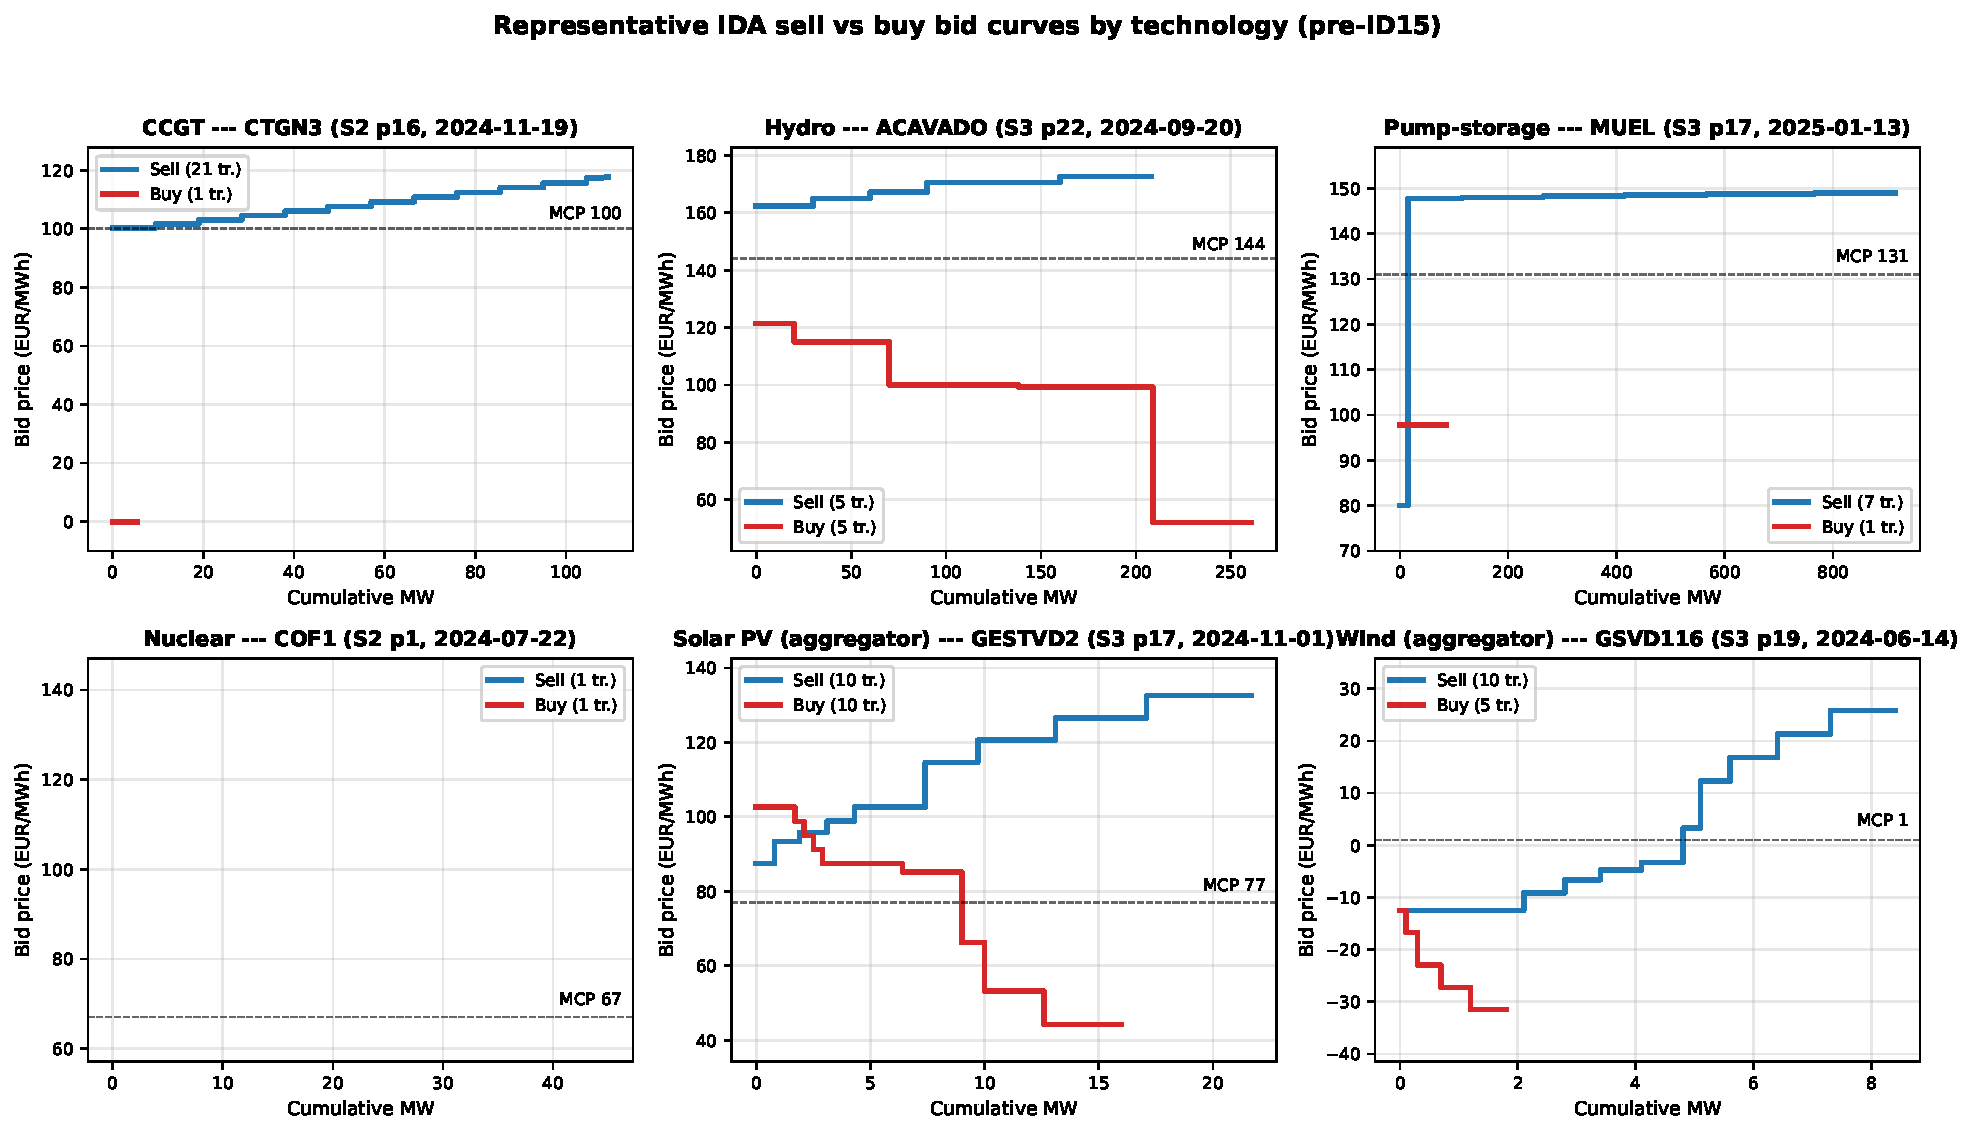
\includegraphics[width=\textwidth]{fig_buy_vs_sell_curves.pdf}
\caption{\textbf{Representative IDA sell vs buy bid curves by technology, pre-ID15.} One representative (unit, date, session, period) per tech. Blue: sell curve (supply, ascending in price). Red: buy curve (demand, descending in price). Dashed: MCP. Pre-ID15 window 2024-06-14 to 2025-03-18.}
\label{fig:buy-vs-sell-curves}
\end{figure}

% =====================================================================
\section{Theoretical derivations}\label{app:derivations}
% =====================================================================

\subsection{Setup details and information arrival}\label{app:setup}

This subsection records the timing of information arrival, the \citeauthor{ito_reguant_2016} residual-demand specification used throughout, and how that specification specialises when one or both markets are hourly.

\paragraph{Timing.} Stage~1 (DA): only $\bar A$ and the distribution of $\mu_t$ are known to the strategic bidder; the aggregator knows $\bar Y_h$, $\{\bar y_t\}$ and the distribution of $\eta_t$. Stage~2 (ID): $\mu_t$ has realised and is common knowledge to first order. Stage~3 (balancing): $\eta_t$ realises and settlement occurs at the balancing reference.

\paragraph{Residual demand (\citet{ito_reguant_2016} form).} The strategic residual monopolist with constant marginal cost $c$ serves what the operational aggregator does not cover, net of any arbitrage position $s_t$ carried from forward to spot. Per delivery product, with all quantities in MWh:
\begin{equation}
q_{1t} \;=\; \bar A_t \;-\; b_{1t}\, p_{1t} \;-\; s_t \;-\; S^{op}_{1t},
\qquad
q_{2t} \;=\; b_{2t}\,(p_{1t} - p_{2t}) \;+\; s_t \;-\; S^{op}_{2t},
\label{eq:rd}
\end{equation}
where $\bar A_t = \bar A + \mu_t$ is the per-subperiod demand intercept, $S^{op}_{mt}$ is the aggregator's offered MWh in market $m \in \{1, 2\}$ at subperiod $t$ (uniform $S^{op}_m / Q$ when market $m$ is hourly), and $b_{mt}$ is market thinness (with per-subperiod asymmetry allowed). We use $p_{mt}$ throughout for the per-subperiod price; when market $m$ is hourly, $p_{mt} \equiv p_m$ is constant in $t$ (the auction clears one price for the whole hour). The within-hour demand shock satisfies $\mathbb{E}[\mu_t] = 0$ and $\mathrm{Var}(\mu_t) = \sigma_\mu^2$; the aggregator's per-subperiod realisation is $y_t = \bar y_t + \eta_t$ with forecast-error variance $\sigma_\eta^2$.

\paragraph{Hourly residual demand by specialisation.} When market $m$ is hourly the bidder commits to the auction at one price for the hour, against the \emph{ex-ante expected} hourly aggregate of residual demand. The general per-subperiod object \eqref{eq:rd} specialises by setting $\bar A_t \equiv \bar A$ (the auction-time information set: $\mathbb{E}[(1/Q)\sum_t \mu_t] = 0$), $b_{mt} \equiv b_m$, $p_{mt} \equiv p_m$, and $S^{op}_{mt} \equiv S^{op}_m / Q$. The realised within-hour variation in $\mu_t$ that this substitution suppresses does not vanish from the model: it loads onto the balancing residual (\S\ref{app:balancing}) and shows up in the system imbalance cost $C^I_{\text{sys}}$ in the welfare derivations (\S\ref{app:welfare}). In $(1,1)$ both equations reduce to one product apiece; in $(1,Q)$ only the spot demand keeps the per-period index.

The two-stage analysis here covers the forward-spot auction pair. The balancing market enters only as the ex-post settlement reference; we collapse it into the balancing discrepancy $\Delta_t$ used in \S\ref{app:balancing}.

\subsection{Operational aggregator: closed-form gain from per-period scheduling}\label{app:aggregator}

We derive the aggregator's expected hedging gain $G(\Delta_\eta)$ from per-period (rather than hourly) spot scheduling in closed form under uniform shocks. We then explain why the aggregator's \emph{individual} forward-vs-spot allocation is not pinned down by an interior first-order condition under standard penalty specifications, and why the empirical migration onto the granular leg (Result 3) is therefore an equilibrium statement about $G$ being positive, not an aggregator-level $\Delta^*$ identification.

\subsubsection{Problem statement and primitives}\label{app:aggregator:problem}
The aggregator allocates total hourly expected production $\bar Y_h$ between forward and spot. Forecast-error shock $\eta_t \sim \mathrm{Uniform}[-\Delta_\eta, \Delta_\eta]$, i.i.d.\ across $t$, with variance $\sigma_\eta^2 = \Delta_\eta^2/3$. We set the structural per-subperiod expected production constant ($\bar y_t = \bar Y_h/Q$) for the closed-form derivation; the structural variation $\sigma_a^2 = \mathrm{Var}(\bar y_t - \bar Y_h/Q)$ adds linearly to $G$ and is handled in the closing remark. Imbalance penalty is $\gamma|\mathcal{I}_t|$ per period (linear in the magnitude of the gap).

\subsubsection{Expected penalty under each regime}\label{app:aggregator:gain}
\paragraph{Granular spot $(Q^S = Q)$.} At Stage~2 the aggregator observes $\eta_t$ and sets the per-subperiod allocation $S_{2t}^{op}{}^* = \bar y_t + \eta_t - S_1^{op}/Q$. The realised per-period imbalance is $0$ (modulo post-Stage-$2$ noise $\varepsilon_t$, which is regime-invariant and we drop for clarity):
\[
\mathbb{E}[\mathcal{C}_{\text{gran}}] \;=\; 0.
\]

\paragraph{Hourly spot $(Q^S = 1)$.} The aggregator commits $S_1^{op} + S_2^{op} = \bar Y_h$ before $\eta_t$ resolves; the per-subperiod schedule is therefore uniform at $\bar Y_h/Q$. With $\bar y_t = \bar Y_h/Q$ the per-period imbalance is exactly $\eta_t$. For $\eta_t \sim \mathrm{Uniform}[-\Delta_\eta, \Delta_\eta]$:
\[
\mathbb{E}|\eta_t| \;=\; \dfrac{\Delta_\eta}{2}, \qquad \mathbb{E}[\mathcal{C}_{\text{hour}}] \;=\; \gamma Q \cdot \dfrac{\Delta_\eta}{2}.
\]

\paragraph{Closed-form hedging gain.} The aggregator's expected hourly saving from per-period (granular) spot scheduling relative to hourly spot scheduling is
\begin{equation}
\boxed{\;G(\Delta_\eta) \;=\; \mathbb{E}[\mathcal{C}_{\text{hour}}] - \mathbb{E}[\mathcal{C}_{\text{gran}}] \;=\; \dfrac{\gamma Q \, \Delta_\eta}{2}.\;}
\label{eq:agg-gain}
\end{equation}
Comparative statics are immediate:
\begin{equation}
\dfrac{\partial G}{\partial \Delta_\eta} \;=\; \dfrac{\gamma Q}{2} \;>\; 0, \qquad \dfrac{\partial G}{\partial \sigma_\eta^2} \;=\; \dfrac{\gamma Q}{2\sqrt{3}\,\sigma_\eta} \;>\; 0.
\label{eq:agg-cs}
\end{equation}
The gain is strictly positive and strictly increasing in the forecast-error variance. The structural-variation extension is additive: adding $\sigma_a^2$ contributes $\gamma Q \, \sigma_a$ (under the same uniform-shock convention applied to the structural component), which preserves \eqref{eq:agg-cs} and the sign of the gain.

\subsubsection{Why $\Delta^*$ is not pinned down by an individual FOC}\label{app:aggregator:shift}
A natural follow-up is to ask whether $G$ pins down the aggregator's allocation $S_1^{op}$ via a first-order condition. It does not. The aggregator's expected profit under either regime is
\[
\Pi(S_1^{op}) \;=\; (p_1 - p_2)\, S_1^{op} \;+\; p_2 \, \bar Y_h \;-\; \mathbb{E}[\mathcal{C}],
\]
where the expected imbalance cost $\mathbb{E}[\mathcal{C}]$ is independent of $S_1^{op}$ once we impose the no-average-bias condition $S_1^{op} + S_2^{op} = \bar Y_h$. The FOC reduces to $p_1 - p_2 = 0$, a corner solution rather than an interior $\Delta^*$. This is a structural feature of the price-taker setup: the imbalance cost depends on the resolution of information (whether the aggregator can react to $\eta_t$), not on how forward and spot allocations split.

The migration onto the granular leg is therefore an \emph{equilibrium} statement: across aggregators, $G(\Delta_\eta) > 0$ generates a positive premium for participation on the granular spot; equilibrium prices adjust so that the wedge $p_1 - p_2$ partially incorporates this premium; and the empirical aggregate shift in supply onto the granular leg (Result~3, sell-share rise of nuclear and wind at the March reform) is the equilibrium counterpart. We claim only the direction of the shift via $G > 0$; we do not derive a level prediction for $\Delta^*$ at the individual aggregator's optimum.

\subsection{Strategic bidder: optimal two-tranche ladder}\label{app:tranche}

We derive the strategic bidder's closed-form two-tranche ladder under uniform-price clearing, the FOCs in $(p^L, p^H, k^L)$, the equilibrium spread $\Delta p^* = \Delta_\mu/(2 b)$, and a stylisation note that flags the simplification absorbed into the boundary condition.

\subsubsection{Profit under uniform-price clearing}\label{app:tranche:profit}
The strategic bidder is the residual monopolist; there is no higher-priced fringe bid above its top tranche. Under uniform-price clearing (as in OMIE day-ahead and intraday auctions), the clearing price is therefore set by the marginal accepted tranche of the strategic bidder's own ladder: $p^L$ when only the low tranche clears, $p^H$ when both clear. For a delivery product at which the residual-demand intercept is $\bar A + \mu$ (with $\mu \sim \mathrm{Uniform}[-\Delta_\mu, +\Delta_\mu]$), the strategic bidder commits a ladder $\{(p^L, k^L), (p^H, k^H)\}$ with $p^L \le p^H$, $k^L + k^H = K$ \emph{before} $\mu$ realises. We use $b$ for the market thinness ($b_{1t}$ or $b_{2t}$, depending on which market the ladder is on).

\emph{Crossover demand state $\mu^*$.} Residual demand at price $p^L$ in demand state $\mu$ is $\bar A + \mu - b\, p^L$. The cutoff $\mu^*$ is the demand state at which this residual demand exactly equals the low-tranche volume:
\[
\bar A + \mu^* - b\, p^L \;=\; k^L \qquad \Longleftrightarrow \qquad \mu^* \;\equiv\; k^L + b\, p^L - \bar A.
\]
For $\mu \le \mu^*$ residual demand at $p^L$ is at most $k^L$, so only the low tranche clears and the auction prices at $p^L$. For $\mu > \mu^*$ residual demand exceeds $k^L$ at $p^L$, so both tranches clear and uniform pricing carries $p^H$ on the full capacity $K$. The cleared MWh at $\mu$ is then
\[
q(\mu) = \begin{cases} q^L \;=\; k^L & \text{if } \mu \le \mu^*, \\ K \;=\; k^L + k^H & \text{if } \mu > \mu^*. \end{cases}
\]
The two-tranche reduction treats $q^L = k^L$ as constant on $\mu \in [-\Delta_\mu, \mu^*]$ rather than tracking the smooth residual-demand schedule below $\mu^*$; this is the stylisation absorbed into the boundary condition (see closing note of this subsection). Expected profit per delivery product is
\begin{equation}
\mathbb{E}[\pi]
\;=\; \frac{1}{2\Delta_\mu}\!\left[\int_{-\Delta_\mu}^{\mu^*}\!(p^L - c)\,q^L\,d\mu \;+\; \int_{\mu^*}^{\Delta_\mu}\!(p^H - c)\,K\,d\mu\right],
\label{eq:Epi-uniform}
\end{equation}
with $(p^H - c)\,K$ in the second integrand reflecting that all $K$ units fetch $p^H$ when the high tranche is marginal.

\emph{Implicit price cap via the demand support.} Real auctions impose an explicit price cap $p^{\max}$ (around EUR\,3000/MWh in MIBEL); the formulation above absorbs the cap into the demand support, since the bidder pushes $p^H$ to the price that clears $K$ at the highest demand realisation $\mu = \Delta_\mu$ (see FOC below). The two parameterisations are equivalent up to a constant rescaling and we keep $\Delta_\mu$ for tractability.

\subsubsection{First-order conditions}\label{app:tranche:foc}
Take derivatives in $(p^L, p^H, k^L)$ holding $K = k^L + k^H$ fixed. Define $w^L = k^L/K$, $w^H = k^H/K$.

\paragraph{FOC in $p^H$.}
\[
\frac{\partial \mathbb{E}[\pi]}{\partial p^H} \;=\; \frac{1}{2 \Delta_\mu} \int_{\mu^*}^{\Delta_\mu} K\, d\mu \;=\; \frac{K(\Delta_\mu - \mu^*)}{2\Delta_\mu} \;>\; 0
\]
unless $\mu^* = \Delta_\mu$. The derivative is strictly positive at any interior $\mu^*$: raising $p^H$ earns extra mark-up on the full capacity $K$ in every demand state above $\mu^*$, and (within the interior) carries no quantity loss because both tranches still clear. The bidder therefore pushes $p^H$ to the boundary where even the highest demand state $\mu = \Delta_\mu$ just clears full capacity: residual demand at $p^H$ equals $K$ when $\bar A + \Delta_\mu - b\, p^H = K$, i.e.\
\[
p^{H} \;=\; (\bar A + \Delta_\mu - K)/b \quad\text{at the binding boundary.}
\]
Substituting the symmetric-solution value $\mu^* = 0$ (derived below from the joint FOCs) gives the closed form $p^{H*} = (\bar A + b c)/(2 b) + \Delta_\mu/(4 b)$.

\paragraph{FOC in $p^L$.}
\[
\frac{\partial \mathbb{E}[\pi]}{\partial p^L} \;=\; \frac{1}{2\Delta_\mu}\!\left[\int_{-\Delta_\mu}^{\mu^*}\!q^L \, d\mu \;+\; (p^L - c) q^L \cdot \frac{\partial \mu^*}{\partial p^L}\right] \;=\; \frac{1}{2\Delta_\mu}\!\left[(\mu^* + \Delta_\mu)\, q^L \;+\; (p^L - c) q^L\, b\right] \;=\; 0.
\]
Solving: $\mu^* + \Delta_\mu + b(p^L - c) = 0$, i.e.\ $\mu^* = -\Delta_\mu - b(p^L - c)$. Combined with the definition $\mu^* = k^L + b p^L - \bar A$, this gives $k^L = \bar A - b p^L + \mu^*$. At $\mu^* = 0$: $p^{L*} = (\bar A + b c)/(2 b) - \Delta_\mu/(4 b)$.

\paragraph{FOC in $k^L$.} Differentiating \eqref{eq:Epi-uniform} in $k^L$ with $K = k^L + k^H$ held fixed ($\partial k^H/\partial k^L = -1$, $\partial K/\partial k^L = 0$), and using $\partial \mu^*/\partial k^L = 1$ from the definition of $\mu^*$:
\begin{align*}
\frac{\partial \mathbb{E}[\pi]}{\partial k^L} \;=\; & \underbrace{\frac{p^L - c}{2\Delta_\mu}\,(\mu^* + \Delta_\mu)}_{\text{direct: more MWh sold at } p^L \text{ in regime 1}} \\
& \;-\; \underbrace{\frac{p^H - c}{2\Delta_\mu}\,(\Delta_\mu - \mu^*)}_{\text{boundary: probability mass shifts from regime 2 to regime 1 as } \mu^* \uparrow} \;=\; 0.
\end{align*}
The two terms have opposite signs: enlarging the low tranche earns extra inframarginal markup over $[-\Delta_\mu, \mu^*]$, but shifts probability mass out of the high-markup regime $(p^H - c) > (p^L - c)$. The optimum balances them. At the symmetric solution $\mu^* = 0$, the FOC becomes $(p^L - c) = (p^H - c)$ scaled by the $1/2$ probability of each regime --- not the literal equation $p^L = p^H$, but rather $p^L$ and $p^H$ are chosen so that the marginal benefit of one extra low-tranche MWh exactly matches the marginal cost. With $p^{L*}$ and $p^{H*}$ pinned by their own FOCs, the joint solution requires $\mu^* = 0$ exactly: \textbf{$\mu^* = 0$ is the median demand cutoff} --- the bidder structures the ladder so that exactly half the demand realisations clear only the low tranche and half clear both. Substituting $\mu^* = 0$ in $k^L = \bar A - b p^{L*} + \mu^*$ and the closed form for $p^{L*}$,
\[
k^{L*} \;=\; \bar A - b\bigg(\frac{\bar A + bc}{2b} - \frac{\Delta_\mu}{4b}\bigg) \;=\; \frac{\bar A - b c}{2} + \frac{\Delta_\mu}{4}.
\]

\paragraph{Closed-form interior optimum.}
\begin{equation}
\boxed{\;p^{L*} = \frac{\bar A + b\, c}{2 b} - \frac{\Delta_\mu}{4 b},
\quad
p^{H*} = \frac{\bar A + b\, c}{2 b} + \frac{\Delta_\mu}{4 b},
\quad
\mu^{**} = 0,
\quad
k^{L*} = \frac{\bar A - b\, c}{2} + \frac{\Delta_\mu}{4}.\;}
\label{eq:tranche-spread}
\end{equation}

\paragraph{Comparative statics.} From \eqref{eq:tranche-spread}, the optimal pre-realisation tranche spread is
\begin{equation}
\Delta p^* \;=\; p^{H*} - p^{L*} \;=\; \frac{\Delta_\mu}{2 b}.
\label{eq:spread-cs}
\end{equation}
Running the same argument on the hourly aggregate $\tilde\mu = Q^{-1} \sum_t \mu_t$ (variance $\sigma_\mu^2/Q < \sigma_\mu^2$) gives a strictly smaller optimal spread, $\Delta p^*|_{\text{hourly}} = \tilde\Delta_\mu/(2 b)$ with $\tilde\Delta_\mu = \Delta_\mu/\sqrt{Q}$. The per-period ladder is therefore strictly richer than its hourly counterpart by a factor $\sqrt{Q}$.

\paragraph{Stylisation note.} The closed-form \eqref{eq:tranche-spread} requires that the capacity $K$ be tuned to the boundary condition $p^{H*}$ binds at the highest demand realisation $\mu = \Delta_\mu$; for general $K$ the FOC in $p^L$ also picks up a term $-bK(p^H-c)$ from the second integrand of \eqref{eq:Epi-uniform}, and the optimum shifts off the symmetric form. The closed form is therefore a stylised approximation, with the auction microfoundation absorbed into the boundary condition. Comparative statics in $\Delta_\mu$ and $b$ are robust to this stylisation: $\Delta p^*$ widens with the demand range and contracts with thinness.

Empirical measures of within-curve bid-shape dispersion (MW-weighted price SDs, effective tranche counts) are motivated by this widening but are not derived from the two-state reduction --- they require richer bid-curve structure than the two-tranche approximation supports.

\subsection{$(1,1)$ equilibrium}\label{app:state-60-60}

We solve the pre-reform game by backward induction: the Stage~2 best response (\S\ref{app:60-60:stage2}), then the four arbitrage regimes at Stage~1 (\S\ref{app:60-60:stage1}). The scarcity wedge $p_1 > p_2 > c$ survives in regimes (1), (3), and (4); only competitive full arbitrage closes it.

\subsubsection{Stage 2 best response}\label{app:60-60:stage2}
The strategic bidder's Stage~2 problem, taking $p_1$, $q_1$ and $s$ as given:
\[
\max_{p_2} (p_2 - c) q_2 \quad\text{s.t.}\quad q_2 = b_2(p_1 - p_2) + s - S^{op}_2.
\]
FOC: $b_2(p_1 - p_2) + s - S^{op}_2 + (p_2 - c)(-b_2) = 0$, giving
\begin{equation}
p_2^*(p_1, s) \;=\; \frac{p_1 + c}{2} + \frac{s - S^{op}_2}{2\, b_2}.
\label{eq:p2-60-60}
\end{equation}

\subsubsection{Stage 1 best response and equilibrium in $(p_1, s)$}\label{app:60-60:stage1}
Substituting \eqref{eq:p2-60-60} into the strategic bidder's total profit and using $q_1 = \bar A - b_1 p_1 - s - S^{op}_1$,
\[
\Pi(p_1, s) \;=\; (p_1 - c)(\bar A - b_1 p_1 - s - S^{op}_1) \;+\; (p_2^*(p_1, s) - c) q_2^*(p_1, s).
\]
The four arbitrage cases pin $s$ differently.

\paragraph{(R1) No arbitrage ($s = 0$).} The strategic bidder solves a Cournot problem in each market separately. The forward FOC gives $p_1^* = (\bar A - S^{op}_1 + b_1 c)/(2 b_1)$. Combining with \eqref{eq:p2-60-60} yields $p_1^* > p_2^* > c$ and $q_1, q_2 > 0$ (\citeauthor{ito_reguant_2016} Result~1).

\paragraph{(R2) Full arbitrage ($p_1 = p_2$).} Setting $p_1 = p_2$ in \eqref{eq:p2-60-60} gives $s = b_2(p_1 - c) + S^{op}_2$. Substituting back, total cleared MWh $q_1 + q_2 = \bar A - b_1 p_1 - S^{op}_1 - S^{op}_2 = \bar A - b_1 p_1 - \bar Y_h$ (using $S^{op}_1 + S^{op}_2 = \bar Y_h$). The strategic bidder maximises $(p_1 - c)(\bar A - b_1 p_1 - \bar Y_h)$, giving
\begin{equation}
p_1^{*,F} \;=\; \frac{\bar A - \bar Y_h + b_1 c}{2 b_1}, \qquad p_2^{*,F} \;=\; p_1^{*,F}.
\label{eq:p1-60-60-full}
\end{equation}
Note that $s > 0$ \emph{reduces} the strategic bidder's total output relative to no arbitrage (\citeauthor{ito_reguant_2016} Result~2): even competitive arbitrage does not restore competitive prices, because the bidder withholds more in response.

\paragraph{(R3) Limited arbitrage ($s \le K$ binding).} If $K$ is below the full-arbitrage level, $s = K$ binds and $p_1 - p_2 > 0$. From \eqref{eq:p2-60-60}, $p_1 - p_2 = (p_1 - c)/2 - (K - S^{op}_2)/(2 b_2)$; the wedge depends on $K$ and on $S^{op}_2$ (\citeauthor{ito_reguant_2016} Result~3). The smaller $K$, the larger the residual wedge.

\paragraph{(R4) Strategic arbitrage.} The arbitrageur maximises $\pi^A(s) = s(p_1 - p_2)$ subject to \eqref{eq:p2-60-60}:
\[
\pi^A(s) \;=\; s\!\left[\frac{p_1 - c}{2} - \frac{s - S^{op}_2}{2\, b_2}\right].
\]
FOC in $s$:
\[
\frac{p_1 - c}{2} - \frac{2 s - S^{op}_2}{2\, b_2} \;=\; 0
\quad\Longleftrightarrow\quad
s^{*,S}(p_1) \;=\; \frac{b_2 (p_1 - c)}{2} + \frac{S^{op}_2}{2}.
\]
Substituting into \eqref{eq:p2-60-60} (with $S^{op}_2 \to 0$ for clarity in the wedge derivation),
\begin{equation}
p_2^{*,S} \;=\; \frac{p_1 + c}{2} + \frac{b_2(p_1 - c)/2}{2\, b_2} \;=\; \frac{p_1 + c}{2} + \frac{p_1 - c}{4} \;=\; \frac{3 p_1 + c}{4}.
\label{eq:p2-strategic-derived}
\end{equation}
The forward-spot wedge is $p_1 - p_2^{*,S} = (p_1 - c)/4$, matching \eqref{eq:strategic-arb} in the main body (\citeauthor{ito_reguant_2016} Result~4). The Stage~1 forward price $p_1^{*,S}$ is the maximiser of the strategic bidder's compound profit; algebra in the standard quadratic gives $p_1^{*,S} - c = 8 (\bar A - b_1 c - \bar Y_h)/(16 b_1 - b_2)$ at $S^{op}_2 = 0$, $S^{op}_1 = \bar Y_h$. The wedge $(p_1^{*,S} - c)/4 > 0$ persists at the equilibrium price.

\subsection{$(1,Q)$ equilibrium}\label{app:state-60-15}

Forward hourly, spot per-period. We derive the per-product spot best response, work through full and strategic arbitrage to obtain the within-block dispersion equations, and finally compute the within-hour wedge SD in this asymmetric state.

The strategic bidder's Stage~2 problem now has $Q$ spot products. Directly from the spot residual demand $q_{2t} = b_{2t}(p_1 - p_{2t}) + s_t - S^{op}_{2t}$ in \eqref{eq:rd} and the FOC $q_{2t} = b_{2t}(p_{2t}-c)$, the strategic per-period spot best response is
\begin{equation}
p_{2t}^*(p_1, s_t) \;=\; \frac{p_1 + c}{2} \;+\; \frac{s_t - S^{op}_{2t}}{2\, b_{2t}}.
\label{eq:p2-60-15-foc}
\end{equation}
The cross-product variation in $p_{2t}^*$ in this state comes purely from per-subperiod variation in $b_{2t}$, $s_t$, $S^{op}_{2t}$ --- the forward price $p_1$ is hourly and shared, and $\mu_t$ does not enter the spot demand directly (it acts only through the forward-cleared volume, which is uniform per subperiod when forward is hourly).

\subsubsection{Full arbitrage: block parity and within-block dispersion}\label{app:60-15:full}
Block parity requires $p_1 = (1/Q) \sum_t p_{2t}$. Substituting \eqref{eq:p2-60-15-foc},
\[
p_1 \;=\; \frac{p_1 + c}{2} + \frac{1}{2 Q}\!\sum_t\!\frac{s_t - S^{op}_{2t}}{b_{2t}}
\quad\Longleftrightarrow\quad
p_1 - c \;=\; \frac{1}{Q}\!\sum_t\!\frac{s_t - S^{op}_{2t}}{b_{2t}}.
\]
Setting $S^{op}_{2t} \equiv 0$ and uniform arbitrage $s_t \equiv \bar s$ to isolate the thinness mechanism, and $Q = 2$ for concreteness,
\[
p_1 - c \;=\; \frac{\bar s}{2}\!\left(\frac{1}{b_{21}} + \frac{1}{b_{22}}\right) \;=\; \frac{\bar s}{2}\cdot\frac{b_{21}+b_{22}}{b_{21} b_{22}}
\quad\Longleftrightarrow\quad
\bar s \;=\; \frac{2(p_1 - c)\, b_{21} b_{22}}{b_{21} + b_{22}}.
\]
The within-block dispersion follows from differencing $p_{2t}^*$ across $t$:
\[
p_{21} - p_{22} \;=\; \bigg(\frac{\bar s}{2 b_{21}} - \frac{\bar s}{2 b_{22}}\bigg) \;=\; \frac{\bar s}{2}\cdot\frac{b_{22} - b_{21}}{b_{21}\, b_{22}}.
\]
Substituting $\bar s$ from above,
\begin{equation}
\boxed{\;p_{21} - p_{22} \;=\; (p_1 - c)\cdot \frac{b_{22} - b_{21}}{b_{21} + b_{22}}\;}\qquad\text{(full arbitrage)}.
\label{eq:within-block-full}
\end{equation}

\subsubsection{Strategic arbitrage: block wedge and attenuated dispersion}\label{app:60-15:strategic}
The strategic arbitrageur internalises price impact and stops at
\[
p_1 - (1/Q)\sum_t p_{2t} \;=\; \frac{p_1 - c}{4}.
\]
The block-wedge condition is the average of \eqref{eq:strategic-arb} across the $Q$ matched spot products. Repeating the algebra of \S\ref{app:60-15:full} with this modified parity, the arbitrage position $\bar s$ falls to exactly half of the full-arbitrage value:
\[
\bar s^{S} \;=\; \frac{(p_1 - c)\, b_{21} b_{22}}{b_{21} + b_{22}} \;=\; \frac{\bar s^{F}}{2}.
\]
The within-block dispersion correspondingly becomes
\begin{equation}
\boxed{\;p_{21} - p_{22} \;=\; \frac{p_1 - c}{2}\cdot\frac{b_{22} - b_{21}}{b_{21} + b_{22}}\;}\qquad\text{(strategic arbitrage)}.
\label{eq:within-block-strategic}
\end{equation}
The dispersion is attenuated by a factor of two relative to the full-arbitrage case, reflecting the smaller arbitrage volume traded under strategic incentives.

\subsubsection{Two-tranche ladder on the spot side}\label{app:60-15:ladder}
The strategic bidder posts per-product spot ladders. Applying \S\ref{app:tranche} with $b \to b_{2t}$ gives ladder spread $\Delta p^*_{2t} = \Delta_\mu/(2 b_{2t})$, strictly larger than the spread under hourly spot (which uses $\tilde\Delta_\mu = \Delta_\mu / \sqrt{Q}$). This is the spot-side richer-ladder mechanism reported in the main body, eq.~\eqref{eq:tranche-id}.

\subsubsection{Wedge SD in the asymmetric state}\label{app:60-15:wedgesd}
The per-subperiod wedge $w_t = p_1 - p_{2t}^*$ inherits the per-period variation in $p_{2t}^*$; $p_1$ is constant across $t$. From \eqref{eq:p2-60-15-foc}, $p_{2t}^*$ varies across $t$ only through per-subperiod thinness $b_{2t}$ (and the arbitrage and aggregator terms when those vary by $t$). For two matched products ($Q=2$) the population SD of $w_t$ equals half the within-block price difference, so the full and strategic arbitrage benchmarks give
\begin{equation}
\mathrm{sd}_t^{F}(w_t) \;=\; \frac{(p_1 - c)\,|b_{22} - b_{21}|}{2(b_{21} + b_{22})}, \qquad
\mathrm{sd}_t^{S}(w_t) \;=\; \frac{(p_1 - c)\,|b_{22} - b_{21}|}{4(b_{21} + b_{22})},
\label{eq:wedge-sd-asym-full-strat}
\end{equation}
the strategic value exactly half of the full-arbitrage value. Under limited arbitrage with per-product capacity $s_t = K/Q$ binding, the wedge becomes $w_t = (p_1-c)/2 - K/(2Q b_{2t})$, and
\begin{equation}
\mathrm{sd}_t^{L}(w_t) \;=\; \frac{K\,|b_{22} - b_{21}|}{8\, b_{21}\, b_{22}} \qquad (Q=2,\; s_t = K/2),
\label{eq:wedge-sd-asym-limited}
\end{equation}
which scales with $K$ rather than with $(p_1-c)$ but inherits the same $|b_{22}-b_{21}|$ thinness asymmetry.

\subsection{$(Q,Q)$ equilibrium}\label{app:state-15-15}

Both markets per-period. We derive the strategic forward best response per product, work through full, strategic, and (the empirically relevant) limited-arbitrage regimes, and close with the Cournot scale-up of cleared MWh and the Stage-1 option-value mechanism.

The strategic per-period forward best response from \eqref{eq:rd} with $\bar A_t = \bar A + \mu_t$:
\begin{equation}
p_{1t}^* \;=\; \frac{\bar A + \mu_t - S^{op}_{1t} + b_{1t}\, c}{2\, b_{1t}}.
\label{eq:p1t-15-15}
\end{equation}

\subsubsection{Full arbitrage: product parity}\label{app:15-15:full}
Per-product parity $p_{1t} = p_{2t}$ pins $s_t$ at $s_t = b_{2t}(p_{1t} - c) + S^{op}_{2t}$ (same structure as the $(1,1)$ full-arbitrage condition, but per product). The wedge SD is zero by construction.

\subsubsection{Strategic arbitrage: product wedge and SD}\label{app:15-15:strategic}
Per-product strategic arbitrage gives \eqref{eq:strategic-arb} applied per product: $p_{2t} = (3 p_{1t} + c)/4$. The per-product wedge is $p_{1t} - p_{2t} = (p_{1t} - c)/4$. Cross-period SD:
\[
\mathrm{sd}_t(p_{1t} - p_{2t}) \;=\; \tfrac{1}{4}\,\mathrm{sd}_t(p_{1t}^*).
\]
From \eqref{eq:p1t-15-15} with $S^{op}_{1t}$ approximately matched to $\bar y_t$:
\[
\mathrm{sd}_t(p_{1t}^*) \;=\; \mathrm{sd}_t\!\bigg(\frac{\mu_t}{2 b_1}\bigg) \;=\; \frac{\sigma_\mu}{2\, b_1}.
\]
Therefore
\begin{equation}
\boxed{\;\mathrm{sd}_t(p_{1t} - p_{2t}) \;=\; \frac{1}{4}\cdot\frac{\sigma_\mu}{2\, b_1} \;=\; \frac{\sigma_\mu}{8\, b_1}.\;}
\label{eq:wedge-sd-15-15}
\end{equation}

\subsubsection{Two-tranche ladder on the forward side}\label{app:15-15:ladder}
Applying \S\ref{app:tranche} with $b \to b_{1t}$ gives forward-side per-product ladder spread $\Delta p^*_{1t} = \Delta_\mu/(2 b_{1t})$, mirroring the spot-side result of \S\ref{app:60-15:ladder}.

\subsubsection{Limited arbitrage at the symmetric state (empirical regime)}\label{app:15-15:limited}

The strategic-arbitrage wedge \eqref{eq:wedge-sd-15-15} assumes the arbitrageur can build any per-product position. With $Q$ matched products per clock-hour the arbitrageur's capacity $K$ is spread over $Q$ positions, so the effective per-product capacity is $K_t \approx K/Q$. When this capacity binds --- the empirically relevant case in electricity (see \S\ref{sec:theory:speaks}) --- the per-product equilibrium is \citeauthor{ito_reguant_2016} Result~3 (limited arbitrage) applied product by product.

\paragraph{Strategic spot best response under binding per-product capacity.} Setting $s_t = K_t$ in the strategic Stage~2 FOC \eqref{eq:p2-60-15-foc}:
\[
p_{2t}^* \;=\; \frac{p_{1t}^* + c}{2} + \frac{K_t - S^{op}_{2t}}{2\, b_{2t}}.
\]
The forward per-product cleared price $p_{1t}^*$ depends on $\mu_t$ through the forward demand $\bar A_t = \bar A + \mu_t$; from \eqref{eq:p1t-15-15} (corrected to include the arbitrage position), $p_{1t}^* = (\bar A + \mu_t - S^{op}_{1t} - s_t + b_{1t} c)/(2 b_{1t})$ so $\mathrm{sd}_t(p_{1t}^*) = \sigma_\mu/(2 b_1)$ (under uniform $s_t = K_t$ and $S^{op}_{1t}$ matched to structural production). The per-product wedge is
\[
p_{1t}^* - p_{2t}^* \;=\; \frac{p_{1t}^* - c}{2} \;-\; \frac{K_t - S^{op}_{2t}}{2\, b_{2t}}.
\]

\paragraph{Wedge SD.} Taking the cross-product SD:
\[
\mathrm{sd}_t(p_{1t}^* - p_{2t}^*) \;=\; \tfrac{1}{2}\,\mathrm{sd}_t(p_{1t}^*) \;=\; \frac{\sigma_\mu}{4\, b_1}.
\]
Compare to the strategic-arbitrage closed-form \eqref{eq:wedge-sd-15-15}: under unlimited strategic arbitrage the wedge is $(p_{1t}-c)/4$ giving wedge SD $\sigma_\mu/(8\, b_1)$; under limited arbitrage the wedge is $(p_{1t}-c)/2$ giving wedge SD $\sigma_\mu/(4\, b_1)$, exactly twice the strategic-arbitrage value. The wedge SD does \emph{not} collapse fully even at the symmetric state. If per-period thinness $b_{2t}$ also varies across $t$ (as in the asymmetric state) the wedge inherits an additional thinness-asymmetry component on top of $\sigma_\mu/(4 b_1)$; the empirically observed sustaining of wedge SD at granular-state magnitudes is consistent with this combined effect.

\paragraph{Per-product capacity binding.} For the limited regime to bind, $K_t$ must be smaller than the strategic-arbitrage equilibrium $s_t^{\text{strat}} = b_{2t}(p_{1t}-c)/2$. With $K_t \approx K/Q$ and $s_t^{\text{strat}}$ proportional to a per-product mark-up, binding requires $K \le Q\cdot \bar s^{\text{strat}}$ where $\bar s^{\text{strat}}$ is the average per-product strategic position. Empirically, hourly arbitrage capacity is set by participation rules and balance-sheet limits that do not scale with $Q$ when granularity reforms multiply products; the constraint binds at the granular state by construction.

\subsubsection{Cournot cleared-MWh under per-period thinness}\label{app:15-15:scaleup}

The strategic best response \eqref{eq:p1t-15-15} gives per-period cleared quantity $q_{1t}^* = (\bar A_t - b_{1t} c - S^{op}_{1t} - s_t)/2$. Summing across $t$ and taking expectation over $\mu_t$:
\[
\mathbb{E}\!\bigg[\sum_t q_{1t}^*\bigg] \;=\; \frac{Q \bar A - c \sum_t b_{1t} - \sum_t S^{op}_{1t} - \sum_t s_t}{2}.
\]
The hourly counterpart is $Q\cdot q_1^*|_{(1,1)} = Q\cdot(\bar A - b_1 c - S^{op}_1 - s)/2$. Comparing:
\begin{equation}
\mathbb{E}\!\bigg[\sum_{t=1}^{Q} q_{1t}^*\bigg]\bigg|_{(Q,Q)} \;-\; Q\cdot q_1^*\big|_{(1,1)} \;=\; \frac{c}{2}\,\bigg(Q\, b_1 - \sum_{t=1}^{Q} b_{1t}\bigg).
\label{eq:scale-up}
\end{equation}
Positive whenever $\sum_{t=1}^{Q} b_{1t} < Q\,b_1$ --- i.e.\ when per-period thinness is on average smaller than the hourly aggregate elasticity, as expected (each 15-min product is thinner than the hourly aggregate it replaces). This is the Cournot scale-up of main-body \S\ref{sec:theory:da15}(iv), obtained without any imported mechanism.

\subsubsection{Stage-1 option value (cross-market substitution)}\label{app:15-15:option}

Per-period spot Cournot delivers a Stage-2 profit $\pi_2(p_1, \mu_t)$ that is exactly quadratic in $\mu_t$ (the per-period FOC is linear in $\mu_t$, the equilibrium quantity is linear, and the profit is the product). Stage-1 expected profit then equals
\[
\mathbb{E}_{\mu_t}[\Pi(p_1)] \;=\; \pi_1(p_1) \;+\; \pi_2(p_1, 0) \;+\; \tfrac{1}{2}\,\mathbb{E}[\mu_t^2]\,\frac{\partial^2 \pi_2}{\partial \mu_t^2}\bigg|_{\mu_t = 0}
\]
\emph{exactly} (no higher-order remainder, because $\partial^k \pi_2/\partial \mu_t^k = 0$ for $k \ge 3$). Under the uniform shock $\mu_t \sim U[-\Delta_\mu, \Delta_\mu]$ used throughout the welfare derivations, $\mathbb{E}[\mu_t^2] = \Delta_\mu^2/3$ and $\partial^2 \pi_2/\partial \mu_t^2|_0 = 1/(2 b_{2t})$, so the variance correction equals $\Delta_\mu^2/(12 b_{2t})$.

The variance correction is strictly positive: the Stage-1 bidder optimises against a more valuable Stage-2 option, widening the forward ladder to capture both sides of the variation. Symmetrically when the forward is per-period: the within-hour discrimination is absorbed at Stage~1 directly, so the Stage-2 option value drops and the spot ladder tightens. This is the model-internal account of the cross-market substitution pattern of \S\ref{sec:results:6-1}.

\subsection{Balancing discrepancy}\label{app:balancing}

The model has two disjoint balancing channels and we keep them separate throughout. The first is the \emph{individual} imbalance cost: each participant pays for its own deviation from schedule. The aggregator internalises its own production shock $\eta_t$ through the penalty $\gamma \cdot \mathbb{E}[(y_t - S^{op}_t)^2]$ already accounted for in $\pi^{Agg,\text{net}}$ (\S\ref{app:aggregator}). The strategic bidder produces with certainty, so its individual imbalance is identically zero. The second is the \emph{system-side} discrepancy on the demand leg: the within-hour demand shock $\mu_t$ that no hourly market absorbs, and that no individual contract internalises. The discrepancy $\Delta_t$ below collects both channels for the system view that enters $C^I_{\text{sys}}$ in the welfare derivations (\S\ref{app:welfare}); the aggregator's individual imbalance is the $(y_t - S^{op}_t)$ component, and the demand-side $\mu_t$ is the part with no individual owner.

With $\bar A_t = \bar A + \mu_t$ and aggregator realisation $y_t = \bar y_t + \eta_t$,
\begin{equation}
\Delta_t \;=\; (\bar A_t - q^{\text{cleared}}_t) \;+\; (y_t - S^{op}_t) \;+\; \varepsilon_t,
\label{eq:balancing-disc}
\end{equation}
where $S^{op}_t = S^{op}_{1t} + S^{op}_{2t}$ is the aggregator's total scheduled MWh at subperiod $t$ and $\varepsilon_t$ is residual noise unrelated to $\mu_t$ and $\eta_t$.

\emph{State $(1,1)$.} Forward and spot are both hourly: under the structural assumption $\bar y_t \equiv \bar Y_h / Q$ (no within-hour structural production variation), $\Delta_t = \mu_t + \eta_t + \varepsilon_t$.

\emph{State $(1,Q)$.} The spot becomes per-period: the aggregator re-schedules at Stage~2 using its updated forecast, absorbing the $\eta_t$ shock. The forward remains hourly so $\mu_t$ is still unabsorbed: $\Delta_t = \mu_t + \varepsilon_t$.

\emph{State $(Q,Q)$.} The forward also becomes per-period: per-product forward clearing $q_{1t}$ responds to $\bar A_t = \bar A + \mu_t$ through \eqref{eq:p1t-15-15}, absorbing $\mu_t$. The aggregator's $\eta_t$ remains absorbed at spot per-period. The balancing discrepancy reduces to $\Delta_t = \varepsilon_t$.

These reductions are mechanical in the contracting grid and hold under any arbitrage regime.

\subsection{Note on the alternative sequence}\label{app:alt-sequence}

The mirror path $(1,1) \to (Q,1) \to (Q,Q)$ swaps the order of the two auction reforms. After relabelling, the same per-state algebra of \S\ref{app:state-60-60}--\S\ref{app:state-15-15} applies. The end-state $(Q,Q)$ is identical. The intermediate state $(Q,1)$ produces a within-hour \emph{DA} dispersion driven by per-subperiod $b_{1t}$ asymmetry (mirror of \eqref{eq:within-block-full}--\eqref{eq:within-block-strategic} but with roles of $b_{1t}$ and $b_{2t}$ swapped); the aggregator's quantity-shift mechanism activates already at the forward reform; the balancing-discrepancy gain $\Delta_t : \mu_t + \varepsilon_t \to \varepsilon_t$ realises at the forward reform under either path. The peak wedge SD ($\sigma_\mu / (2\, b_2)$ in the original path, $\sigma_\mu/(2\, b_1)$ in the mirror) and the final wedge SD ($\sigma_\mu/(8\, b_1)$ in both) are sequence-invariant up to the relabelling of the dominant elasticity.

\subsection{Welfare derivations}\label{app:welfare}

We collect the closed-form welfare components by state and arbitrage regime under uniform $\mu_t \sim [-\Delta_\mu, \Delta_\mu]$ and $\eta_t \sim [-\Delta_\eta, \Delta_\eta]$ (residual noise $\varepsilon_t$ negligible). The aggregator's penalty enters $\pi^{Agg,\text{net}}$ through $\eta_t$ and the system imbalance cost $C^I_{\text{sys}}$ enters through $\mu_t$; the two channels are disjoint.

\subsubsection{Components}\label{app:welfare:components}

Per clock-hour:
\begin{equation}
W \;=\; CS \;+\; \pi^{SB} \;+\; \pi^{Agg,\text{net}} \;+\; \pi^{Arb} \;-\; C^I_{\text{sys}}.
\label{eq:welfare-app}
\end{equation}
The aggregator's net profit $\pi^{Agg,\text{net}}$ is its revenue $\sum_t (p_1^{(t)} S^{op}_{1t} + p_{2t} S^{op}_{2t})$ minus its internalised quadratic penalty $\gamma\, E[\mathcal{I}^{Agg}] = \gamma \sum_t E[(\eta_t^{\text{unhedged}})^2]$ (\S\ref{app:aggregator}). The system imbalance cost is $C^I_{\text{sys}} = \gamma \sum_t E[\Delta_t^2]$ with $\Delta_t$ from \S\ref{app:balancing}. $\pi^{Arb} = s(p_1 - p_2)$ is the arbitrageur's revenue ($\pi^{Arb} = 0$ under no arbitrage and full arbitrage). For linear residual demand $q = \bar A - b p$, consumer surplus at $p^*$ is
\begin{equation}
CS \;=\; \frac{(\bar A - b p^*)^2}{2 b}.
\label{eq:cs-formula}
\end{equation}

\subsubsection{Imbalance cost decomposition (closed form, uniform shocks)}\label{app:welfare:imbalance}

Under $\mu_t \sim U[-\Delta_\mu, \Delta_\mu]$ and $\eta_t \sim U[-\Delta_\eta, \Delta_\eta]$ independent (and $\varepsilon_t \approx 0$): $E[\mu_t^2] = \Delta_\mu^2/3$, $E[\eta_t^2] = \Delta_\eta^2/3$. The aggregator's unhedged shock is $\eta_t$ when spot is hourly and $0$ once spot is per-period; the system discrepancy is $\mu_t$ when forward is hourly and $0$ once forward is per-period. The quadratic-penalty costs decompose as
\begin{equation}
\renewcommand{\arraystretch}{1.2}
\begin{array}{l c c c}
& (1,1) & (1,Q) & (Q,Q) \\ \hline
\gamma\, E[\mathcal{I}^{Agg}]\ \text{(in }\pi^{Agg,\text{net}}\text{)} & \gamma Q \Delta_\eta^2 / 3 & 0 & 0 \\
C^I_{\text{sys}}\ \text{(separate)} & \gamma Q \Delta_\mu^2 / 3 & \gamma Q \Delta_\mu^2 / 3 & 0 \\
\text{Total imbalance cost} & \gamma Q(\Delta_\mu^2 + \Delta_\eta^2)/3 & \gamma Q \Delta_\mu^2 / 3 & 0
\end{array}
\label{eq:imb-table}
\end{equation}
The two channels are disjoint ($\eta_t$ only enters $\pi^{Agg,\text{net}}$, $\mu_t$ only enters $C^I_{\text{sys}}$).

\subsubsection{Welfare at state $(1,1)$ by arbitrage regime}\label{app:welfare:1-1}

\paragraph{No arbitrage (R1).} From \S\ref{app:60-60:stage1}: $p_1^{NA} = (\bar A + b_1 c - S^{op}_1)/(2 b_1)$, $q_1^{NA} = (\bar A - b_1 c - S^{op}_1)/2$, $\pi^{SB,NA}_1 = (\bar A - b_1 c - S^{op}_1)^2/(4 b_1)$. Consumer surplus at the forward stage is, by \eqref{eq:cs-formula}, $CS^{NA}_1 = (\bar A - b_1 p_1^{NA})^2/(2 b_1) = (q_1^{NA} + S^{op}_1)^2/(2 b_1)$.

\paragraph{Full arbitrage (R2).} At $p_1 = p_2 = p_1^{F} = (\bar A - \bar Y_h + b_1 c)/(2 b_1)$ from \eqref{eq:p1-60-60-full}, strategic-bidder profit is $\pi^{SB,F} = (\bar A - b_1 c - \bar Y_h)^2/(4 b_1)$. The cleared MWh stays below the competitive benchmark (\citeauthor{ito_reguant_2016} Result~2): with monopoly market power, even competitive arbitrage cannot restore the first-best.

\paragraph{Strategic arbitrage (R4).} The arbitrageur extracts $\pi^{Arb,S} = b_2(p_1 - c)^2/4$, a pure transfer that subtracts from the strategic bidder's rent.

\paragraph{Limited arbitrage (R3, empirical).} With $s = K < b_2(p_1 - c)/2$ binding, the arbitrageur extracts $\pi^{Arb,L} = K\, [(p_1 - c)/2 - (K - S^{op}_2)/(2 b_2)]$.

\subsubsection{Welfare at $(1,Q)$ and $(Q,Q)$ --- delta from $(1,1)$}\label{app:welfare:reform}

\paragraph{Spot reform, $(1,1)\to(1,Q)$: aggregator hedging.} $E[\mathcal{I}^{Agg}]$ drops from $Q\,\Delta_\eta^2/3$ to $0$, so $\Delta \pi^{Agg,\text{net}} = +\gamma Q\,\Delta_\eta^2/3$.

\paragraph{Spot-side ladder rent.} The strategic bidder's spot-side two-tranche ladder \eqref{eq:tranche-id} replaces a single-price Cournot with a $\Delta_\mu$-discriminated ladder. By \S\ref{app:tranche} closed form:
\begin{equation}
\Delta \pi^{SB,2T}_{\text{spot}} \;=\; \frac{\Delta_\mu\,\big[4(\bar A - b_{2t} c) + \Delta_\mu\big]}{16\, b_{2t}}.
\label{eq:ladder-rent-spot}
\end{equation}
On the inframarginal volume this is a CS-to-$\pi^{SB}$ transfer; on the marginal extension this is new surplus.

\paragraph{Forward reform, $(1,Q)\to(Q,Q)$: system imbalance.} Per-product forward absorbs $\mu_t$, so $C^I_{\text{sys}}$ drops from $\gamma Q\,\Delta_\mu^2/3$ to $0$:
\[
\Delta(-C^I_{\text{sys}}) \;=\; +\gamma Q\,\Delta_\mu^2/3.
\]

\paragraph{Forward-side ladder rent.}
\begin{equation}
\Delta \pi^{SB,2T}_{\text{forward}} \;=\; \frac{\Delta_\mu\,\big[4(\bar A - b_1 c) + \Delta_\mu\big]}{16\, b_1}.
\label{eq:ladder-rent-forward}
\end{equation}

\paragraph{Cournot scale-up at $(Q,Q)$.} Total cleared MWh per clock-hour rises by $(c/2)(Q b_1 - \sum_t b_{1t})$ via \eqref{eq:scale-up}. At the mark-up $p_1 - c = (\bar A - b_1 c - S^{op}_1)/(2 b_1)$,
\begin{equation}
\Delta W^{\text{scale}} \;=\; \frac{c\,(\bar A - b_1 c - S^{op}_1)}{4\, b_1}\,\Big(Q b_1 - \sum_t b_{1t}\Big).
\label{eq:scaleup-welfare-app}
\end{equation}

\paragraph{Limited-arbitrage gain at $(1,Q)$ and $(Q,Q)$.} Per-product capacity $K/Q$ binds, leaving a per-product wedge $(p_{1t}-c)/2$ instead of the unlimited-strategic $(p_{1t}-c)/4$ (\S\ref{app:15-15:limited}). The strategic bidder's spot markup falls from $3(p_1-c)/4$ to $(p_1-c)/2$, so the per-product deadweight loss falls by $5 b_2(p_1-c)^2/32$ (\citet{ito_reguant_2016} Result~2). This is the welfare counterpart of the empirical asymmetric-persistence wedge-SD finding --- not a welfare cost.

\subsubsection{Net welfare deltas (closed form)}\label{app:welfare:deltas}

Combining the channels for each reform step (writing $a_m \equiv \bar A - b_m c$ for $m \in \{1, 2\}$):
\begin{align}
\Delta W^{\text{spot}} \;&=\; \frac{\gamma Q \Delta_\eta^2}{3} \;+\; \frac{5\, b_2 (p_1-c)^2}{32} \;+\; \frac{\Delta_\mu\,[4 a_2 + \Delta_\mu]}{16\, b_2}, \label{eq:DeltaW-spot-app}\\
\Delta W^{\text{forward}} \;&=\; \frac{\gamma Q \Delta_\mu^2}{3} \;+\; \frac{c\, a_1}{4\, b_1}\,\Big(Q b_1 - \!\sum_t b_{1t}\Big) \;+\; \frac{\Delta_\mu\,[4 a_1 + \Delta_\mu]}{16\, b_1}, \label{eq:DeltaW-fwd-app}
\end{align}
where the second term of \eqref{eq:DeltaW-spot-app} is the per-product limited-arbitrage gain at the regime change, and the third terms in both lines are the bid-ladder rent extensions (mostly distributional).

\paragraph{Sign and dominance.} Both deltas are unconditionally positive --- the model predicts welfare improvement at each reform step, with imbalance saving the dominant channel given that balancing prices in Spanish electricity markets exceed day-ahead clearing prices by a factor of $2$--$10$.

\end{document}
